% !TEX program = pdflatex
% NB: this document uses PNG figures, so it must be built with pdfLaTeX
% (or XeLaTeX/LuaLaTeX) --- the plain latex/DVI route cannot embed PNG.
\documentclass[a4paper,10pt]{article}

\usepackage[utf8]{inputenc}
\usepackage[T1]{fontenc}
\usepackage[english]{babel}
\usepackage[margin=2.05cm]{geometry}
\usepackage{tikz}
\usepackage{amsmath}
\usepackage{amssymb}
\usepackage{graphicx}
\usepackage{xcolor}
\usepackage{hyperref}
\usepackage{booktabs}
\usepackage{caption}
\captionsetup{singlelinecheck=false, font=small, labelfont=bf, skip=4pt}
\usepackage{float}
\usepackage{array}
\usepackage{longtable}

\usetikzlibrary{arrows.meta, positioning, shapes.geometric, calc, fit,
  decorations.pathreplacing, decorations.pathmorphing, backgrounds, shapes.misc}

% continuous clock over [x1,x2] at row y with visual period p
\newcommand{\clkspan}[4]{%
  \pgfmathtruncatemacro{\nn}{((#2)-(#1))/#4 - 1}%
  \foreach \i in {0,...,\nn}{%
    \draw[line width=0.4pt]
      ({#1+\i*#4},{#3-0.14})--({#1+\i*#4+0.5*#4},{#3-0.14})
      --({#1+\i*#4+0.5*#4},{#3+0.14})--({#1+(\i+1)*#4},{#3+0.14})--({#1+(\i+1)*#4},{#3-0.14});}}
% 8 sck pulses of one byte: x0, row y, byte width w
\newcommand{\sckbyte}[3]{%
  \pgfmathsetmacro{\pp}{#3/8}%
  \foreach \i in {0,...,7}{%
    \draw[line width=0.5pt]
      ({#1+\i*\pp},{#2-0.16})--({#1+\i*\pp+0.5*\pp},{#2-0.16})
      --({#1+\i*\pp+0.5*\pp},{#2+0.16})--({#1+(\i+1)*\pp},{#2+0.16})--({#1+(\i+1)*\pp},{#2-0.16});}}
% light vertical grid: x0, n, period, ytop, ybot (drawn behind signals)
\newcommand{\sgrid}[5]{%
  \foreach \i in {0,...,#2}{\draw[black!12, line width=0.3pt]
      ({#1+\i*#3},{#4}) -- ({#1+\i*#3},{#5});}}

\hypersetup{colorlinks=true, linkcolor=black, urlcolor=black, citecolor=black}

% black and white everywhere
\definecolor{boxbg}{gray}{1}
\definecolor{boxstroke}{gray}{0}
\definecolor{busblue}{gray}{0}
\definecolor{accentred}{gray}{0}
\definecolor{accentgreen}{gray}{0.4}

% ---------------------------------------------------------------------------
% waveform helpers: \wT = one clock period in cm
% ---------------------------------------------------------------------------
\newcommand{\wT}{0.60}
% clock row: \wclk{x0}{ncycles}{y}
\newcommand{\wclk}[3]{%
  \foreach \i in {0,...,\numexpr#2-1\relax}{%
    \draw[line width=0.7pt]
      ({#1+\i*\wT},#3) -- ({#1+\i*\wT},{#3+0.28}) -- ({#1+\i*\wT+0.5*\wT},{#3+0.28})
      -- ({#1+\i*\wT+0.5*\wT},#3) -- ({#1+\i*\wT+\wT},#3);}}
% bus valid segment with label: \wbus{x1}{x2}{y}{label}
\newcommand{\wbus}[4]{%
  \draw[line width=0.6pt, fill=white]
    ({#1+0.06},{#3+0.17}) -- ({#2-0.06},{#3+0.17}) -- (#2,#3) -- ({#2-0.06},{#3-0.17})
    -- ({#1+0.06},{#3-0.17}) -- (#1,#3) -- cycle;
  \node[font=\tiny] at ({(#1+#2)/2},#3) {#4};}
% shaded (grey) bus segment, for commands
\newcommand{\wbusg}[4]{%
  \draw[line width=0.6pt, fill=black!12]
    ({#1+0.06},{#3+0.17}) -- ({#2-0.06},{#3+0.17}) -- (#2,#3) -- ({#2-0.06},{#3-0.17})
    -- ({#1+0.06},{#3-0.17}) -- (#1,#3) -- cycle;
  \node[font=\tiny] at ({(#1+#2)/2},#3) {#4};}
% idle bus line
\newcommand{\widle}[3]{\draw[line width=0.6pt] (#1,#3) -- (#2,#3);}
% logic level segments
\newcommand{\whi}[3]{\draw[line width=0.7pt] (#1,{#3+0.17}) -- (#2,{#3+0.17});}
\newcommand{\wlo}[3]{\draw[line width=0.7pt] (#1,{#3-0.17}) -- (#2,{#3-0.17});}
\newcommand{\wfe}[2]{\draw[line width=0.7pt] (#1,{#2+0.17}) -- (#1,{#2-0.17});}
% row label
\newcommand{\wlab}[2]{\node[anchor=east, font=\scriptsize] at (-0.20,#2) {#1};}
% cycle tick labels: \wticks{x0}{n}{y}{first index}
\newcommand{\wticks}[4]{%
  \foreach \i in {0,...,#2}{%
    \node[black!60, font=\tiny, anchor=south] at ({#1+\i*\wT},#3)
      {T\the\numexpr#4+\i\relax};}}
% vertical grid
\newcommand{\wgrid}[4]{%
  \foreach \i in {0,...,#2}{\draw[black!12, line width=0.3pt]
      ({#1+\i*\wT},#3) -- ({#1+\i*\wT},#4);}}
% one cycle command box, label above
\newcommand{\wcmd}[4]{\wbusg{#1}{#2}{#3}{}%
  \node[font=\tiny, anchor=south] at ({(#1+#2)/2},{#3+0.18}) {#4};}
% one cycle value box, label above
\newcommand{\wval}[4]{\wbus{#1}{#2}{#3}{}%
  \node[font=\tiny, anchor=south] at ({(#1+#2)/2},{#3+0.18}) {#4};}
% cut (broken time axis) mark at x, spanning ytop..ybot
\newcommand{\wcut}[3]{%
  \draw[line width=0.5pt, fill=white] ({#1-0.10},#2) -- ({#1+0.10},#2) --
       ({#1+0.22},#3) -- ({#1+0.02},#3) -- cycle;
  \draw[line width=0.7pt] ({#1-0.10},#2) -- ({#1+0.02},#3);
  \draw[line width=0.7pt] ({#1+0.10},#2) -- ({#1+0.22},#3);}

\title{\vspace{-1.2cm}\textbf{EFES Master Node: a Full Custom FPGA plus ESP32\\Implementation of the AUSP Acoustic Protocol}}
\author{Gioele Giunta \texttt{s360501}, Politecnico di Torino, LM-32\\ \small Course: Electronics for Embedded Systems}
\date{Academic Year 2025 / 2026}

\begin{document}

\maketitle
\thispagestyle{empty}


% =====================================================================
\section{Introduction}
% =====================================================================

AUSP is an acoustic communication protocol I created for my Bachelor thesis and later
submitted to the IEEE IoT Magazine. Two devices talk using only a cheap speaker and a
cheap microphone: packets are pairs of superimposed tones, one tone identifying the
logical channel (the \emph{carrier}) and one carrying the data symbol. The receiver
moves the microphone signal to the frequency domain with an FFT and reads the two
active tones as spectral peaks.

This version is a full custom FPGA implementation of the \emph{master} side, paired
with an ESP32. The FPGA is a Tang Nano 20K (Gowin GW2AR-18); I used Gowin EDA for
synthesis and place\,\&\,route, and GHDL for simulation. Everything on the FPGA is
custom VHDL that I wrote the Wishbone interconnect, the SDRAM controller, two
generic UARTs, three SPI masters (NOR flash, ADC, display), a GPIO, a two tone DDS/PWM
generator, and the audio accelerator except three IP cores: the \textbf{PicoRV32}
soft core that runs the firmware, the \textbf{rPLL} that generates the clocks, and the
\textbf{Gowin FFT} core inside my accelerator.

The external hardware: a W25Q64 NOR flash (8\,MB) for storage, a 2$''$ ST7789 display
($240\times320$) on SPI, an electret microphone amplified by an MCP6022 and digitised
by an MCP3201 12 bit SAR ADC, and an 8\,$\Omega$ speaker driven from a PWM pin through
a low side MOSFET. A single 12\,V supply feeds the speaker directly and, through a
DFR1202 buck, the 5\,V input of the board. The ESP32 connects to the FPGA through two
register level UART links and runs the protocol logic, the Wi-Fi link and a WebSocket
web dashboard.

% =====================================================================
\section{System overview}
% =====================================================================

The system is a two node star: the master (FPGA + ESP32) is the master, a second,
simpler ESP32 based node is the slave created 1 year ago for my thesis, and a browser dashboard is an optional viewer
connected through a Cloudflare WebSocket. The \emph{only} link between master
and slave is acoustic: presence requests, identification, acknowledgements and aborts
all travel as tones (master carrier 2014\,Hz, slave carrier 2472\,Hz,
Section~\ref{sec:protocol}). Wi-Fi only carries dashboard traffic.

Inside the master, three units split the work by \emph{timing class}. The FPGA
does everything sample rate bound: it reads the ADC, computes the FFT, snapshots the
spectrum and generates the PWM tones. The PicoRV32 soft core copies and decodes the spectrum, applies carrier sense,
runs the W25Q storage protocol through the FPGA and draws the display. The ESP32 does everything decision
bound: protocol state machine, retries, dashboard. Table~\ref{tab:partition} lists the
partition.

\begin{table}[H]
\centering
\caption{Hardware/software partition.}
\label{tab:partition}
\small
\begin{tabular}{lll}
\toprule
\textbf{Operation} & \textbf{Where} & \textbf{Type} \\
\midrule
ADC sampling, DMA to buffer, 512 pt FFT, SDRAM store, snapshot & FPGA fabric & hardware \\
Two tone generation (DDS sine sum, envelope) & FPGA fabric & hardware \\
Spectrum copy, tone decode, carrier sense (CSMA) & soft core & software \\
NOR storage protocol (W25Q), display rendering, health scan & soft core & software \\
Protocol state machine, framing, retries, Wi-Fi dashboard & ESP32 & software \\
\bottomrule
\end{tabular}
\end{table}

\subsection{Board around the FPGA}
\label{sec:board}

Figure~\ref{fig:board} is the board level schematic with the real parts. Three rails
organise it: 12\,V from a USB-C PD trigger feeds the speaker stage and the DFR1202
buck (12\,V\,$\to$\,5\,V into the board's \texttt{VIN}); the board itself only
regulates and exposes 3.3\,V for the digital peripherals, while the 5\,V that supplies
the analog (audio) front end is not a board generated rail but the buck's own output, the same node that feeds \texttt{VIN}. The 3.3\,V does not reach the peripherals directly, it passes through
an IRLZ44N MOSFET whose gate is held high by FPGA pin 80, so that output must stay at
\texttt{'1'} or the NOR flash, the display and the LEDs all lose power.

% =====================================================================
\section{The FPGA SoC}
\label{sec:soc}
% =====================================================================

The GW2AR-18 is a 20k LUT FPGA whose package also contains an 8\,MB SDR SDRAM die on
dedicated pins. Figure~\ref{fig:soc} is the top level block diagram of the SoC.

\subsection{Bus and address map}

The interconnect (\texttt{wb\_interconnect.vhd}) is a shared Wishbone bus with two
masters and ten slaves. The masters are the PicoRV32 (M0) and the audio accelerator
(M1). The slave is selected by decoding \texttt{addr[31:27]}: 5 bits,
 the PicoRV32 IP treats every address with \texttt{addr[31:29]=000} as internal
(ITCM, DTCM), so I needed to have 5 bits instead of 4 bits. \newline
Table~\ref{tab:addrmap} is the map, with the essential register set of
each slave.

Inside the interconnect the address and data lines are broadcast to every slave, but the
strobe is not: a decoder reads \texttt{addr[31:27]} and a set of multiplexers send the
handshake (\texttt{cyc} and \texttt{stb}) to the one matching slave only. That slave sees
its \texttt{stb} and \texttt{cyc} go to 1 while all the others stay at 0, so the per slave
strobe works like a chip select: only the addressed slave reacts and drives its read data
back onto the shared \texttt{dat\_o}. An address that matches no slave falls on a sink that
never raises \texttt{ack}.

{\footnotesize
\setlength{\LTleft}{\fill}\setlength{\LTright}{\fill}
\begin{longtable}{l l l l p{6.7cm}}
\caption{Address map. The slave is selected by the top 5 bits \texttt{addr[31:27]}}
\label{tab:addrmap}\\
\toprule
\textbf{Base} & \textbf{Slave} & \textbf{Block} & \textbf{Offset} & \textbf{Register} \\
\texttt{addr[31:27]} & & & \texttt{addr[7:0]} & \\
\midrule
\endfirsthead
\toprule
\textbf{Base} & \textbf{Slave} & \textbf{Block} & \textbf{Offset} & \textbf{Register} \\
\texttt{addr[31:27]} & & & \texttt{addr[7:0]} & \\
\midrule
\endhead
\bottomrule
\endlastfoot
\texttt{0x2000\_0000} & S6 & character UART
 & \texttt{0x00} & tx byte (write) / pop rx FIFO (read, bit\,8 $=$ valid) \\
 & & & \texttt{0x04} & enable \\
 & & & \texttt{0x08} & disable \\
 & & & \texttt{0x0C} & baud divider \\
 & & & \texttt{0x10} & format \\
 & & & \texttt{0x14} & status \\
\midrule
\texttt{0x2800\_0000} & S7 & NOR command UART
 & \multicolumn{2}{l}{same register map as S6 (second instance, pins 72/20)} \\
\midrule
\texttt{0x3000\_0000} & S5 & audio accelerator
 & \texttt{0x04} & start \\
 & & & \texttt{0x08} & stop \\
 & & & \texttt{0x0C} & SDRAM base \\
\midrule
\texttt{0x3800\_0000} & S8 & NOR flash SPI
 & \texttt{0x00} & rx byte \\
 & & & \texttt{0x04} & tx byte (starts a transfer, clears \texttt{done}) \\
 & & & \texttt{0x08} & CS bit \\
 & & & \texttt{0x0C} & busy/done (non destructive) \\
\midrule
\texttt{0x4000\_0000} & S1 & ADC SPI
 & \texttt{0x00} & sample (acks only when ready) \\
 & & & \texttt{0x04} & start \\
 & & & \texttt{0x08} & stop \\
 & & & \texttt{0x0C} & clear ready \\
\midrule
\texttt{0x4800\_0000} & S0 & SDRAM snapshot$^{\ast}$
 & \texttt{0\,0\,000100000\,00} & fetch FSM status \\
 & & & \texttt{0\,0\,000100001\,00} & samples counter \\
 & & & \texttt{0\,0\,000100010\,00} & triggers counter \\
 & & & \texttt{0\,0\,000100011\,00} & IRQ counter \\
 & & & \texttt{0\,0\,000100100\,00} & \texttt{fill\_cnt} (frame counter) \\
 & & & \texttt{1\,0\,000000000\,00} & spectrum bin 0 \\
 & & & $\vdots$ & $\vdots$ \\
 & & & \texttt{1\,0\,111111111\,00} & spectrum bin 511 \\
\midrule
\texttt{0x5000\_0000} & S2 & speaker PWM
 & \texttt{0x04} & two 16 bit tones packed ($f_1$ in [15:0], $f_2$ in [31:16]);
 loads them and starts the DDS driving the PWM pin \\
 & & & \texttt{0x08} & stop (PWM pin idles) \\
\midrule
\texttt{0x5800\_0000} & S9 & display SPI
 & \texttt{0x00} & byte to shift out to the panel (MSB first, on SDA) \\
 & & & \texttt{0x04} & drive the panel's DC / RST / CS lines \\
 & & & \texttt{0x08} & busy (shifter still sending) \\
\midrule
\texttt{0x6000\_0000} & S3 & LED PWM & \multicolumn{2}{l}{same register map as S2} \\
\midrule
\texttt{0x7000\_0000} & S4 & GPIO & \texttt{0x00} & drive pin (write) / read back (read) \\
\end{longtable}
}

\textbf{Arbitration} is static priority: when M1 asserts
\texttt{cyc\,\&\,stb} the mux gives it the bus, and M0 receives no ack and
stalls until M1 is done. M1 wins because it collect
one ADC sample every $21.3\,\mu$s: one MCP3201 SPI frame, $16$ SCK $\times\,54$
clocks $=864$ cycles at 40.5\,MHz that make it's traffic tiny.

\subsection{Masters slaves communication}
\label{sec:wbrules}

Both masters the CPU (M0) and the audio accelerator (M1) drive the same
Wishbone handshake. Every access carries the signals of
Table~\ref{tab:wb}.

\begin{table}[H]
\centering
\caption{The bus signals of one access.}
\label{tab:wb}
\small
\begin{tabular}{lll}
\toprule
\textbf{Signal} & \textbf{Driven by} & \textbf{Meaning} \\
\midrule
\texttt{adr} & master & address: top 5 bits pick the slave, low bits the register \\
\texttt{we} & master & \texttt{1} $=$ write, \texttt{0} $=$ read \\
\texttt{dat\_i} & master & data master $\to$ slave (on a write) \\
\texttt{dat\_o} & slave & data slave $\to$ master (on a read) \\
\texttt{cyc\,\&\,stb} & master & held high for the whole access (``I am accessing you now'') \\
\texttt{ack} & slave & raised once the slave has taken or served the data \\
\bottomrule
\end{tabular}
\end{table}

A write runs in four steps:
\begin{enumerate}\setlength{\itemsep}{0pt}
\item the master drives \texttt{adr}, sets \texttt{we\,=\,1} and puts the byte on \texttt{dat\_i};
\item it raises \texttt{cyc\,\&\,stb};
\item the slave whose \texttt{addr[31:27]} matches latches \texttt{dat\_i} into the addressed register and raises \texttt{ack};
\item the master sees \texttt{ack} and drops \texttt{cyc\,\&\,stb}.
\end{enumerate}

A \textbf{read} is identical but
\texttt{we\,=\,0}: the slave drives the data onto \texttt{dat\_o} and raises
\texttt{ack}, and the master samples \texttt{dat\_o} on that cycle.

A master does not know how long a slave will take, so it holds \texttt{cyc\,\&\,stb}
and waits until \texttt{ack} comes back from the slave.


\subsection{Clock tree}
\label{sec:clocks}

A 27\,MHz external clock enters on pin 4. The internal rPLL divides by 2 and multiplies by 3,
giving $f_\mathrm{clkout}=40.5$\,MHz for the CPU, the bus and every peripheral on it;
a second output \texttt{clkoutp} is the same 40.5\,MHz shifted by
$360^{\circ}/16=22.5^{\circ}$ ($1.54$\,ns), and clocks \emph{only} the SDRAM die to
centre its data window (Section~\ref{sec:sdram}). The two PWM blocks use different clocks:
the speaker PWM runs on the 40.5\,MHz bus clock, so its registers need no clock crossing,
while the LED PWM is clocked directly by the raw 27\,MHz. Both divide by 256, so their
carriers are $40.5\,\mathrm{MHz}/256 = 158.2$\,kHz and $27\,\mathrm{MHz}/256 = 105.5$\,kHz.
Table~\ref{tab:dividers} gives each block's divider.

\begin{table}[H]
\centering
\caption{Clock and divider per block.}
\label{tab:dividers}
\small
\begin{tabular}{llll}
\toprule
\textbf{Block} & \textbf{Base} & \textbf{Divider} & \textbf{Result} \\
\midrule
SPI NOR flash & 40.5 MHz & $\div 64$ & 633 kHz SCK \\
SPI ADC & 40.5 MHz & $\div 54$ & 750 kHz SCK; 864 cycles/sample $\to f_s=46.875$ kHz \\
SPI display & 40.5 MHz & $\div 6$ & 6.75 MHz SCK, mode 3 \\
UART ($\times2$) & 40.5 MHz & $\div 352$ & 115\,057 baud (0.1\,\% off 115200) \\
SDRAM controller & 40.5 MHz & none & die clocked by \texttt{clkoutp} ($+1.54$ ns) \\
PWM speaker / LED & 40.5 / 27 MHz & $\div 256$ & carriers 158.2 / 105.5 kHz \\
\bottomrule
\end{tabular}
\end{table}

\begin{figure}[H]
\centering
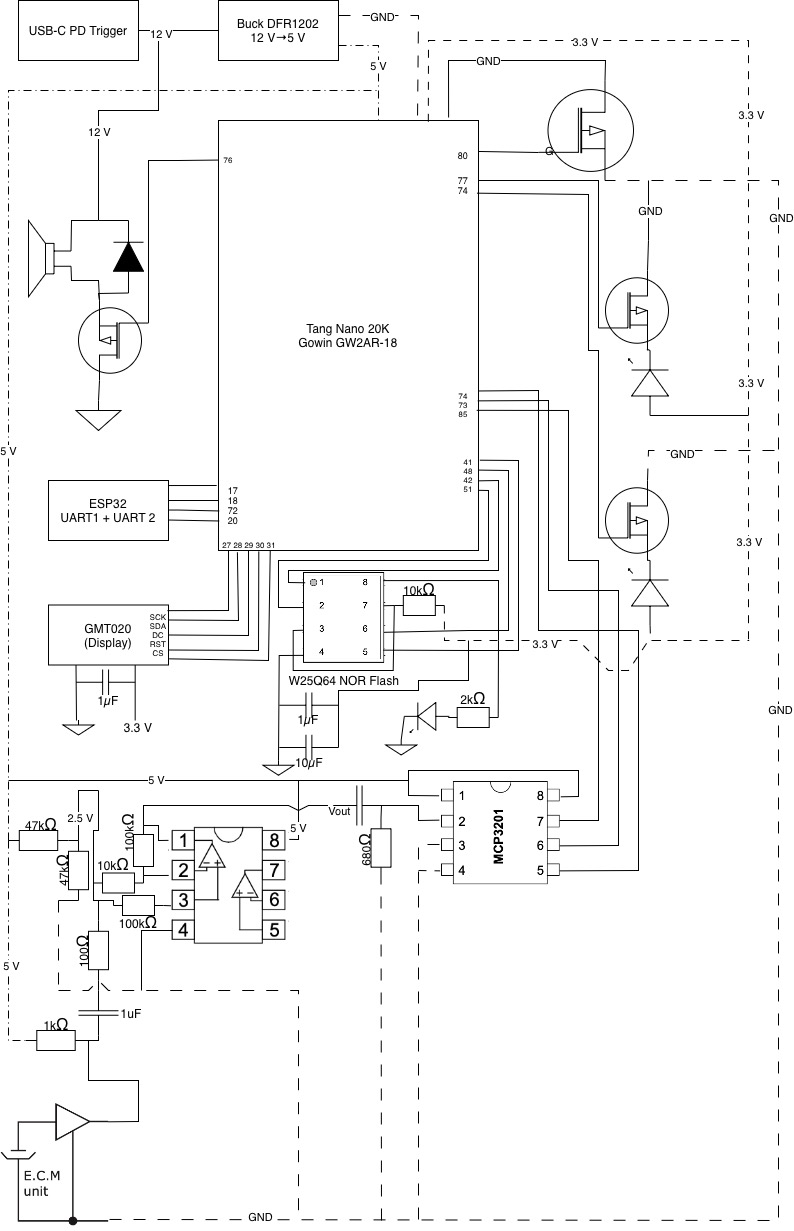
\includegraphics[width=\textwidth]{img/full_circuit_efes.jpg}
\caption{Board level schematic.}
\label{fig:board}
\end{figure}

\begin{figure}[H]
\centering
\resizebox{0.96\textwidth}{!}{%
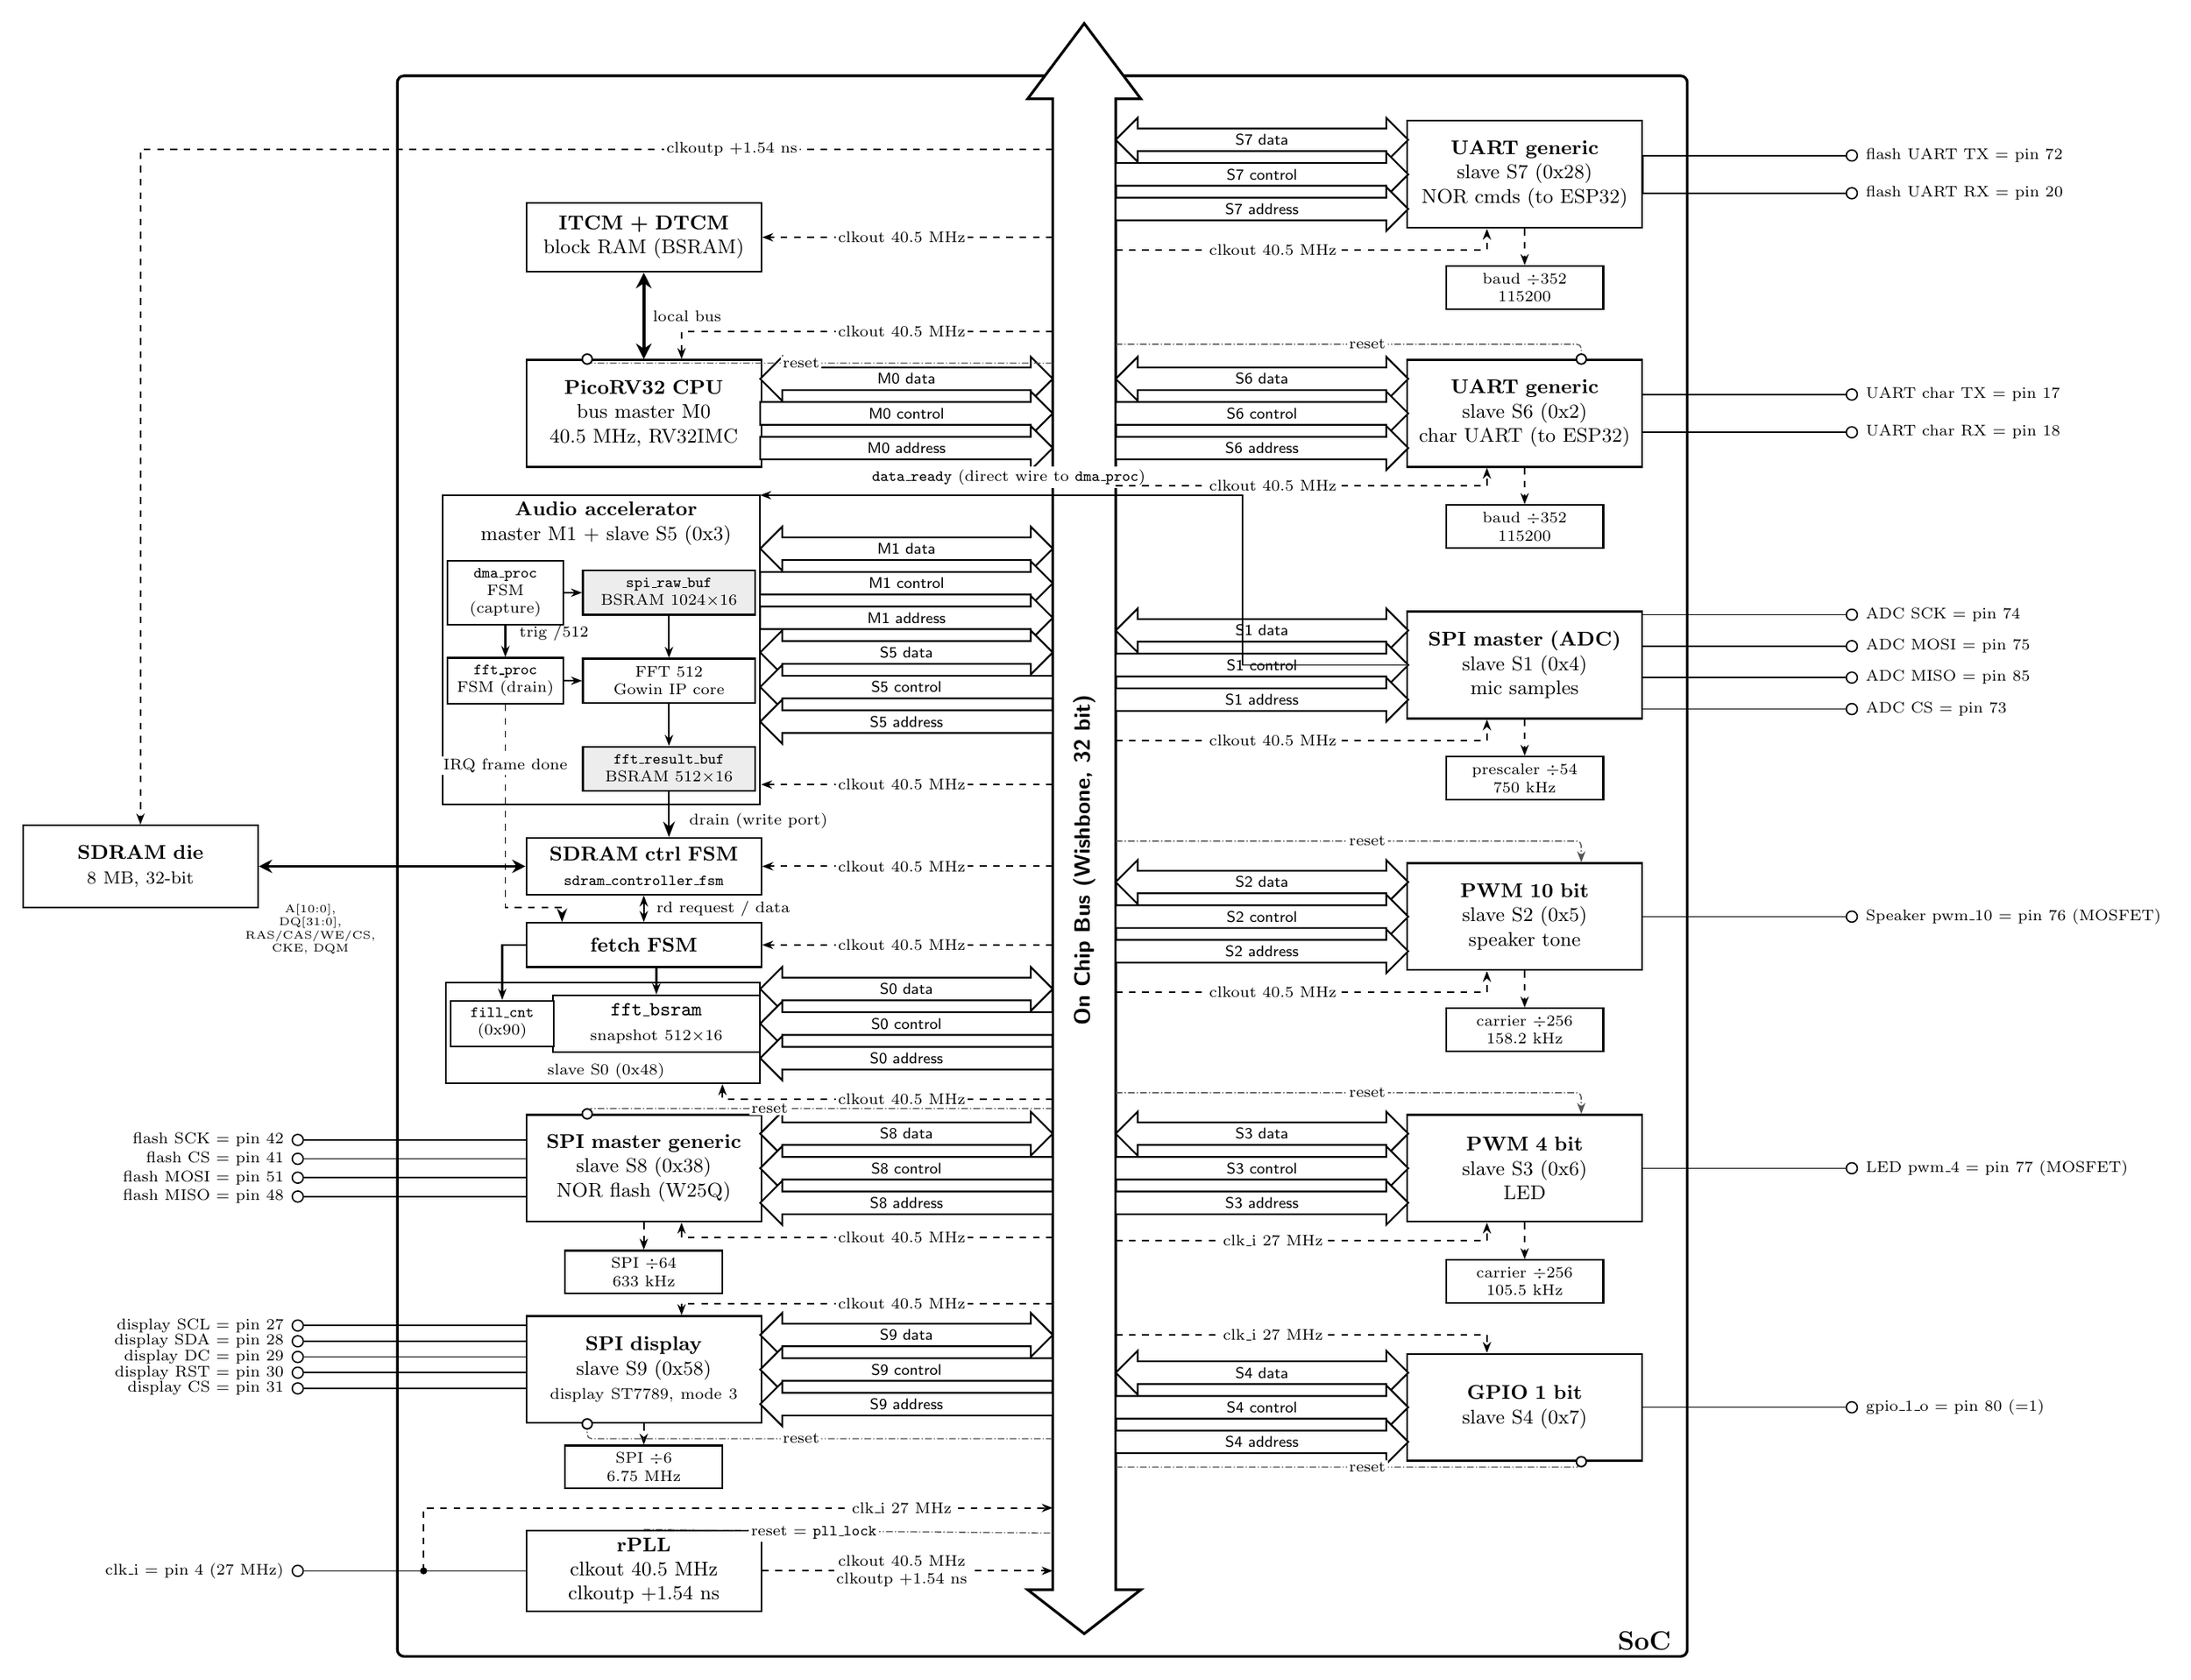
\begin{tikzpicture}[
    every node/.style={font=\small},
    blk/.style={draw, line width=0.8pt, fill=white, minimum width=3.7cm, minimum height=1.7cm, align=center, text width=3.5cm},
    subblk/.style={draw, line width=0.8pt, fill=white, minimum width=1.6cm, minimum height=0.7cm, align=center, font=\scriptsize, text width=1.5cm},
    preblk/.style={draw, line width=0.8pt, fill=white, minimum width=2.5cm, minimum height=0.6cm, align=center, font=\scriptsize},
    pin/.style={circle, draw, fill=white, line width=0.6pt, inner sep=1pt, minimum size=5pt},
    lbl/.style={font=\scriptsize},
    sig/.style={line width=0.6pt},
    clk/.style={-{Stealth[length=5pt]}, line width=0.7pt, dashed},
    rstl/.style={line width=0.48pt, draw=black!68, densely dashdotted, rounded corners=2pt},
    rstar/.style={-{Stealth[length=5pt]}, line width=0.52pt, draw=black!68, densely dashdotted, rounded corners=2pt},
    rstdot/.style={circle, draw, line width=0.7pt, fill=white, inner sep=0pt, minimum size=4.5pt}
]
\newcommand{\fatR}[4]{
    \draw[fill=white, line width=0.8pt]
        (#1, #3+0.18) -- (#2-0.35, #3+0.18) -- (#2-0.35, #3+0.35) --
        (#2, #3) --
        (#2-0.35, #3-0.35) -- (#2-0.35, #3-0.18) -- (#1, #3-0.18) -- cycle;
    \node[font=\scriptsize\sffamily] at ($(#1, #3)!0.5!(#2, #3)$) {#4};
}
\newcommand{\fatL}[4]{
    \draw[fill=white, line width=0.8pt]
        (#2, #3+0.18) -- (#1+0.35, #3+0.18) -- (#1+0.35, #3+0.35) --
        (#1, #3) --
        (#1+0.35, #3-0.35) -- (#1+0.35, #3-0.18) -- (#2, #3-0.18) -- cycle;
    \node[font=\scriptsize\sffamily] at ($(#1, #3)!0.5!(#2, #3)$) {#4};
}
\newcommand{\fatBidir}[4]{
    \draw[fill=white, line width=0.8pt]
        (#1+0.35, #3+0.18) -- (#2-0.35, #3+0.18) -- (#2-0.35, #3+0.35) --
        (#2, #3) --
        (#2-0.35, #3-0.35) -- (#2-0.35, #3-0.18) -- (#1+0.35, #3-0.18) --
        (#1+0.35, #3-0.35) -- (#1, #3) -- (#1+0.35, #3+0.35) -- cycle;
    \node[font=\scriptsize\sffamily] at ($(#1, #3)!0.5!(#2, #3)$) {#4};
}
\def\BusL{-0.5} \def\BusR{0.5}
\def\Ledge{-5.15} \def\Redge{5.15}

% central bus
\draw[fill=white, line width=1.2pt]
    (-0.5, -9.5) -- (-0.5, 14.2) -- (-0.9, 14.2) -- (0, 15.4) --
    (0.9, 14.2) -- (0.5, 14.2) -- (0.5, -9.5) -- (0.9, -9.5) --
    (0, -10.2) -- (-0.9, -9.5) -- cycle;
\node[rotate=90, font=\bfseries\sffamily] at (0, 2.1) {On Chip Bus (Wishbone, 32 bit)};

% left column
\node[blk] (L1) at (-7.0, 9.2) {\textbf{PicoRV32 CPU}\\bus master M0\\40.5 MHz, RV32IMC};
\fatBidir{\Ledge}{\BusL}{9.2+0.55}{M0 data}
\fatR{\Ledge}{\BusL}{9.2}{M0 control}
\fatR{\Ledge}{\BusL}{9.2-0.55}{M0 address}

\fatBidir{\Ledge}{\BusL}{7.05}{M1 data}
\fatR{\Ledge}{\BusL}{6.5}{M1 control}
\fatR{\Ledge}{\BusL}{5.95}{M1 address}
\fatBidir{\Ledge}{\BusL}{5.4}{S5 data}
\fatL{\Ledge}{\BusL}{4.85}{S5 control}
\fatL{\Ledge}{\BusL}{4.3}{S5 address}

\node[blk, minimum height=0.9cm] (L3) at (-7.0, 2.0) {\textbf{SDRAM ctrl FSM}\\\scriptsize \texttt{sdram\_controller\_fsm}};
\node[blk, minimum height=0.7cm] (fetchN) at (-7.0, 0.75) {\textbf{fetch FSM}};
\node[blk, minimum width=3.2cm, text width=3.05cm, minimum height=0.9cm] (bsramN) at (-6.8, -0.5) {\texttt{fft\_bsram}\\\scriptsize snapshot $512{\times}16$};
\node[subblk, minimum width=1.5cm, text width=1.4cm, minimum height=0.7cm] (fillcnt) at (-9.25, -0.5) {\texttt{fill\_cnt}\\(0x90)};
\node[lbl] (s0lbl) at (-7.6, -1.25) {slave S0 (0x48)};
\node[draw, line width=0.8pt, minimum width=5.0cm, minimum height=1.6cm, inner sep=0pt] (s0box) at (-7.65, -0.65) {};
\draw[{Stealth[length=5pt]}-{Stealth[length=5pt]}, line width=0.8pt] (L3.south) -- (fetchN.north)
  node[midway, anchor=west, lbl, xshift=2pt]{rd request / data};
\draw[-{Stealth[length=5pt]}, line width=0.8pt] (fetchN.south -| bsramN.north) -- (bsramN.north);
\draw[-{Stealth[length=5pt]}, line width=0.8pt] (fetchN.west) -| (fillcnt.north);
\fatBidir{\Ledge}{\BusL}{-0.5+0.55}{S0 data}
\fatL{\Ledge}{\BusL}{-0.5}{S0 control}
\fatL{\Ledge}{\BusL}{-0.5-0.55}{S0 address}

\node[blk] (L4) at (-7.0, -2.8) {\textbf{SPI master generic}\\slave S8 (0x38)\\NOR flash (W25Q)};
\node[preblk] (preL4) at (-7.0, -4.45) {SPI $\div$64\\633 kHz};
\draw[clk] (L4.south) -- (preL4.north);
\fatBidir{\Ledge}{\BusL}{-2.8+0.55}{S8 data}
\fatL{\Ledge}{\BusL}{-2.8}{S8 control}
\fatL{\Ledge}{\BusL}{-2.8-0.55}{S8 address}

\node[blk] (disp) at (-7.0, -6.0) {\textbf{SPI display}\\slave S9 (0x58)\\\scriptsize display ST7789, mode 3};
\node[preblk] (preDisp) at (-7.0, -7.55) {SPI $\div$6\\6.75 MHz};
\draw[clk] (disp.south) -- (preDisp.north);
\fatBidir{\Ledge}{\BusL}{-6.0+0.55}{S9 data}
\fatL{\Ledge}{\BusL}{-6.0}{S9 control}
\fatL{\Ledge}{\BusL}{-6.0-0.55}{S9 address}

% right column
\node[blk] (R0) at (7.0, 13.0) {\textbf{UART generic}\\slave S7 (0x28)\\NOR cmds (to ESP32)};
\node[preblk] (preR0) at (7.0, 11.2) {baud $\div$352\\115200};
\draw[clk] (R0.south) -- (preR0.north);
\fatBidir{\BusR}{\Redge}{13.0+0.55}{S7 data}
\fatR{\BusR}{\Redge}{13.0}{S7 control}
\fatR{\BusR}{\Redge}{13.0-0.55}{S7 address}

\node[blk] (R1) at (7.0, 9.2) {\textbf{UART generic}\\slave S6 (0x2)\\char UART (to ESP32)};
\node[preblk] (preR1) at (7.0, 7.4) {baud $\div$352\\115200};
\draw[clk] (R1.south) -- (preR1.north);
\fatBidir{\BusR}{\Redge}{9.2+0.55}{S6 data}
\fatR{\BusR}{\Redge}{9.2}{S6 control}
\fatR{\BusR}{\Redge}{9.2-0.55}{S6 address}

\node[blk] (R2) at (7.0, 5.2) {\textbf{SPI master (ADC)}\\slave S1 (0x4)\\mic samples};
\node[preblk] (preR2) at (7.0, 3.4) {prescaler $\div$54\\750 kHz};
\draw[clk] (R2.south) -- (preR2.north);
\fatBidir{\BusR}{\Redge}{5.2+0.55}{S1 data}
\fatR{\BusR}{\Redge}{5.2}{S1 control}
\fatR{\BusR}{\Redge}{5.2-0.55}{S1 address}

\node[blk] (R3) at (7.0, 1.2) {\textbf{PWM 10 bit}\\slave S2 (0x5)\\speaker tone};
\node[preblk] (preR3) at (7.0, -0.6) {carrier $\div$256\\158.2 kHz};
\draw[clk] (R3.south) -- (preR3.north);
\fatBidir{\BusR}{\Redge}{1.2+0.55}{S2 data}
\fatR{\BusR}{\Redge}{1.2}{S2 control}
\fatR{\BusR}{\Redge}{1.2-0.55}{S2 address}

\node[blk] (R4) at (7.0, -2.8) {\textbf{PWM 4 bit}\\slave S3 (0x6)\\LED};
\node[preblk] (preR4) at (7.0, -4.6) {carrier $\div$256\\105.5 kHz};
\draw[clk] (R4.south) -- (preR4.north);
\fatBidir{\BusR}{\Redge}{-2.8+0.55}{S3 data}
\fatR{\BusR}{\Redge}{-2.8}{S3 control}
\fatR{\BusR}{\Redge}{-2.8-0.55}{S3 address}

\node[blk] (R5) at (7.0, -6.6) {\textbf{GPIO 1 bit}\\slave S4 (0x7)};
\fatBidir{\BusR}{\Redge}{-6.6+0.55}{S4 data}
\fatR{\BusR}{\Redge}{-6.6}{S4 control}
\fatR{\BusR}{\Redge}{-6.6-0.55}{S4 address}

% memories, pll
\node[blk, minimum width=3.0cm, minimum height=1.1cm] (mem) at (-7.0,12.0) {\textbf{ITCM + DTCM}\\block RAM (BSRAM)};
\draw[{Stealth[length=7pt,width=7pt]}-{Stealth[length=7pt,width=7pt]}, line width=1.5pt] (mem.south) -- (L1.north) node[midway, right, lbl]{local bus};

\node[blk, minimum width=3.2cm, minimum height=1.2cm] (pll) at (-7.0,-9.2) {\textbf{rPLL}\\clkout 40.5 MHz\\clkoutp $+1.54$ ns};

% audio accelerator internals
\node[align=center, font=\small] (acctitle) at (-7.6, 7.45) {\textbf{Audio accelerator}\\master M1 + slave S5 (0x3)};
\node[subblk, minimum width=1.7cm, text width=1.6cm] (dmaP)    at (-9.2, 6.35) {\texttt{dma\_proc}\\FSM (capture)};
\node[subblk, fill=black!7, minimum width=2.6cm, text width=2.5cm] (rawB) at (-6.6, 6.35) {\texttt{spi\_raw\_buf}\\BSRAM $1024{\times}16$};
\node[subblk, minimum width=1.7cm, text width=1.6cm] (fftproc) at (-9.2, 4.95) {\texttt{fft\_proc}\\FSM (drain)};
\node[subblk, minimum width=2.6cm, text width=2.5cm] (fftcore) at (-6.6, 4.95) {FFT 512\\Gowin IP core};
\node[subblk, fill=black!7, minimum width=2.6cm, text width=2.5cm] (resbuf) at (-6.6, 3.55) {\texttt{fft\_result\_buf}\\BSRAM $512{\times}16$};
\draw[-{Stealth[length=5pt]}, line width=0.8pt] (dmaP.east) -- (rawB.west);
\draw[-{Stealth[length=5pt]}, line width=0.8pt] (dmaP.south) -- (fftproc.north);
\node[lbl, anchor=west] at (-9.1, 5.7) {trig $/512$};
\draw[-{Stealth[length=5pt]}, line width=0.8pt] (rawB.south) -- (fftcore.north);
\draw[-{Stealth[length=5pt]}, line width=0.8pt] (fftproc.east) -- (fftcore.west);
\draw[-{Stealth[length=5pt]}, line width=0.8pt] (fftcore.south) -- (resbuf.north);
\node[draw, line width=0.8pt, minimum width=5.05cm, minimum height=4.92cm, inner sep=0pt] (L2) at (-7.675, 5.44) {};
% data_ready: direct wire from the ADC SPI (S1) up and over to the top of the accelerator
\draw[-{Stealth[length=5pt]}, line width=0.7pt]
  (R2.west) -- ($(R2.west)+(-2.6,0)$) -- ($(R2.west)+(-2.6,2.7)$) -- (-5.15,7.9);
\node[font=\scriptsize, fill=white, inner sep=1.5pt, anchor=south] at (-1.2,8.0) {\texttt{data\_ready} (direct wire to \texttt{dma\_proc})};

\draw[-{Stealth}, line width=0.9pt] (resbuf.south) -- (L3.north -| resbuf.south);
\node[lbl, anchor=west] at (-6.4, 2.72) {drain (write port)};
\draw[-{Stealth}, line width=0.7pt, dashed] (fftproc.south) -- (-9.2,1.35) -- (-8.3,1.35) -- (fetchN.north -| -8.3,0);
\node[lbl, fill=white, inner sep=1pt] at (-9.2,3.6) {IRQ frame done};

% sdram die
\node[blk, minimum width=2.6cm, minimum height=1.3cm] (die) at (-15.0,2.0) {\textbf{SDRAM die}\\ \footnotesize 8 MB, 32-bit};
\draw[{Stealth[length=6pt,width=6pt]}-{Stealth[length=6pt,width=6pt]}, line width=1.2pt] (die.east) -- (L3.west);
\node[lbl, font=\tiny, align=center] at (-12.3,1.0) {A[10:0],\\DQ[31:0],\\RAS/CAS/WE/CS,\\CKE, DQM};

% external pins
\foreach \i/\y/\nm in {1/-2.35/{flash SCK = pin 42}, 2/-2.65/{flash CS = pin 41}, 3/-2.95/{flash MOSI = pin 51}, 4/-3.25/{flash MISO = pin 48}}{
  \node[pin] (fp\i) at (-12.5,\y){}; \node[lbl,anchor=east] at (fp\i.west){\nm};
  \draw[sig] (fp\i) -- (fp\i -| L4.west);
}
\foreach \i/\y/\nm in {1/-5.3/{display SCL = pin 27}, 2/-5.55/{display SDA = pin 28}, 3/-5.8/{display DC = pin 29}, 4/-6.05/{display RST = pin 30}, 5/-6.3/{display CS = pin 31}}{
  \node[pin] (dp\i) at (-12.5,\y){}; \node[lbl,anchor=east] at (dp\i.west){\nm};
  \draw[sig] (dp\i) -- (dp\i -| disp.west);
}
\node[pin] (xt) at (-12.5,-9.2){}; \node[lbl,anchor=east] at (xt.west){clk\_i = pin 4 (27 MHz)}; \draw[sig](xt)--(pll.west);

\foreach \i/\y/\nm in {1/9.5/{UART char TX = pin 17}, 2/8.9/{UART char RX = pin 18}}{
  \node[pin] (up\i) at (12.2,\y){}; \node[lbl,anchor=west] at (up\i.east){\nm};
  \draw[sig] (up\i -| R1.east) -- (up\i);
}
\node[pin] (fux1) at (12.2,13.3){}; \node[lbl,anchor=west] at (fux1.east){flash UART TX = pin 72};
\node[pin] (fux2) at (12.2,12.7){}; \node[lbl,anchor=west] at (fux2.east){flash UART RX = pin 20};
\draw[sig] (R0.east) |- (fux1);
\draw[sig] (R0.east) |- (fux2);
\foreach \i/\y/\nm in {1/6.0/{ADC SCK = pin 74}, 2/5.5/{ADC MOSI = pin 75}, 3/5.0/{ADC MISO = pin 85}, 4/4.5/{ADC CS = pin 73}}{
  \node[pin] (ap\i) at (12.2,\y){}; \node[lbl,anchor=west] at (ap\i.east){\nm};
  \draw[sig] (ap\i -| R2.east) -- (ap\i);
}
\node[pin] (spk) at (12.2,1.2){}; \node[lbl,anchor=west] at (spk.east){Speaker pwm\_10 = pin 76 (MOSFET)}; \draw[sig](R3.east)--(spk);
\node[pin] (led) at (12.2,-2.8){}; \node[lbl,anchor=west] at (led.east){LED pwm\_4 = pin 77 (MOSFET)}; \draw[sig](R4.east)--(led);
\node[pin] (gp)  at (12.2,-6.6){}; \node[lbl,anchor=west] at (gp.east){gpio\_1\_o = pin 80 (=1)}; \draw[sig](R5.east)--(gp);

% clock tree
\draw[clk] (pll.east) -- (\BusL,-9.2);
\node[lbl, fill=white, inner sep=1pt, align=center] at (-2.9,-9.2) {clkout 40.5 MHz\\clkoutp $+1.54$ ns};
\fill (-10.5,-9.2) circle (1.6pt);
\draw[clk] (-10.5,-9.2) -- (-10.5,-8.2) -- (\BusL,-8.2);
\node[lbl, fill=white, inner sep=1pt] at (-2.9,-8.2) {clk\_i 27 MHz};
\draw[clk] (\BusL,12.0) -- (mem.east);
\node[lbl, fill=white, inner sep=1pt] at (-2.9,12.0) {clkout 40.5 MHz};
\draw[clk] (\BusL,10.5) -| ([xshift=6mm]L1.north);
\node[lbl, fill=white, inner sep=1pt] at (-2.9,10.5) {clkout 40.5 MHz};
\draw[clk] (\BusL,3.3) -- (L2.east |- 0,3.3);
\node[lbl, fill=white, inner sep=1pt] at (-2.9,3.3) {clkout 40.5 MHz};
\draw[clk] (\BusL,2.0) -- (L3.east);
\node[lbl, fill=white, inner sep=1pt] at (-2.9,2.0) {clkout 40.5 MHz};
\draw[clk] (\BusL,0.75) -- (fetchN.east);
\node[lbl, fill=white, inner sep=1pt] at (-2.9,0.75) {clkout 40.5 MHz};
\draw[clk] (\BusL,-1.7) -| ([xshift=19mm]s0box.south);
\node[lbl, fill=white, inner sep=1pt] at (-2.9,-1.7) {clkout 40.5 MHz};
\draw[clk] (\BusL,-3.9) -| ([xshift=6mm]L4.south);
\node[lbl, fill=white, inner sep=1pt] at (-2.9,-3.9) {clkout 40.5 MHz};
\draw[clk] (\BusL,-4.95) -| ([xshift=6mm]disp.north);
\node[lbl, fill=white, inner sep=1pt] at (-2.9,-4.95) {clkout 40.5 MHz};
\draw[clk] (\BusL,13.4) -| (die.north);
\node[lbl, fill=white, inner sep=1pt] at (-5.6,13.4) {clkoutp $+1.54$ ns};
\draw[clk] (\BusR,11.8) -| ([xshift=-6mm]R0.south);
\node[lbl, fill=white, inner sep=1pt] at (3.0,11.8) {clkout 40.5 MHz};
\draw[clk] (\BusR,8.05) -| ([xshift=-6mm]R1.south);
\node[lbl, fill=white, inner sep=1pt] at (3.0,8.05) {clkout 40.5 MHz};
\draw[clk] (\BusR,4.0) -| ([xshift=-6mm]R2.south);
\node[lbl, fill=white, inner sep=1pt] at (3.0,4.0) {clkout 40.5 MHz};
\draw[clk] (\BusR,0.0) -| ([xshift=-6mm]R3.south);
\node[lbl, fill=white, inner sep=1pt] at (3.0,0.0) {clkout 40.5 MHz};
\draw[clk] (\BusR,-3.95) -| ([xshift=-6mm]R4.south);
\node[lbl, fill=white, inner sep=1pt] at (3.0,-3.95) {clk\_i 27 MHz};
\draw[clk] (\BusR,-5.45) -| ([xshift=-6mm]R5.north);
\node[lbl, fill=white, inner sep=1pt] at (3.0,-5.45) {clk\_i 27 MHz};

% reset tree
\draw[rstl] (pll.north) -- (\BusL,-8.6);
\node[lbl, fill=white, inner sep=1pt] at (-4.3,-8.6) {reset $=$ \texttt{pll\_lock}};
\draw[rstl] (\BusL,10.0) -| ([xshift=-9mm]L1.north);
\node[rstdot] at ([xshift=-9mm]L1.north) {};
\node[lbl, fill=white, inner sep=1pt] at (-4.5,10.0) {reset};
\draw[rstl] (\BusL,-1.85) -| ([xshift=-9mm]L4.north);
\node[rstdot] at ([xshift=-9mm]L4.north) {};
\node[lbl, fill=white, inner sep=1pt] at (-5.0,-1.85) {reset};
\draw[rstl] (\BusL,-7.1) -| ([xshift=-9mm]disp.south);
\node[rstdot] at ([xshift=-9mm]disp.south) {};
\node[lbl, fill=white, inner sep=1pt] at (-4.5,-7.1) {reset};
\draw[rstl] (\BusR,10.3) -| ([xshift=9mm]R1.north);
\node[rstdot] at ([xshift=9mm]R1.north) {};
\node[lbl, fill=white, inner sep=1pt] at (4.5,10.3) {reset};
\draw[rstl] (\BusR,-7.55) -| ([xshift=9mm]R5.south);
\node[rstdot] at ([xshift=9mm]R5.south) {};
\node[lbl, fill=white, inner sep=1pt] at (4.5,-7.55) {reset};
\draw[rstar] (\BusR,2.4) -| ([xshift=9mm]R3.north);
\node[lbl, fill=white, inner sep=1pt] at (4.5,2.4) {reset};
\draw[rstar] (\BusR,-1.6) -| ([xshift=9mm]R4.north);
\node[lbl, fill=white, inner sep=1pt] at (4.5,-1.6) {reset};

% soc bounding box
\begin{scope}[on background layer]
\node[draw, line width=1.2pt, fit=(mem)(L2)(L4)(preL4)(disp)(pll)(R0)(preR0)(R1)(preR1)(R5)(preR4), inner sep=20pt, rounded corners=3pt] (socbox){};
\end{scope}
\node[anchor=south east, font=\bfseries\large] at (socbox.south east) {SoC\ \ };

\end{tikzpicture}%
}
\caption{SoC top level block diagram.}
\label{fig:soc}
\end{figure}

% =====================================================================
\section{Power management}
\label{sec:power}
% =====================================================================

The board runs on three rails (Figure~\ref{fig:power}). A USB-C PD trigger gives 12\,V. The
12\,V feeds two things: the speaker stage directly, and the input of a DFR1202 buck. The
buck makes 5\,V, and the 5\,V feeds the board \texttt{VIN} and the analog front end. An on
board regulator then makes 3.3\,V from the 5\,V, and the 3.3\,V feeds the digital
peripherals, the NOR flash, the display and the LEDs, through the GPIO switch described
below.

Every switched load is driven low side: the control pin drives the gate of an N channel
IRLZ44N MOSFET, the load sits between its supply and the drain, and when the gate goes high
the MOSFET pulls the drain to ground so current flows. The gate is referenced to ground, so
the 3.3\,V logic level turns it on with no gate driver, and the speaker has a flyback diode
for its inductance. The speaker and the LEDs are switched this way by their PWM pins.

The 3.3\,V to the peripherals passes through one more IRLZ44N, gated by \texttt{gpio\_1}
(pin 80). This is a soft power switch: the CPU can cut power to the NOR flash, the display
and the LEDs by driving the pin low, so the pin must stay at \texttt{'1'} in normal use.

\begin{figure}[H]
\centering
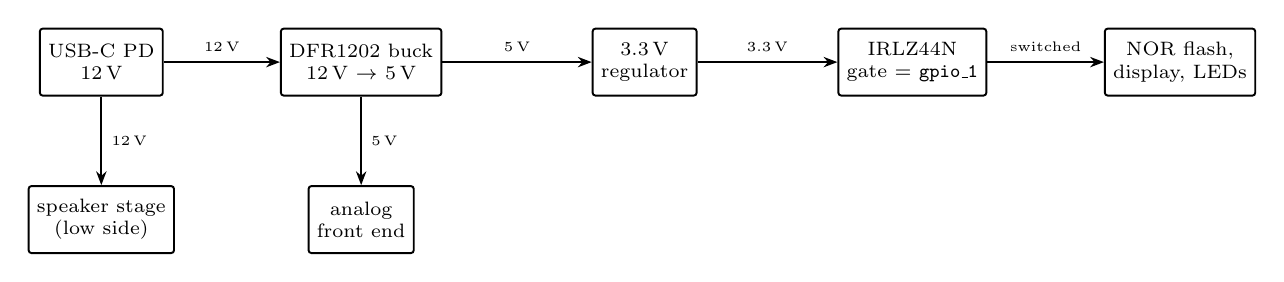
\begin{tikzpicture}[
  every node/.style={font=\scriptsize},
  b/.style={draw, line width=0.7pt, fill=white, align=center, rounded corners=1pt, inner sep=3pt, minimum height=0.85cm},
  a/.style={-{Stealth[length=5pt]}, line width=0.7pt}]
\node[b] (usb) at (0,0)    {USB-C PD\\ 12\,V};
\node[b] (buck) at (3.3,0) {DFR1202 buck\\ 12\,V $\to$ 5\,V};
\node[b] (reg) at (6.9,0)  {3.3\,V\\ regulator};
\node[b] (sw) at (10.3,0)  {IRLZ44N\\ gate $=$ \texttt{gpio\_1}};
\node[b] (per) at (13.7,0) {NOR flash,\\ display, LEDs};
\node[b] (spk) at (0,-2.0)   {speaker stage\\ (low side)};
\node[b] (afe) at (3.3,-2.0) {analog\\ front end};
\draw[a] (usb) -- node[above,font=\tiny]{12\,V}(buck);
\draw[a] (buck) -- node[above,font=\tiny]{5\,V}(reg);
\draw[a] (reg) -- node[above,font=\tiny]{3.3\,V}(sw);
\draw[a] (sw) -- node[above,font=\tiny]{switched}(per);
\draw[a] (usb.south) -- node[right,font=\tiny]{12\,V}(spk.north);
\draw[a] (buck.south) -- node[right,font=\tiny]{5\,V}(afe.north);
\end{tikzpicture}
\caption{Power tree.}
\label{fig:power}
\end{figure}

% =====================================================================
\section{The SDRAM controller}
\label{sec:sdram}
% =====================================================================

The GW2AR-18 package contains an 8\,MB SDRAM die, organized into 4 banks, and each bank
is a grid of 2048 rows $\times$ 256 columns, where every cell holds one 32 bit word
(so a row is 256 words $=$ 1\,KB, and $4\times2048\times256\times4 = 8$\,MB).
Based on the datasheet and the manufacturer's timing diagrams, 
the memory operates using burst transfers. A single read (\texttt{rd\_n})
 or write (\texttt{wr\_n}) command, accompanied by a 21 bit address specifying the bank,
 row, and column, triggers a data burst of \texttt{data\_len}$+1$ words.
 In my design, \texttt{data\_len} is set to 26, resulting in a 27 word burst.
The operation is managed by a few key control signals: \texttt{busy\_n} 
indicates when the controller is ready to accept a new command request;
 \texttt{rd\_valid} confirms that the current read word is valid data; 
 and \texttt{init\_done} signals that the power up initialization sequence is complete.

Figure~\ref{fig:sdram-struct} shows how one bank is addressed, and its two
access delays.

\begin{figure}[H]
\centering
\resizebox{!}{5cm}{%
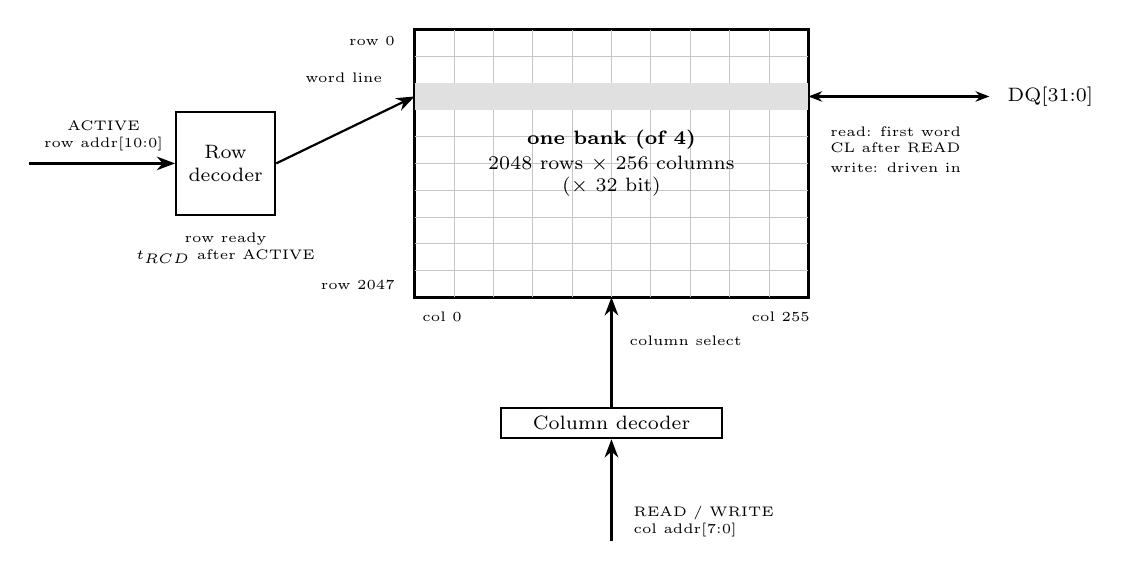
\begin{tikzpicture}[
  every node/.style={font=\scriptsize},
  blk/.style={draw, line width=0.7pt, fill=white, align=center, inner sep=3pt},
  >={Stealth}, line width=0.8pt,
  gl/.style={gray!45, line width=0.3pt}
]
\def\W{5.0}\def\H{3.4}
% the array
\draw[line width=0.9pt] (0,0) rectangle (\W,\H);
\foreach \y in {0.34,0.68,...,3.06}{ \draw[gl] (0,\y) -- (\W,\y); }
\foreach \x in {0.5,1.0,...,4.5}{ \draw[gl] (\x,0) -- (\x,\H); }
% open row highlighted
\fill[black!12] (0,2.38) rectangle (\W,2.72);
% dimension labels
\node[anchor=east, font=\tiny] at (-0.12,\H-0.15) {row 0};
\node[anchor=east, font=\tiny] at (-0.12,0.16) {row 2047};
\node[anchor=north, font=\tiny] at (0.35,-0.06) {col 0};
\node[anchor=north, font=\tiny] at (\W-0.35,-0.06) {col 255};
\node[align=center] at ({\W/2},{\H/2}) {\textbf{one bank (of 4)}\\[1pt] 2048 rows $\times$ 256 columns\\ ($\times$ 32 bit)};
% row decoder + ACTIVE
\node[blk, minimum height=1.3cm, text width=1.05cm] (rowd) at (-2.4,{\H/2}) {Row\\ decoder};
\draw[->] (rowd.east) -- (0,2.55);
\node[font=\tiny, anchor=south] at (-0.9,2.6) {word line};
\draw[->] (-4.9,{\H/2}) -- (rowd.west);
\node[font=\tiny, anchor=south, align=center] at (-3.95,{\H/2+0.03}) {ACTIVE\\ row addr[10:0]};
\node[font=\tiny, align=center, anchor=north] at (-2.4,{\H/2-0.75}) {row ready\\ $t_{RCD}$ after ACTIVE};
% column decoder + READ/WRITE
\node[blk, minimum width=2.8cm] (cold) at ({\W/2},-1.6) {Column decoder};
\draw[->] (cold.north) -- ({\W/2},0);
\node[font=\tiny, anchor=west] at ({\W/2+0.1},-0.55) {column select};
\draw[->] ({\W/2},-3.1) -- (cold.south);
\node[font=\tiny, anchor=west, align=left] at ({\W/2+0.15},-2.85) {READ / WRITE\\ col addr[7:0]};
% data out / in
\draw[{Stealth[length=5pt]}-{Stealth[length=5pt]}, line width=1.2pt] (\W,2.55) -- ++(2.3,0);
\node[anchor=west] at ({\W+2.4},2.55) {DQ[31:0]};
\node[font=\tiny, align=left, anchor=north west] at ({\W+0.15},2.3)
  {read: first word\\ CL after READ\\[1pt] write: driven in};
\end{tikzpicture}%
}
\caption{One SDRAM bank: 2048 rows by 256 columns, and how a row and a column are
selected, with the two access delays.}
\label{fig:sdram-struct}
\end{figure}

\subsection{The FSM}

A combinational process
computes \texttt{next\_state} only, and a synchronous process registers the state,
one shared counter \texttt{tmr} (cleared on every state change), and \emph{all}
outputs a Moore machine with registered outputs, where each JEDEC command is
emitted exactly on the first cycle of its state (detected as
\texttt{next\_state\,$\neq$\,curr\_state}) and NOP fills the rest. The mode register is
programmed for CAS latency 3 (CL is the one timing I set myself; I use 3 because it only
adds two cycles over CL 1 and changes nothing for the project constraints, and this way I am sure there is no
problem on that side), sequential addressing and \emph{full page} burst. This is why the
column address goes out only once, with the READ or WRITE command: from there the die
steps through the columns by itself, one per cycle and in order (sequential), so I never
resend it. The burst length is just how long the FSM stays in the data state, and the
closing PRECHARGE ends it. The FSM also issues an AUTO
REFRESH about every $7.8\,\mu$s: a counter asks for one every 312 cycles, served in
\texttt{S\_IDLE}. Table~\ref{tab:sdram-cmd} lists the commands it issues.

\begin{table}[H]
\centering
\caption{The SDRAM commands the FSM issues, and their code on the four control pins
(active low): the FSM never sends the word, it drives this pattern for one cycle.}
\label{tab:sdram-cmd}
\small
\begin{tabular}{l c l}
\toprule
\textbf{Command} & \textbf{$\overline{\mathrm{CS}}\,\overline{\mathrm{RAS}}\,\overline{\mathrm{CAS}}\,\overline{\mathrm{WE}}$} & \textbf{Role} \\
\midrule
ACTIVE             & \texttt{0 0 1 1} & opens a row, copying it into the sense amplifiers \\
READ               & \texttt{0 1 0 1} & reads a column from the open row \\
WRITE              & \texttt{0 1 0 0} & writes a column into the open row \\
PRECHARGE          & \texttt{0 0 1 0} & closes the open row, writing it back \\
AUTO REFRESH       & \texttt{0 0 0 1} & refreshes the rows so they keep their charge \\
LOAD MODE REGISTER & \texttt{0 0 0 0} & sets CAS latency, burst type and length \\
NOP                & \texttt{0 1 1 1} & does nothing, fills the waits between commands \\
\bottomrule
\end{tabular}
\end{table}

I read the JEDEC instruction set from the SDRAM datasheet
and turned each into the number of 40.5\,MHz clock cycles
the FSM has to hold before it issues the following command (Table~\ref{tab:jedec}).
Those cycle counts are exactly the numbers written in the state graph below.

\begin{table}[H]
\centering
\caption{SDRAM timing values read from the datasheet, each converted to 40.5\,MHz clock cycles.}
\label{tab:jedec}
\small
\begin{tabular}{llcc}
\toprule
\textbf{Parameter} & \textbf{Role} & \textbf{Cycles} & \textbf{Wait} \\
\midrule
power up wait & stable clock before init & 8192 & $202\,\mu$s \\
$t_{RCD}$ & ACTIVE to READ/WRITE & 3 & 74\,ns \\
CL & READ to first valid word & 3 & 74\,ns \\
$t_{RP}$ & PRECHARGE to next command & 2 & 49\,ns \\
$t_{RFC}$ & AUTO REFRESH to next command & 4 & 99\,ns \\
$t_{MRD}$ & LOAD MODE REG to next command & 2 & 49\,ns \\
$t_{WR}$ & last write to PRECHARGE & 2 & 49\,ns \\
refresh & one AUTO REFRESH every & 312 & $7.7\,\mu$s \\
\bottomrule
\end{tabular}
\end{table}

\begin{figure}[H]
\centering
\resizebox{0.99\textwidth}{!}{%
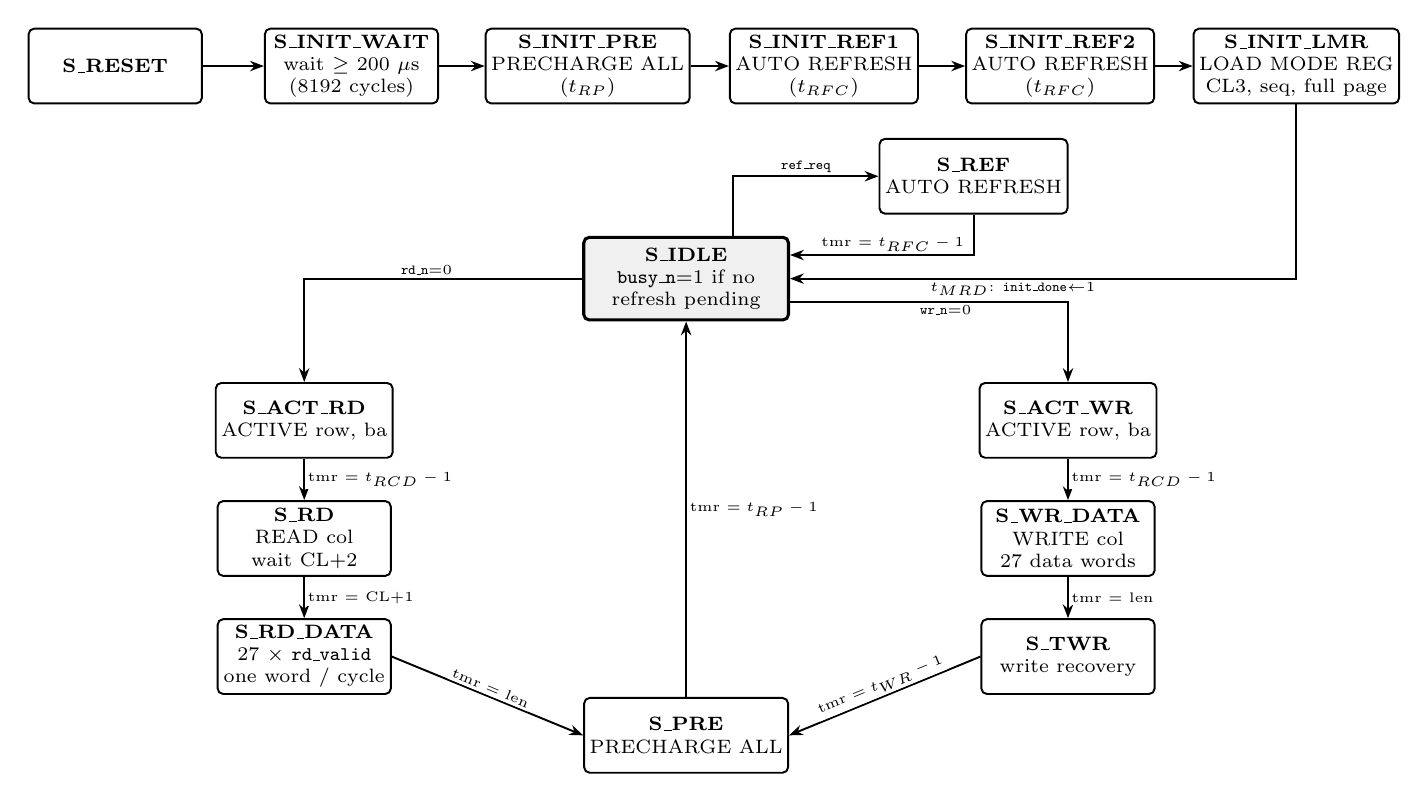
\begin{tikzpicture}[
    every node/.style={font=\footnotesize},
    st/.style={rounded corners=2pt, draw, line width=0.7pt, fill=white, minimum width=2.2cm, minimum height=0.95cm, align=center, inner sep=2pt, font=\scriptsize},
    hub/.style={rounded corners=2pt, draw, line width=1.1pt, fill=black!6, minimum width=2.6cm, minimum height=1.05cm, align=center, inner sep=2pt, font=\scriptsize},
    a/.style={-{Stealth[length=5pt]}, line width=0.7pt},
    al/.style={font=\tiny, fill=white, inner sep=1pt}
]
% init chain
\node[st] (rst)  at (0,3.9)    {\textbf{S\_RESET}};
\node[st] (iw)   at (3.0,3.9)  {\textbf{S\_INIT\_WAIT}\\wait $\geq$ 200 $\mu$s\\(8192 cycles)};
\node[st] (ip)   at (6.0,3.9)  {\textbf{S\_INIT\_PRE}\\PRECHARGE ALL\\($t_{RP}$)};
\node[st] (ir1)  at (9.0,3.9)  {\textbf{S\_INIT\_REF1}\\AUTO REFRESH\\($t_{RFC}$)};
\node[st] (ir2)  at (12.0,3.9) {\textbf{S\_INIT\_REF2}\\AUTO REFRESH\\($t_{RFC}$)};
\node[st] (ilmr) at (15.0,3.9) {\textbf{S\_INIT\_LMR}\\LOAD MODE REG\\CL3, seq, full page};
\draw[a] (rst)--(iw);
\draw[a] (iw)--(ip);
\draw[a] (ip)--(ir1);
\draw[a] (ir1)--(ir2);
\draw[a] (ir2)--(ilmr);
% idle hub
\node[hub] (idle) at (7.25,1.2) {\textbf{S\_IDLE}\\\texttt{busy\_n}=1 if no\\refresh pending};
\draw[a] (ilmr.south) |- node[al, pos=0.78, below]{$t_{MRD}$: \texttt{init\_done}$\leftarrow$1} (idle.east);
% refresh above idle
\node[st] (ref) at (10.9,2.5) {\textbf{S\_REF}\\AUTO REFRESH};
\draw[a] ([xshift=6mm]idle.north) |- node[al, pos=0.75, above]{\texttt{ref\_req}} (ref.west);
\draw[a] (ref.south) |- node[al, pos=0.72, above]{tmr $=t_{RFC}-1$} ([yshift=3mm]idle.east);
% read branch (left)
\node[st] (ard) at (2.4,-0.6)  {\textbf{S\_ACT\_RD}\\ACTIVE row, ba};
\node[st] (rd)  at (2.4,-2.1)  {\textbf{S\_RD}\\READ col\\wait CL$+$2};
\node[st] (rdd) at (2.4,-3.6)  {\textbf{S\_RD\_DATA}\\27 $\times$ \texttt{rd\_valid}\\one word / cycle};
\draw[a] (idle.west) -| node[al, pos=0.28, above]{\texttt{rd\_n}$=$0} (ard.north);
\draw[a] (ard)-- node[al,right]{tmr $=t_{RCD}-1$} (rd);
\draw[a] (rd)-- node[al,right]{tmr $=$ CL$+$1} (rdd);
% write branch (right)
\node[st] (awr) at (12.1,-0.6) {\textbf{S\_ACT\_WR}\\ACTIVE row, ba};
\node[st] (wrd) at (12.1,-2.1) {\textbf{S\_WR\_DATA}\\WRITE col\\27 data words};
\node[st] (twr) at (12.1,-3.6) {\textbf{S\_TWR}\\write recovery};
\draw[a] ([yshift=-3mm]idle.east) -| node[al, pos=0.28, below]{\texttt{wr\_n}$=$0} (awr.north);
\draw[a] (awr)-- node[al,right]{tmr $=t_{RCD}-1$} (wrd);
\draw[a] (wrd)-- node[al,right]{tmr $=$ len} (twr);
% precharge (shared)
\node[st] (pre) at (7.25,-4.6) {\textbf{S\_PRE}\\PRECHARGE ALL};
\draw[a] (rdd.east) -- node[al,above,sloped]{tmr $=$ len} (pre.west);
\draw[a] (twr.west) -- node[al,above,sloped]{tmr $=t_{WR}-1$} (pre.east);
\draw[a] (pre.north) -- node[al,right]{tmr $=t_{RP}-1$} (idle.south);
\end{tikzpicture}%
}
\caption{Complete \texttt{sdram\_controller\_fsm} state graph.}
\label{fig:sdram-fsm}
\end{figure}

\subsection{Bring up sequence}

At power up the die must be initialised in a fixed order before it works. The FSM runs it once and then raises \texttt{init\_done}:
\begin{enumerate}\setlength{\itemsep}{0pt}
\item wait 8192 cycles ($202\,\mu$s) with CKE high;
\item PRECHARGE ALL, to put the four banks in idle;
\item two AUTO REFRESH commands;
\item LOAD MODE REGISTER (CL 3, sequential, full page).
\end{enumerate}
This runs only at boot. After \texttt{init\_done} the controller issues normal commands
plus one AUTO REFRESH every 312 cycles. In the diagram the address line
\texttt{addr[10]} (\texttt{O\_sdram\_addr[10]}) doubles as a control bit: on a PRECHARGE
the chip reads \texttt{addr[10]}$=1$ as ``all four banks'', which is why it is high
during PRECHARGE ALL.

\begin{figure}[H]
\centering
\resizebox{\textwidth}{!}{%
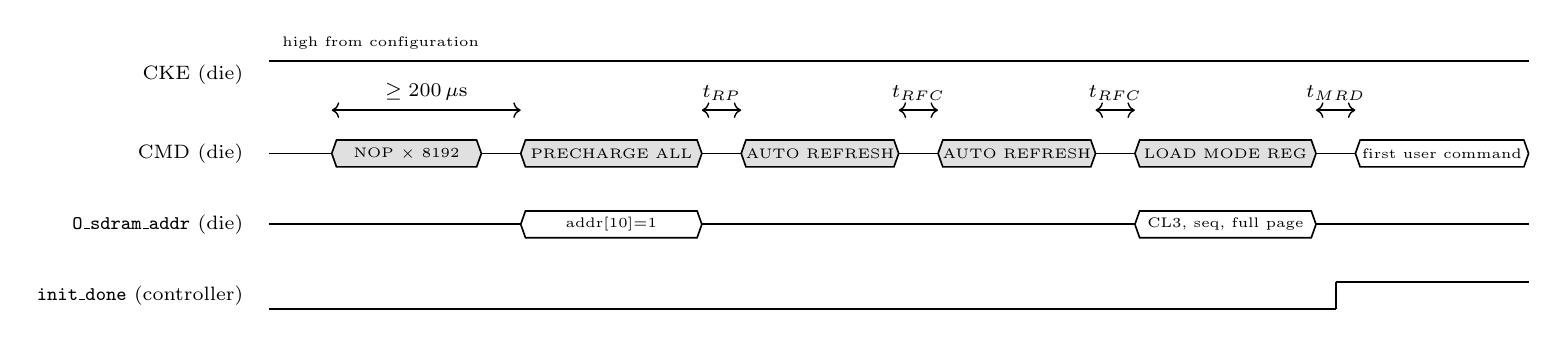
\begin{tikzpicture}[every node/.style={font=\scriptsize}]
\def\Y{0}
% CKE row
\node[anchor=east] at (-0.2,1.0) {CKE (die)};
\draw[line width=0.7pt] (0,1.17) -- (16.0,1.17);
\node[font=\tiny, anchor=south west] at (0.05,1.2) {high from configuration};
% CMD row
\node[anchor=east] at (-0.2,\Y) {CMD (die)};
\widle{0}{0.8}{\Y}
\wbusg{0.8}{2.7}{\Y}{NOP $\times$ 8192}
\widle{2.7}{3.2}{\Y}
\wbusg{3.2}{5.5}{\Y}{PRECHARGE ALL}
\widle{5.5}{6.0}{\Y}
\wbusg{6.0}{8.0}{\Y}{AUTO REFRESH}
\widle{8.0}{8.5}{\Y}
\wbusg{8.5}{10.5}{\Y}{AUTO REFRESH}
\widle{10.5}{11.0}{\Y}
\wbusg{11.0}{13.3}{\Y}{LOAD MODE REG}
\widle{13.3}{13.8}{\Y}
\wbus{13.8}{16.0}{\Y}{first user command}
% A row
\node[anchor=east] at (-0.2,-0.9) {\texttt{O\_sdram\_addr} (die)};
\widle{0}{3.2}{-0.9}
\wbus{3.2}{5.5}{-0.9}{addr[10]$=$1}
\widle{5.5}{11.0}{-0.9}
\wbus{11.0}{13.3}{-0.9}{CL3, seq, full page}
\widle{13.3}{16.0}{-0.9}
% init_done
\node[anchor=east] at (-0.2,-1.8) {\texttt{init\_done} (controller)};
\wlo{0}{13.55}{-1.8}
\wfe{13.55}{-1.8}
\whi{13.55}{16.0}{-1.8}
% annotations
\draw[<->, line width=0.5pt] (0.8,0.55) -- (3.2,0.55);
\node[anchor=south] at (2.0,0.55) {$\geq 200\,\mu$s};
\draw[<->, line width=0.5pt] (5.5,0.55) -- (6.0,0.55);
\node[anchor=south] at (5.75,0.55) {$t_{RP}$};
\draw[<->, line width=0.5pt] (8.0,0.55) -- (8.5,0.55);
\node[anchor=south] at (8.25,0.55) {$t_{RFC}$};
\draw[<->, line width=0.5pt] (10.5,0.55) -- (11.0,0.55);
\node[anchor=south] at (10.75,0.55) {$t_{RFC}$};
\draw[<->, line width=0.5pt] (13.3,0.55) -- (13.8,0.55);
\node[anchor=south] at (13.55,0.55) {$t_{MRD}$};
\end{tikzpicture}%
}
\caption{SDRAM bring up sequence.}
\label{fig:sdram-init}
\end{figure}

\subsection{Read path and clock phase}
\label{sec:sdram-read}

Figure~\ref{fig:sdram-read} shows a read burst cycle by cycle. After a read request
the FSM sends ACTIVE, then READ three cycles later (this wait is $t_{RCD}$), and three
cycles after READ (the CAS latency CL) the die puts the first word on its data pins
(the \texttt{DQ} bus). Both waits, and the others further down, are the JEDEC numbers
listed in Table~\ref{tab:jedec}. The SDRAM has no valid
line of its own, so the controller times the read by counting. The word passes through
two flip flops inside the controller: the first one captures the data pins
coming from the die, the second one holds that word ready. When the word reaches the
second flip flop the FSM raises \texttt{rd\_valid}, which tells that
the word on \texttt{O\_sdrc\_data} is good. So \texttt{rd\_valid} goes high CL$+2$
cycles after READ, one extra cycle per flip flop, and stays up for the 27 words, one
per cycle.

\textbf{Clock phase.} On a read the die does not drive its data pins at once: the data
comes a few nanoseconds after the die's clock edge (the access time $t_{AC}$) and then
travels back over the board to the FPGA, so it arrives late. With the die on the same
clock as the controller I was sampling too early, and on a small fraction of reads a
bit came back wrong (\texttt{0xFFFE} instead of \texttt{0xFFFF}). Feeding the die the $1.54$\,ns shifted
clock (\texttt{clkoutp}) lets me sample in the middle of the data, and the errors
stopped.

\begin{figure}[H]
\centering
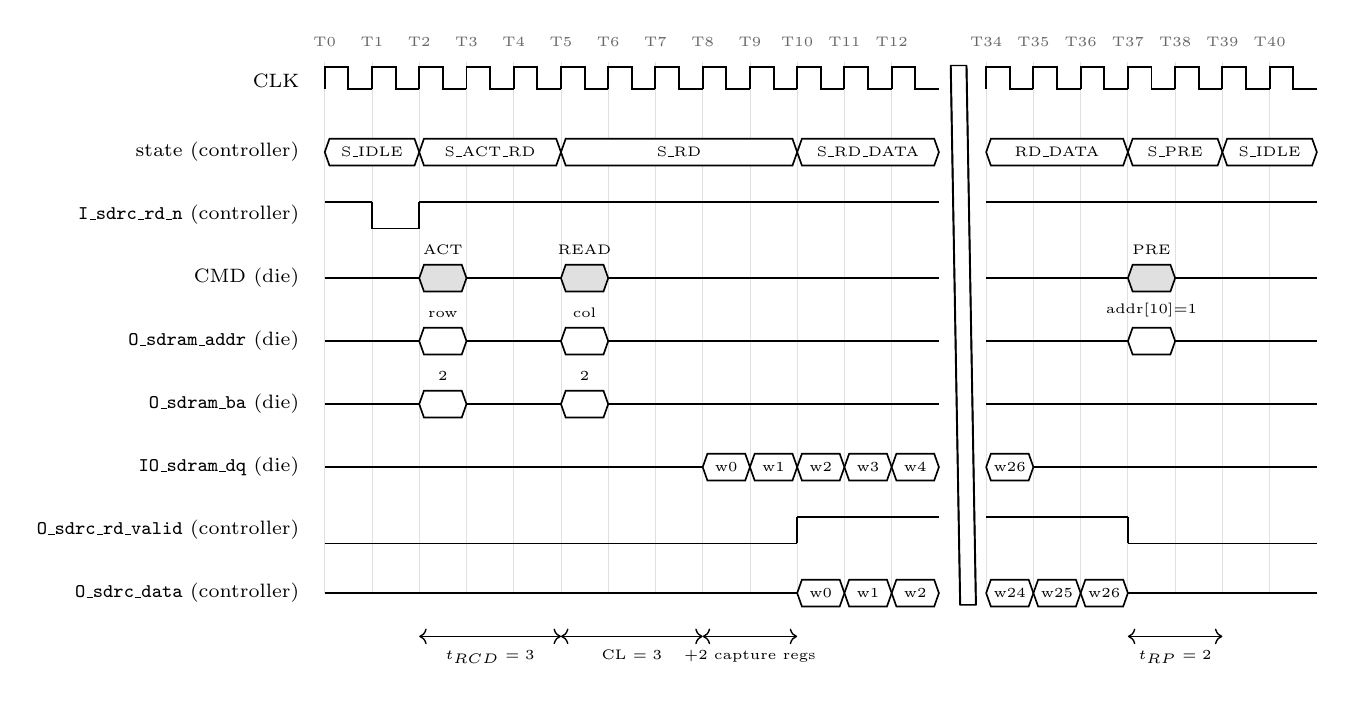
\begin{tikzpicture}[every node/.style={font=\scriptsize}]
\def\NA{13}
\def\XB{8.4}  % start x of part B
\def\NB{7}
% ticks and grid
\wticks{0}{12}{0.42}{0}
\wgrid{0}{12}{0.35}{-6.4}
\wticks{\XB}{6}{0.42}{34}
\wgrid{\XB}{6}{0.35}{-6.4}
% CLK
\wlab{CLK}{0.1}
\wclk{0}{13}{0}
\wclk{\XB}{7}{0}
% state row
\wlab{state (controller)}{-0.8}
\wbus{0}{1.2}{-0.8}{S\_IDLE}
\wbus{1.2}{3.0}{-0.8}{S\_ACT\_RD}
\wbus{3.0}{6.0}{-0.8}{S\_RD}
\wbus{6.0}{7.8}{-0.8}{S\_RD\_DATA}
\wbus{\XB}{10.2}{-0.8}{RD\_DATA}
\wbus{10.2}{11.4}{-0.8}{S\_PRE}
\wbus{11.4}{12.6}{-0.8}{S\_IDLE}
% rd_n
\wlab{\texttt{I\_sdrc\_rd\_n} (controller)}{-1.6}
\whi{0}{0.6}{-1.6}\wfe{0.6}{-1.6}\wlo{0.6}{1.2}{-1.6}\wfe{1.2}{-1.6}\whi{1.2}{7.8}{-1.6}
\whi{\XB}{12.6}{-1.6}
% CMD
\wlab{CMD (die)}{-2.4}
\widle{0}{1.2}{-2.4}
\wcmd{1.2}{1.8}{-2.4}{ACT}
\widle{1.8}{3.0}{-2.4}
\wcmd{3.0}{3.6}{-2.4}{READ}
\widle{3.6}{7.8}{-2.4}
\widle{\XB}{10.2}{-2.4}
\wcmd{10.2}{10.8}{-2.4}{PRE}
\widle{10.8}{12.6}{-2.4}
% A / BA
\wlab{\texttt{O\_sdram\_addr} (die)}{-3.2}
\widle{0}{1.2}{-3.2}
\wval{1.2}{1.8}{-3.2}{row}
\widle{1.8}{3.0}{-3.2}
\wval{3.0}{3.6}{-3.2}{col}
\widle{3.6}{7.8}{-3.2}
\widle{\XB}{10.2}{-3.2}
\wval{10.2}{10.8}{-3.2}{addr[10]$=$1}
\widle{10.8}{12.6}{-3.2}
% BA
\wlab{\texttt{O\_sdram\_ba} (die)}{-4.0}
\widle{0}{1.2}{-4.0}
\wval{1.2}{1.8}{-4.0}{2}
\widle{1.8}{3.0}{-4.0}
\wval{3.0}{3.6}{-4.0}{2}
\widle{3.6}{7.8}{-4.0}
\widle{\XB}{10.2}{-4.0}
\widle{10.2}{12.6}{-4.0}
% DQ from die
\wlab{\texttt{IO\_sdram\_dq} (die)}{-4.8}
\widle{0}{4.8}{-4.8}
\wbus{4.8}{5.4}{-4.8}{w0}
\wbus{5.4}{6.0}{-4.8}{w1}
\wbus{6.0}{6.6}{-4.8}{w2}
\wbus{6.6}{7.2}{-4.8}{w3}
\wbus{7.2}{7.8}{-4.8}{w4}
\wbus{\XB}{9.0}{-4.8}{w26}
\widle{9.0}{12.6}{-4.8}
% rd_valid
\wlab{\texttt{O\_sdrc\_rd\_valid} (controller)}{-5.6}
\wlo{0}{6.0}{-5.6}\wfe{6.0}{-5.6}\whi{6.0}{7.8}{-5.6}
\whi{\XB}{10.2}{-5.6}\wfe{10.2}{-5.6}\wlo{10.2}{12.6}{-5.6}
% data out
\wlab{\texttt{O\_sdrc\_data} (controller)}{-6.4}
\widle{0}{6.0}{-6.4}
\wbus{6.0}{6.6}{-6.4}{w0}
\wbus{6.6}{7.2}{-6.4}{w1}
\wbus{7.2}{7.8}{-6.4}{w2}
\wbus{\XB}{9.0}{-6.4}{w24}
\wbus{9.0}{9.6}{-6.4}{w25}
\wbus{9.6}{10.2}{-6.4}{w26}
\widle{10.2}{12.6}{-6.4}
% cut marks
\wcut{8.05}{0.3}{-6.55}
% brackets
\draw[<->, line width=0.5pt] (1.2,-6.95) -- (3.0,-6.95);
\node[anchor=north, font=\tiny] at (2.1,-7) {$t_{RCD}=3$};
\draw[<->, line width=0.5pt] (3.0,-6.95) -- (4.8,-6.95);
\node[anchor=north, font=\tiny] at (3.9,-7) {CL $=3$};
\draw[<->, line width=0.5pt] (4.8,-6.95) -- (6.0,-6.95);
\node[anchor=north, font=\tiny] at (5.4,-7) {$+2$ capture regs};
\draw[<->, line width=0.5pt] (10.2,-6.95) -- (11.4,-6.95);
\node[anchor=north, font=\tiny] at (10.8,-7) {$t_{RP}=2$};
\end{tikzpicture}
\caption{Read burst, cycle accurate.}
\label{fig:sdram-read}
\end{figure}

\subsection{Write path}
\label{sec:sdram-write}

On a write the FSM sends one word per cycle. The controller has to line the words up so that
word 0 lands on the data pins in the same cycle as the WRITE command, which
goes out three cycles after ACTIVE (the $t_{RCD}$ wait of Table~\ref{tab:jedec}). It does this by pushing the words through a
short chain of flip flops (\texttt{wpipe1} $\to$ \texttt{wpipe2} $\to$
\texttt{wpipe3} $\to$ \texttt{dq\_out\_r}) that shifts every cycle
(Figure~\ref{fig:sdram-write}). A write has no CL wait and no capture registers: here
the controller is the source, so it drives the data on its own clock and only aligns it
with the command. On a read the die is the source, so the data comes CL cycles later and
must be recaptured, which is why a read is the slower of the two.

\textbf{The alignment stage \texttt{WR\_ALIGN}.} On the board word 0 arrived one cycle
early and was lost, shifting the whole burst by one bin. One extra flip flop
(\texttt{WR\_ALIGN}) puts it back in step; the simulation has no board delays and uses
\texttt{WR\_ALIGN}$=0$.

\textbf{How the spectrum is written.} Figure~\ref{fig:sdram-write} is one burst: 26 words
go into 26 columns next to each other in one open row (the column goes up by one every
cycle, the row stays the same). The whole spectrum is 20 bursts, one per row (rows 2 to 21
of bank 2). I use one row per burst to keep the address simple: the row is just the burst
number, and each bin goes to position \texttt{burst}$\times26+$index. Only 26 of the 256
columns of a row are used, but the chip is 8\,MB and there is plenty of time, so filling
the rows would not help. Each drain starts with one extra warm up burst into row 1 that is
thrown away, because the first access after a pause was the one that gave errors.

\begin{figure}[H]
\centering
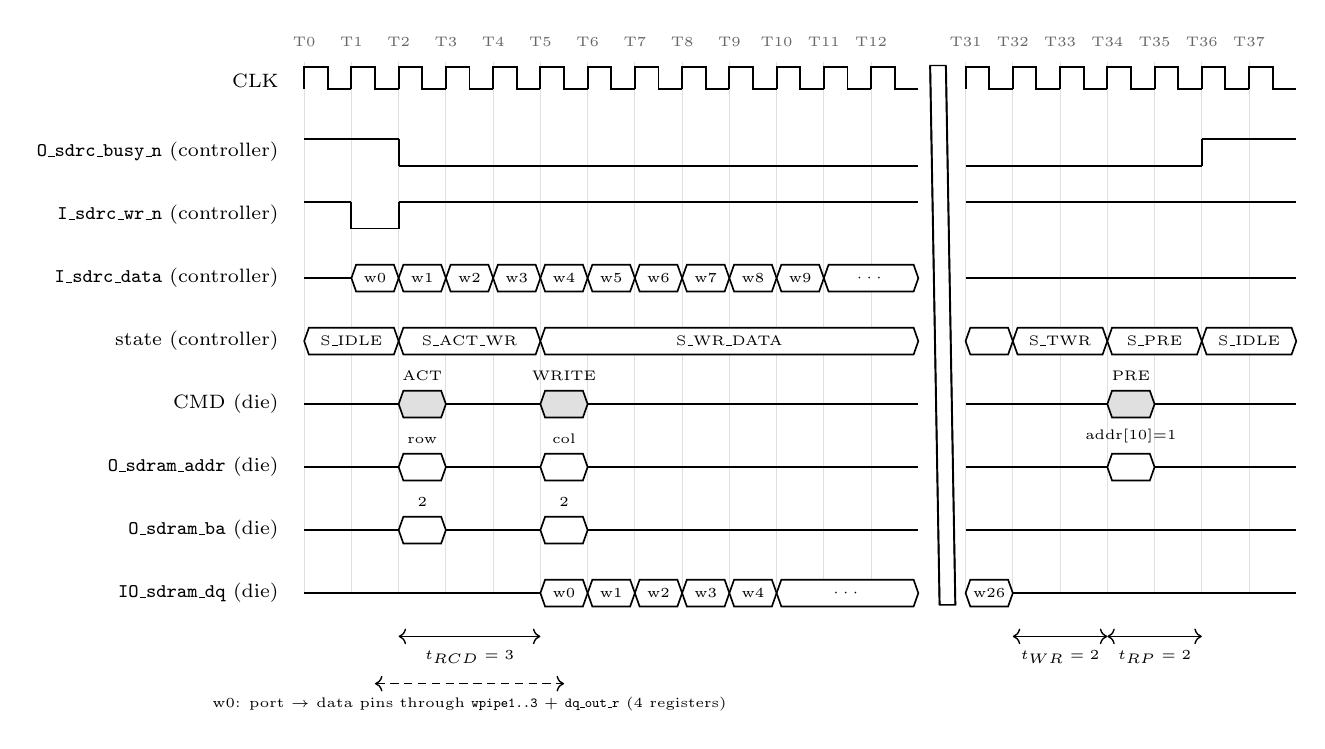
\begin{tikzpicture}[every node/.style={font=\scriptsize}]
\def\XB{8.4}
% ticks and grid
\wticks{0}{12}{0.42}{0}
\wgrid{0}{12}{0.35}{-6.4}
\wticks{\XB}{6}{0.42}{31}
\wgrid{\XB}{6}{0.35}{-6.4}
% CLK
\wlab{CLK}{0.1}
\wclk{0}{13}{0}
\wclk{\XB}{7}{0}
% busy_n
\wlab{\texttt{O\_sdrc\_busy\_n} (controller)}{-0.8}
\whi{0}{1.2}{-0.8}\wfe{1.2}{-0.8}\wlo{1.2}{7.8}{-0.8}
\wlo{\XB}{11.4}{-0.8}\wfe{11.4}{-0.8}\whi{11.4}{12.6}{-0.8}
% wr_n
\wlab{\texttt{I\_sdrc\_wr\_n} (controller)}{-1.6}
\whi{0}{0.6}{-1.6}\wfe{0.6}{-1.6}\wlo{0.6}{1.2}{-1.6}\wfe{1.2}{-1.6}\whi{1.2}{7.8}{-1.6}
\whi{\XB}{12.6}{-1.6}
% I_sdrc_data
\wlab{\texttt{I\_sdrc\_data} (controller)}{-2.4}
\widle{0}{0.6}{-2.4}
\wbus{0.6}{1.2}{-2.4}{w0}
\wbus{1.2}{1.8}{-2.4}{w1}
\wbus{1.8}{2.4}{-2.4}{w2}
\wbus{2.4}{3.0}{-2.4}{w3}
\wbus{3.0}{3.6}{-2.4}{w4}
\wbus{3.6}{4.2}{-2.4}{w5}
\wbus{4.2}{4.8}{-2.4}{w6}
\wbus{4.8}{5.4}{-2.4}{w7}
\wbus{5.4}{6.0}{-2.4}{w8}
\wbus{6.0}{6.6}{-2.4}{w9}
\wbus{6.6}{7.8}{-2.4}{$\cdots$}
\widle{\XB}{12.6}{-2.4}
% state
\wlab{state (controller)}{-3.2}
\wbus{0}{1.2}{-3.2}{S\_IDLE}
\wbus{1.2}{3.0}{-3.2}{S\_ACT\_WR}
\wbus{3.0}{7.8}{-3.2}{S\_WR\_DATA}
\wbus{\XB}{9.0}{-3.2}{}
\wbus{9.0}{10.2}{-3.2}{S\_TWR}
\wbus{10.2}{11.4}{-3.2}{S\_PRE}
\wbus{11.4}{12.6}{-3.2}{S\_IDLE}
% CMD
\wlab{CMD (die)}{-4.0}
\widle{0}{1.2}{-4.0}
\wcmd{1.2}{1.8}{-4.0}{ACT}
\widle{1.8}{3.0}{-4.0}
\wcmd{3.0}{3.6}{-4.0}{WRITE}
\widle{3.6}{7.8}{-4.0}
\widle{\XB}{10.2}{-4.0}
\wcmd{10.2}{10.8}{-4.0}{PRE}
\widle{10.8}{12.6}{-4.0}
% O_sdram_addr
\wlab{\texttt{O\_sdram\_addr} (die)}{-4.8}
\widle{0}{1.2}{-4.8}
\wval{1.2}{1.8}{-4.8}{row}
\widle{1.8}{3.0}{-4.8}
\wval{3.0}{3.6}{-4.8}{col}
\widle{3.6}{7.8}{-4.8}
\widle{\XB}{10.2}{-4.8}
\wval{10.2}{10.8}{-4.8}{addr[10]$=$1}
\widle{10.8}{12.6}{-4.8}
% O_sdram_ba
\wlab{\texttt{O\_sdram\_ba} (die)}{-5.6}
\widle{0}{1.2}{-5.6}
\wval{1.2}{1.8}{-5.6}{2}
\widle{1.8}{3.0}{-5.6}
\wval{3.0}{3.6}{-5.6}{2}
\widle{3.6}{7.8}{-5.6}
\widle{\XB}{10.2}{-5.6}
\widle{10.2}{12.6}{-5.6}
% DQ
\wlab{\texttt{IO\_sdram\_dq} (die)}{-6.4}
\widle{0}{3.0}{-6.4}
\wbus{3.0}{3.6}{-6.4}{w0}
\wbus{3.6}{4.2}{-6.4}{w1}
\wbus{4.2}{4.8}{-6.4}{w2}
\wbus{4.8}{5.4}{-6.4}{w3}
\wbus{5.4}{6.0}{-6.4}{w4}
\wbus{6.0}{7.8}{-6.4}{$\cdots$}
\wbus{\XB}{9.0}{-6.4}{w26}
\widle{9.0}{12.6}{-6.4}
% cut
\wcut{8.05}{0.3}{-6.55}
% brackets
\draw[<->, line width=0.5pt] (1.2,-6.95) -- (3.0,-6.95);
\node[anchor=north, font=\tiny] at (2.1,-7) {$t_{RCD}=3$};
% delay line annotation: w0 from the port (T1) to DQ (T5)
\draw[<->, line width=0.5pt, densely dashed] (0.9,-7.55) -- (3.3,-7.55);
\node[anchor=north, font=\tiny] at (2.1,-7.6)
  {w0: port $\to$ data pins through \texttt{wpipe1..3} $+$ \texttt{dq\_out\_r} (4 registers)};
\draw[<->, line width=0.5pt] (9.0,-6.95) -- (10.2,-6.95);
\node[anchor=north, font=\tiny] at (9.6,-7) {$t_{WR}=2$};
\draw[<->, line width=0.5pt] (10.2,-6.95) -- (11.4,-6.95);
\node[anchor=north, font=\tiny] at (10.8,-7) {$t_{RP}=2$};
\end{tikzpicture}
\caption{Streaming write burst, cycle accurate.}
\label{fig:sdram-write}
\end{figure}

% =====================================================================
\section{The audio pipeline: ADC $\to$ DMA $\to$ FFT $\to$ CPU}
\label{sec:accel}
% =====================================================================

The receive path is two state machines running in parallel with a ping pong buffer
between them, inside the block I call the audio accelerator (\texttt{dma.vhd},
Figure~\ref{fig:audio-zoom}). The capture FSM (\texttt{dma\_proc}, bus master M1)
waits for the SPI master's \texttt{data\_ready\_s} flag (a direct wire, not the bus), reads
the sample over the bus, clears that flag, and writes the sample into \texttt{spi\_raw\_buf},
a $1024\times16$ block RAM holding two 512 sample windows. The FFT FSM
(\texttt{fft\_proc}) takes the window just filled, feeds the Gowin FFT core, collects
the 512 spectrum words into \texttt{fft\_result\_buf}, drains them to SDRAM through
the dedicated write port and raises the frame IRQ. While one half fills, the other
half is processed, so no sample is ever lost. The CPU starts the accelerator once at
boot and never reads a raw sample. The tone decoding runs in firmware, which is the
goal I wanted: do every decision in software.

\begin{figure}[H]
\centering
\resizebox{0.90\textwidth}{!}{%
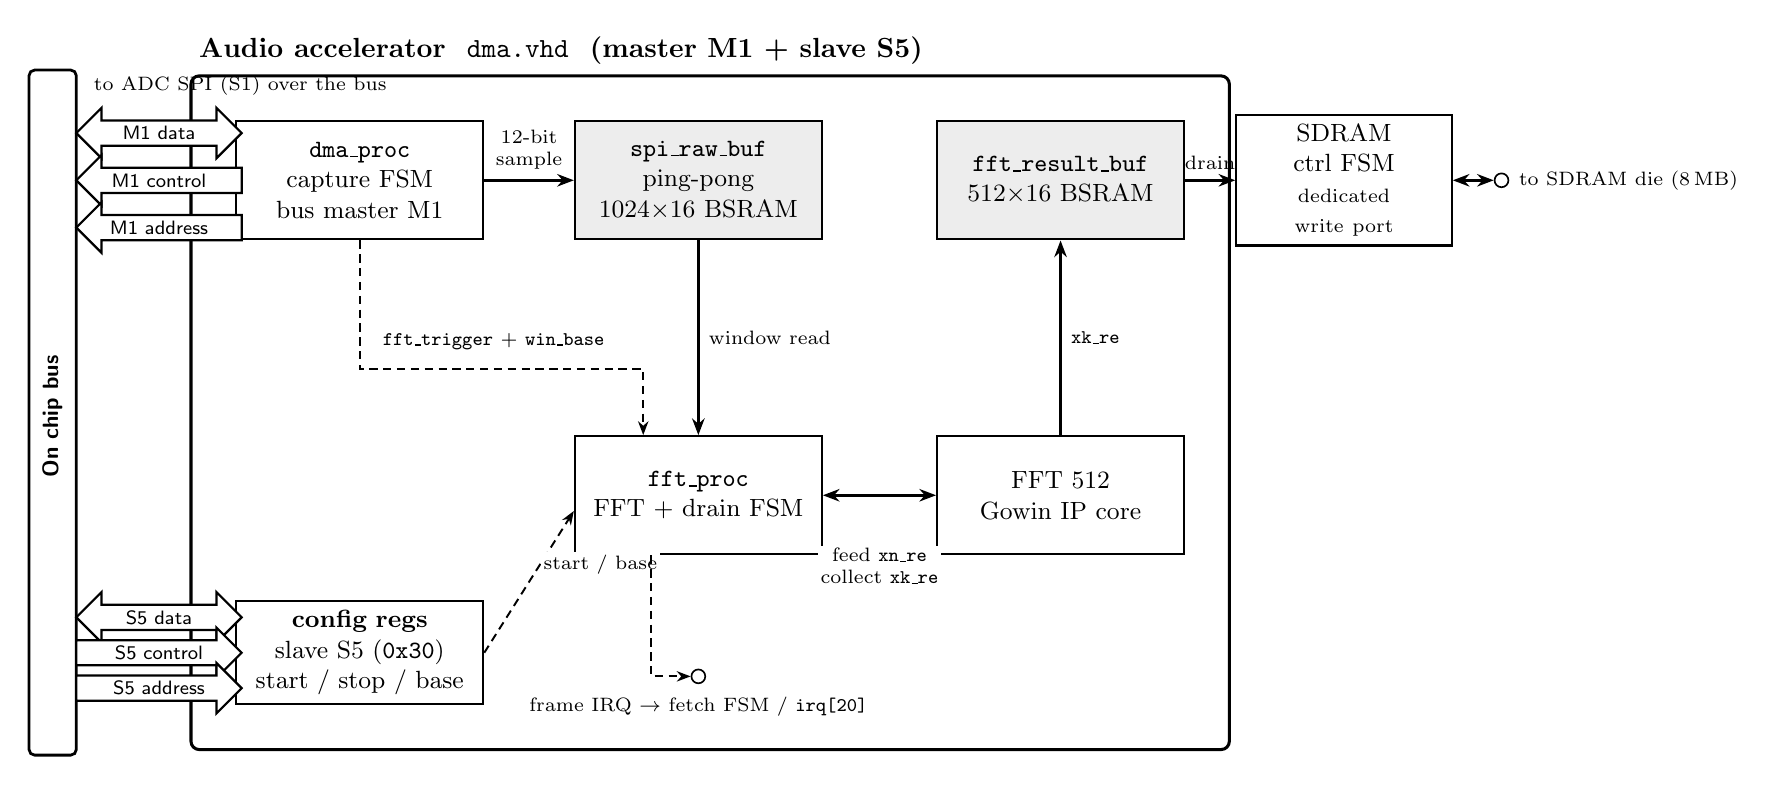
\begin{tikzpicture}[
    every node/.style={font=\small},
    blk/.style={draw, line width=0.8pt, fill=white, minimum width=3.0cm, minimum height=1.5cm, align=center, text width=2.9cm},
    buf/.style={draw, line width=0.8pt, fill=black!7, minimum width=3.0cm, minimum height=1.5cm, align=center, text width=2.9cm},
    sip/.style={draw, line width=0.8pt, fill=white, minimum width=2.6cm, minimum height=1.5cm, align=center, text width=2.5cm},
    pin/.style={circle, draw, fill=white, line width=0.6pt, inner sep=1pt, minimum size=5pt},
    lbl/.style={font=\scriptsize},
    dp/.style={-{Stealth[length=6pt]}, line width=1.0pt},
    dpb/.style={{Stealth[length=6pt]}-{Stealth[length=6pt]}, line width=1.0pt},
    ctl/.style={-{Stealth[length=5pt]}, line width=0.7pt, densely dashed}
]
\newcommand{\zR}[4]{\draw[fill=white, line width=0.8pt]
    (#1,#3+0.16) -- (#2-0.32,#3+0.16) -- (#2-0.32,#3+0.32) -- (#2,#3) --
    (#2-0.32,#3-0.32) -- (#2-0.32,#3-0.16) -- (#1,#3-0.16) -- cycle;
    \node[font=\scriptsize\sffamily] at ($(#1,#3)!0.5!(#2,#3)$) {#4};}
\newcommand{\zL}[4]{\draw[fill=white, line width=0.8pt]
    (#2,#3+0.16) -- (#1+0.32,#3+0.16) -- (#1+0.32,#3+0.32) -- (#1,#3) --
    (#1+0.32,#3-0.32) -- (#1+0.32,#3-0.16) -- (#2,#3-0.16) -- cycle;
    \node[font=\scriptsize\sffamily] at ($(#1,#3)!0.5!(#2,#3)$) {#4};}
\newcommand{\zBi}[4]{\draw[fill=white, line width=0.8pt]
    (#1+0.32,#3+0.16) -- (#2-0.32,#3+0.16) -- (#2-0.32,#3+0.32) -- (#2,#3) --
    (#2-0.32,#3-0.32) -- (#2-0.32,#3-0.16) -- (#1+0.32,#3-0.16) --
    (#1+0.32,#3-0.32) -- (#1,#3) -- (#1+0.32,#3+0.32) -- cycle;
    \node[font=\scriptsize\sffamily] at ($(#1,#3)!0.5!(#2,#3)$) {#4};}
\def\Bx{0.3}\def\Ble{2.4}\def\Sle{2.4}

\draw[fill=white, line width=1.0pt, rounded corners=2pt] (-0.3,-4.7) rectangle (0.3,4.0);
\node[rotate=90, font=\bfseries\sffamily\footnotesize] at (0,-0.4) {On chip bus};

\node[blk] (dma) at (3.9,2.6) {\textbf{\texttt{dma\_proc}}\\capture FSM\\bus master M1};
\node[blk, minimum height=1.2cm] (cfg) at (3.9,-3.4) {\textbf{config regs}\\slave S5 (\texttt{0x30})\\start / stop / base};
\node[buf] (raw) at (8.2,2.6) {\texttt{spi\_raw\_buf}\\ping-pong\\$1024{\times}16$ BSRAM};
\node[blk] (fft) at (8.2,-1.4) {\textbf{\texttt{fft\_proc}}\\FFT + drain FSM};
\node[blk] (core) at (12.8,-1.4) {FFT 512\\Gowin IP core};
\node[buf] (res) at (12.8,2.6) {\texttt{fft\_result\_buf}\\$512{\times}16$ BSRAM};
\node[sip] (sip) at (16.4,2.6) {SDRAM ctrl FSM\\\scriptsize dedicated write port};

\zBi{\Bx}{\Ble}{2.6+0.6}{M1 data}
\zL{\Bx}{\Ble}{2.6}{M1 control}
\zL{\Bx}{\Ble}{2.6-0.6}{M1 address}
\node[lbl, anchor=south west] at (0.4,3.55) {to ADC SPI (S1) over the bus};
\zBi{\Bx}{\Sle}{-3.4+0.45}{S5 data}
\zR{\Bx}{\Sle}{-3.4}{S5 control}
\zR{\Bx}{\Sle}{-3.4-0.45}{S5 address}

\draw[dp] (dma.east) -- node[lbl, above, align=center]{12-bit\\ sample} (raw.west);
\draw[dp] (raw.south) -- node[lbl, right]{window read} (raw.south |- fft.north);
\draw[dpb] (fft.east) -- (core.west);
\node[lbl, align=center, font=\scriptsize, fill=white, inner sep=1pt] at (10.5,-2.3) {feed \texttt{xn\_re}\\collect \texttt{xk\_re}};
\draw[dp] (core.north) -- node[lbl, right]{\texttt{xk\_re}} (core.north |- res.south);
\draw[dp] (res.east) -- node[lbl, above]{drain} (sip.west);

\draw[ctl] (dma.south) |- (5.6,0.2) -| ([xshift=-7mm]fft.north);
\node[lbl, fill=white, inner sep=1pt] at (5.6,0.55) {\texttt{fft\_trigger} + \texttt{win\_base}};
\draw[ctl] (cfg.east) -- node[lbl, pos=0.62, right, fill=white, inner sep=1pt]{start / base} ([yshift=-2mm]fft.west);

\node[pin] (sdpin) at (18.4,2.6){}; \draw[dpb] (sip.east) -- (sdpin);
\node[lbl, anchor=west] at (sdpin.east) {to SDRAM die (8\,MB)};
\node[pin] (irq) at (8.2,-3.7){}; \draw[ctl] ([xshift=-6mm]fft.south) |- (irq);
\node[lbl, anchor=north] at ([yshift=-1pt]irq.south) {frame IRQ $\to$ fetch FSM / \texttt{irq[20]}};

\begin{scope}[on background layer]
\node[draw, line width=1.1pt, fit=(dma)(cfg)(raw)(fft)(core)(res), inner sep=16pt, rounded corners=3pt] (box){};
\end{scope}
\node[anchor=south west, font=\bfseries] at (box.north west) {Audio accelerator \ \texttt{dma.vhd} \ (master M1 + slave S5)};
\end{tikzpicture}%
}
\caption{Audio accelerator block diagram.}
\label{fig:audio-zoom}
\end{figure}

\subsection{The two state machines}

Both are drawn as state diagrams. Each box is a state, with its name and what it does
there (the register updates); each arrow shows the condition that moves the machine to
the next state.

\begin{figure}[H]
\centering
\resizebox{0.97\textwidth}{!}{%
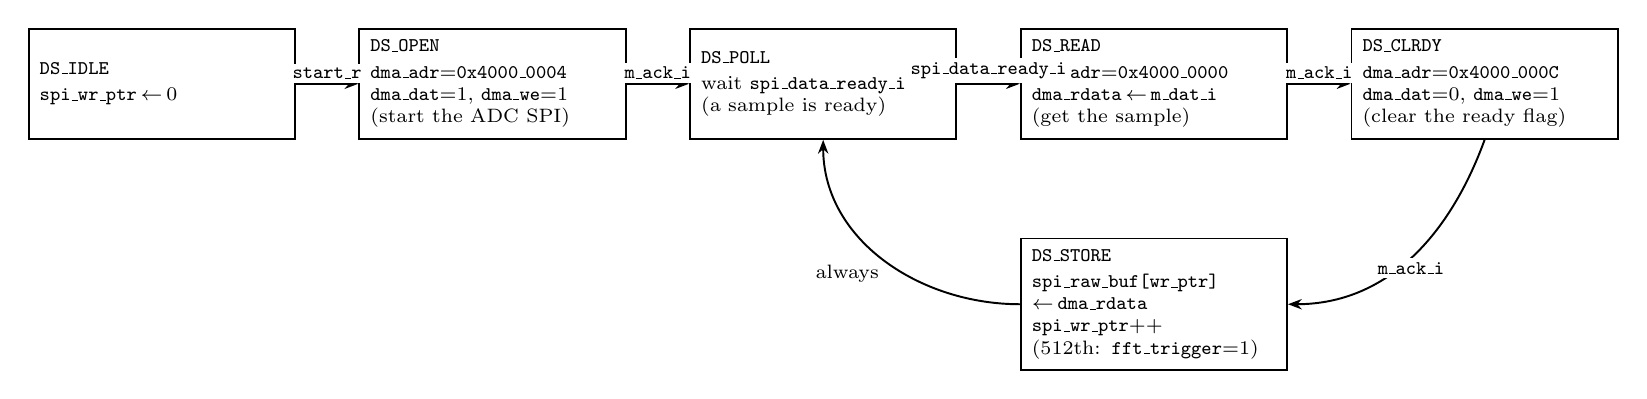
\begin{tikzpicture}[
    every node/.style={font=\footnotesize},
    hb/.style={draw, line width=0.7pt, fill=white, align=left, inner sep=4pt, font=\scriptsize, text width=3.1cm, minimum height=1.4cm},
    a/.style={-{Stealth[length=5pt]}, line width=0.7pt},
    al/.style={font=\scriptsize, fill=white, inner sep=1.5pt}
]
\def\hh#1{\textbf{\texttt{#1}}\\[1.5pt]}
\node[hb] (idle)  at (0,0)     {\hh{DS\_IDLE}\texttt{spi\_wr\_ptr}\,$\leftarrow$\,0};
\node[hb] (open)  at (4.2,0)   {\hh{DS\_OPEN}\texttt{dma\_adr}=\texttt{0x4000\_0004}\\ \texttt{dma\_dat}=1, \texttt{dma\_we}=1\\ (start the ADC SPI)};
\node[hb] (poll)  at (8.4,0)   {\hh{DS\_POLL}wait \texttt{spi\_data\_ready\_i}\\ (a sample is ready)};
\node[hb] (read)  at (12.6,0)  {\hh{DS\_READ}\texttt{dma\_adr}=\texttt{0x4000\_0000}\\ \texttt{dma\_rdata}\,$\leftarrow$\,\texttt{m\_dat\_i}\\ (get the sample)};
\node[hb] (clr)   at (16.8,0)  {\hh{DS\_CLRDY}\texttt{dma\_adr}=\texttt{0x4000\_000C}\\ \texttt{dma\_dat}=0, \texttt{dma\_we}=1\\ (clear the ready flag)};
\node[hb] (store) at (12.6,-2.8){\hh{DS\_STORE}\texttt{spi\_raw\_buf[wr\_ptr]}\\ $\leftarrow$\,\texttt{dma\_rdata}\\ \texttt{spi\_wr\_ptr}++\\ (512th: \texttt{fft\_trigger}=1)};
\draw[a] (idle) -- node[al,above]{\texttt{start\_r}} (open);
\draw[a] (open) -- node[al,above]{\texttt{m\_ack\_i}} (poll);
\draw[a] (poll) -- node[al,above]{\texttt{spi\_data\_ready\_i}} (read);
\draw[a] (read) -- node[al,above]{\texttt{m\_ack\_i}} (clr);
\draw[a] (clr.south)  to[out=250,in=0] node[al,below]{\texttt{m\_ack\_i}} (store.east);
\draw[a] (store.west) to[out=180,in=270] node[al,below left]{always} (poll.south);
\end{tikzpicture}%
}
\caption{Capture FSM (\texttt{dma\_proc}).}
\label{fig:capture-fsm}
\end{figure}

\begin{figure}[H]
\centering
\resizebox{\textwidth}{!}{%
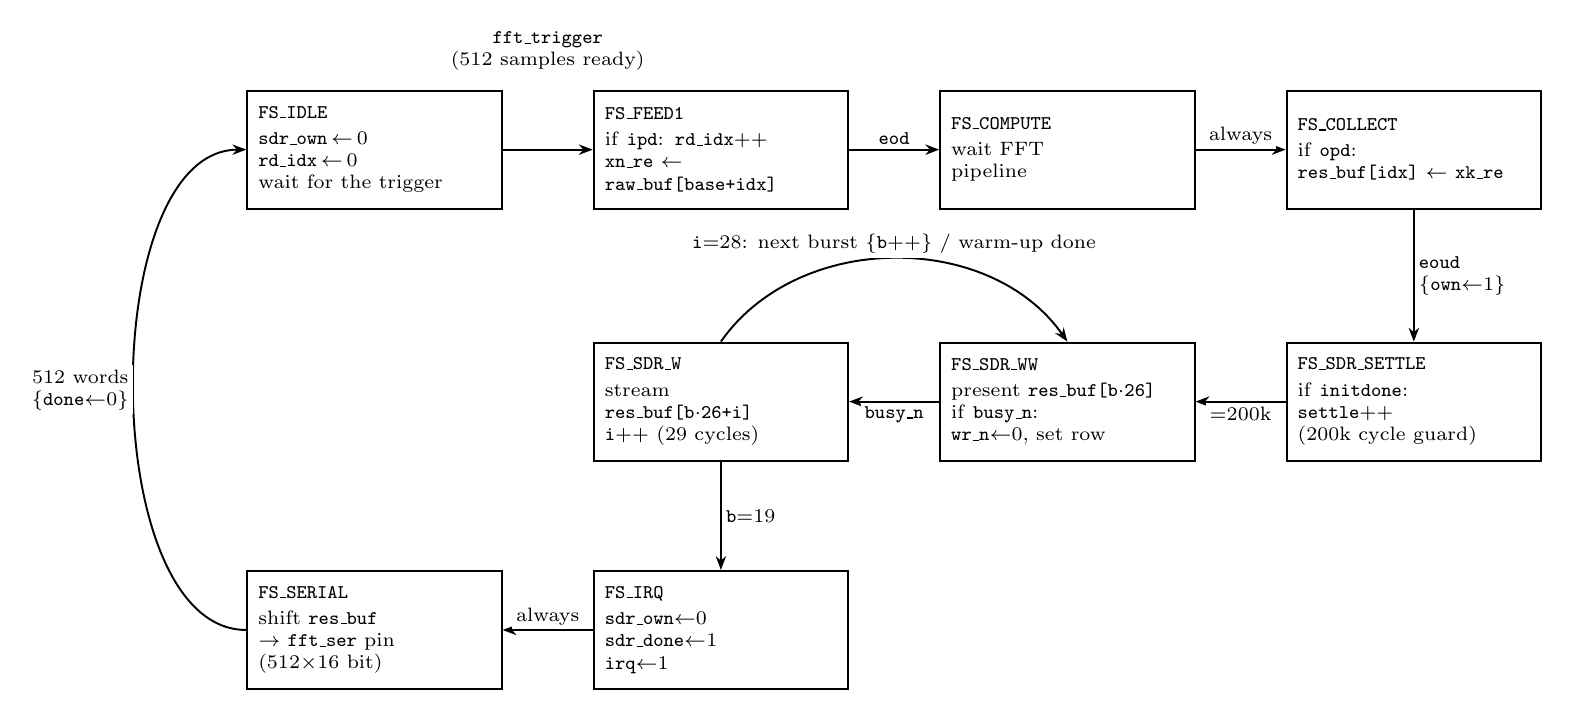
\begin{tikzpicture}[
    every node/.style={font=\footnotesize},
    hb/.style={draw, line width=0.7pt, fill=white, align=left, inner sep=4pt, font=\scriptsize, text width=2.95cm, minimum height=1.5cm},
    a/.style={-{Stealth[length=5pt]}, line width=0.7pt},
    al/.style={font=\scriptsize, fill=white, inner sep=1.5pt}
]
\def\hh#1{\textbf{\texttt{#1}}\\[1.5pt]}
\node[hb] (idle) at (0,0)    {\hh{FS\_IDLE}\texttt{sdr\_own}\,$\leftarrow$\,0\\\texttt{rd\_idx}\,$\leftarrow$\,0\\ wait for the trigger};
\node[hb] (feed) at (4.4,0)  {\hh{FS\_FEED1}if \texttt{ipd}: \texttt{rd\_idx}++\\\texttt{xn\_re} $\leftarrow$\\\texttt{raw\_buf[base+idx]}};
\node[hb] (comp) at (8.8,0)  {\hh{FS\_COMPUTE}wait FFT\\pipeline};
\node[hb] (coll) at (13.2,0) {\hh{FS\_COLLECT}if \texttt{opd}:\\\texttt{res\_buf[idx]} $\leftarrow$ \texttt{xk\_re}};
\node[hb] (settle) at (13.2,-3.2) {\hh{FS\_SDR\_SETTLE}if \texttt{initdone}:\\\texttt{settle}++\\(200k cycle guard)};
\node[hb] (ww) at (8.8,-3.2) {\hh{FS\_SDR\_WW}present \texttt{res\_buf[b$\cdot$26]}\\if \texttt{busy\_n}:\\\texttt{wr\_n}$\leftarrow$0, set row};
\node[hb] (w) at (4.4,-3.2) {\hh{FS\_SDR\_W}stream\\\texttt{res\_buf[b$\cdot$26+i]}\\\texttt{i}++ (29 cycles)};
\node[hb] (irq) at (4.4,-6.1) {\hh{FS\_IRQ}\texttt{sdr\_own}$\leftarrow$0\\\texttt{sdr\_done}$\leftarrow$1\\\texttt{irq}$\leftarrow$1};
\node[hb] (ser) at (0,-6.1) {\hh{FS\_SERIAL}shift \texttt{res\_buf}\\$\to$ \texttt{fft\_ser} pin\\(512$\times$16 bit)};
\node[al,align=center] at (2.2,1.25) {\texttt{fft\_trigger}\\ (512 samples ready)};
\draw[a] (idle) -- (feed);
\draw[a] (feed) -- node[al,above]{\texttt{eod}} (comp);
\draw[a] (comp) -- node[al,above]{always} (coll);
\draw[a] (coll) -- node[al,right,align=left]{\texttt{eoud}\\\{\texttt{own}$\leftarrow$1\}} (settle);
\draw[a] (settle) -- node[al,below]{$=$200k} (ww);
\draw[a] (ww) -- node[al,below]{\texttt{busy\_n}} (w);
\draw[a] (w.north) to[out=55,in=125] node[al,above]{\texttt{i}$=$28: next burst \{\texttt{b}++\} / warm-up done} (ww.north);
\draw[a] (w) -- node[al,right]{\texttt{b}$=$19} (irq);
\draw[a] (irq) -- node[al,above]{always} (ser);
\draw[a] (ser.west) to[out=180,in=180,looseness=0.8] node[al,left,align=center]{512 words\\\{\texttt{done}$\leftarrow$0\}} (idle.west);
\end{tikzpicture}%
}
\caption{FFT and drain FSM (\texttt{fft\_proc}).}
\label{fig:fft-fsm}
\end{figure}

\subsection{The ADC SPI master}
\label{sec:adc}

The analog front end (bottom of Figure~\ref{fig:board}) biases the electret capsule with a 47k/47k divider, amplifies it by $G = 1 + 100\mathrm{k}/10\mathrm{k}
= 11$ in an MCP6022 non inverting configuration, and passes it through a small RC low pass
into the MCP3201. The filter uses a $680\,\Omega$ resistor with the 102 (1\,nF) capacitors,
so
$f_c = 1/(2\pi \cdot 680\,\Omega \cdot 1\,\mathrm{nF}) = 234$\,kHz; it only trims fast noise.
A tight anti alias filter is not needed here because the protocol tones (2 to 4577\,Hz) sit
far below Nyquist ($f_s/2=23.4$\,kHz), and the electret and the amplifier already roll off
well before it. The MCP3201 is a 12 bit SAR ADC that the FPGA reads over SPI with a
dedicated master (\texttt{spi\_master.vhd}); its internal block diagram
is in Figure~\ref{fig:mcp3201-block}.

The master runs off the 40.5\,MHz clock and makes one SCK every 54 clock cycles:
\[
f_\mathrm{SCK} = \frac{40.5\ \mathrm{MHz}}{54} = 750\ \mathrm{kHz}.
\]
A frame is 16 SCK, so it takes $16 \times 54 = 864$ clock cycles $= 21.33\,\mu$s, and the
sample rate is $f_s = 1/(21.33\,\mu\mathrm{s}) = 46.875$\,kHz. The frame is simple: CS goes
low, the ADC sends one null bit and then the 12 data bits MSB first, and after the data CS
goes high for 2 SCK and the frame starts again. Nothing is sent to the ADC, so
\texttt{MOSI} is unused.

The FSM has three states: \texttt{S\_SHIFT} covers bit periods 0 to 13 with CS low (the 12
data bits are captured on periods 2 to 13), \texttt{S\_GAP} covers periods 14 to 15 with
CS high, and while the start register stays set the machine loops
\texttt{S\_GAP}$\to$\texttt{S\_SHIFT} with no dead cycle. When the frame ends
\texttt{data\_ready\_s} goes to 1. The FSM is in
Figure~\ref{fig:spi-timing}, and one frame cycle by cycle is in Figure~\ref{fig:spi-wave}.


\begin{figure}[H]
\centering
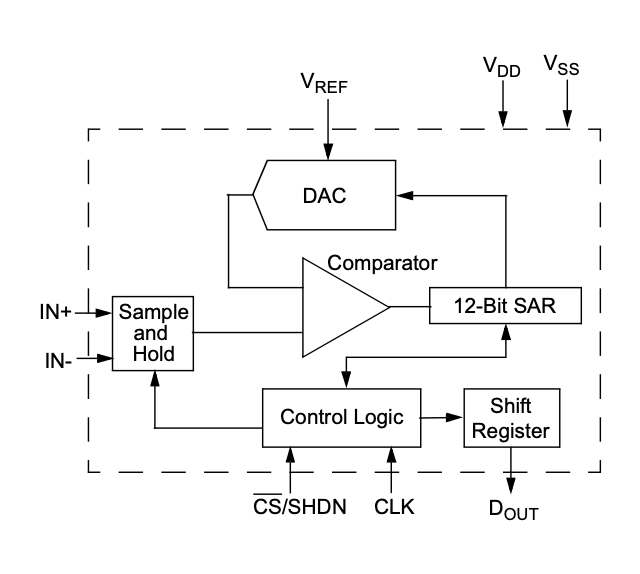
\includegraphics[width=0.52\linewidth]{img/spi_adc_circuit.png}
\caption{MCP3201 internal block diagram.}
\label{fig:mcp3201-block}
\end{figure}


\begin{figure}[H]
\centering
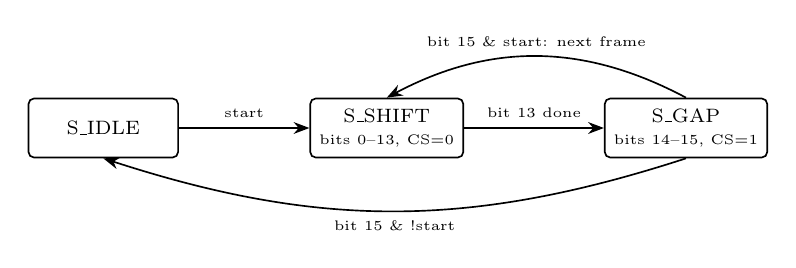
\begin{tikzpicture}[every node/.style={font=\scriptsize}]
\tikzset{stx/.style={rounded corners=2pt, draw, line width=0.6pt, fill=white, minimum width=1.9cm, minimum height=0.75cm, align=center, font=\scriptsize}}
\node[stx] (i) at (0,0) {S\_IDLE};
\node[stx] (s) at (3.6,0) {S\_SHIFT\\ \tiny bits 0--13, CS$=$0};
\node[stx] (g) at (7.4,0) {S\_GAP\\ \tiny bits 14--15, CS$=$1};
\draw[-{Stealth}, line width=0.6pt] (i) -- node[font=\tiny, above]{start} (s);
\draw[-{Stealth}, line width=0.6pt] (s) -- node[font=\tiny, above]{bit 13 done} (g);
\draw[-{Stealth}, line width=0.6pt] (g.north) to[bend right=28] node[font=\tiny, above]{bit 15 \& start: next frame} (s.north);
\draw[-{Stealth}, line width=0.6pt] (g.south) to[bend left=18] node[font=\tiny, below]{bit 15 \& !start} (i.south);
\end{tikzpicture}
\caption{ADC SPI master FSM (\texttt{spi\_master.vhd}).}
\label{fig:spi-timing}
\end{figure}

\begin{figure}[H]
\centering
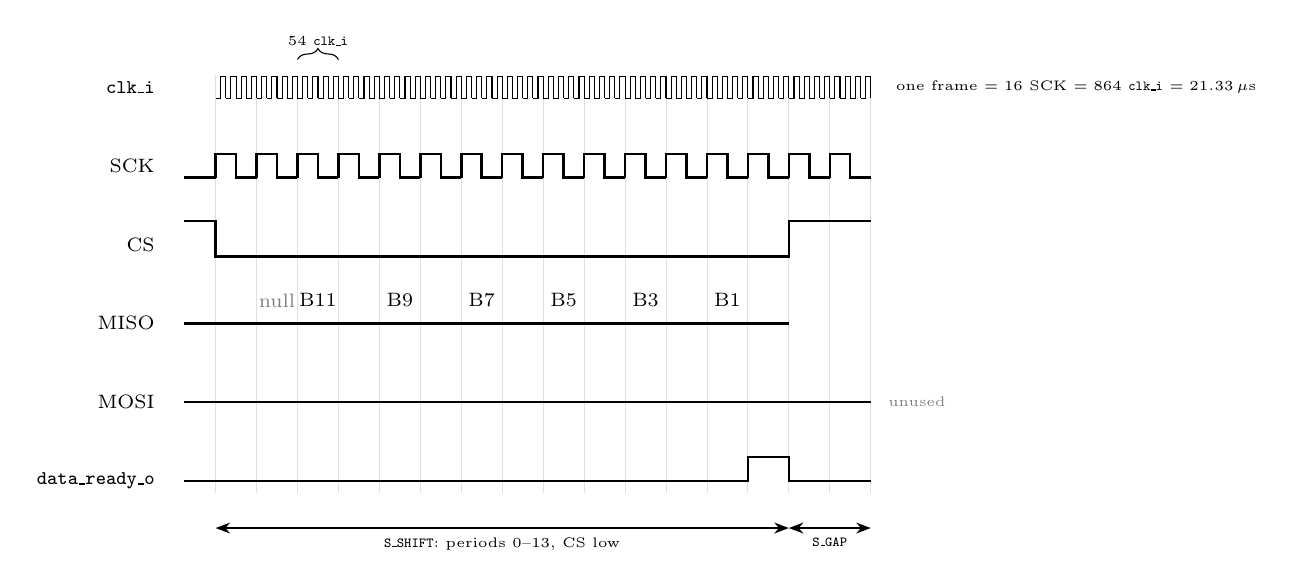
\begin{tikzpicture}[every node/.style={font=\scriptsize}, sig/.style={line width=0.9pt}, >={Stealth}]
\def\T{0.52}
\node[anchor=east] at (-0.25, 3.0) {\texttt{clk\_i}};
\node[anchor=east] at (-0.25, 2.0) {SCK};
\node[anchor=east] at (-0.25, 1.0) {CS};
\node[anchor=east] at (-0.25, 0.0) {MISO};
\node[anchor=east] at (-0.25,-1.0) {MOSI};
\node[anchor=east] at (-0.25,-2.0) {\texttt{data\_ready\_o}};
% vertical grid tied to SCK
\sgrid{0.4}{16}{\T}{3.15}{-2.15}
% clk_i continuous across the whole frame
\clkspan{0.4}{0.4+16*\T}{3.0}{0.13}
\draw[decorate,decoration={brace,amplitude=4pt},line width=0.4pt] ({0.4+2*\T},3.35) -- ({0.4+3*\T},3.35);
\node[anchor=south,font=\tiny] at ({0.4+2.5*\T},3.4) {$54$ \texttt{clk\_i}};
\node[anchor=west,font=\tiny] at ({0.4+16*\T+0.2},3.0) {one frame $=16$ SCK $=864$ \texttt{clk\_i} $=21.33\,\mu$s};
% SCK
\draw[sig] (0,1.85) -- (0.4,1.85);
\foreach \i in {0,...,15}{
  \draw[sig] ({0.4+\i*\T},1.85) -- ({0.4+\i*\T},2.15) -- ({0.4+\i*\T+0.5*\T},2.15) -- ({0.4+\i*\T+0.5*\T},1.85) -- ({0.4+\i*\T+\T},1.85);}
% CS
\draw[sig] (0,1.3) -- (0.4,1.3) -- (0.4,0.85) -- ({0.4+14*\T},0.85) -- ({0.4+14*\T},1.3) -- ({0.4+16*\T},1.3);
% MISO: null then 12 data bits
\draw[sig] (0,0.0) -- ({0.4+14*\T},0.0);
\node[gray] at ({0.4+1.5*\T},0.28){null};
\foreach \i/\b in {0/{B11},2/{B9},4/{B7},6/{B5},8/{B3},10/{B1}}{
  \node at ({0.4+(2.5+\i)*\T},0.3){\b};}
% MOSI unused
\draw[sig] (0,-1.0) -- ({0.4+16*\T},-1.0);
\node[gray, anchor=west, font=\tiny] at ({0.4+16*\T+0.1},-1.0){unused};
% data_ready_o pulse
\draw[sig] (0,-2.0) -- ({0.4+13*\T},-2.0) -- ({0.4+13*\T},-1.7) -- ({0.4+14*\T},-1.7) -- ({0.4+14*\T},-2.0) -- ({0.4+16*\T},-2.0);
% S_SHIFT / S_GAP at the bottom
\draw[<->, line width=0.5pt] (0.4,-2.6) -- ({0.4+14*\T},-2.6);
\node[anchor=north, font=\tiny] at ({0.4+7*\T},-2.6){\texttt{S\_SHIFT}: periods 0--13, CS low};
\draw[<->, line width=0.5pt] ({0.4+14*\T},-2.6) -- ({0.4+16*\T},-2.6);
\node[anchor=north, font=\tiny] at ({0.4+15*\T},-2.6){\texttt{S\_GAP}};
\end{tikzpicture}
\caption{One MCP3201 frame, cycle by cycle. \texttt{MOSI} is unused; the 12 data bits arrive MSB first on \texttt{MISO}.}
\label{fig:spi-wave}
\end{figure}

\subsection{Timing of the whole chain}
\label{sec:pipeline}

The ADC sets the timing of the whole chain: one sample every $864$ cycles ($21.33\,\mu$s),
one window of 512 samples every
\[
t_\mathrm{window} = 16\times512\times54 = 442\,368\ \mathrm{cycles} = 10.92\ \mathrm{ms}
\quad\Rightarrow\quad 91.6\ \mathrm{frames/s},\qquad
\Delta f = \frac{46\,875}{512} = 91.6\ \mathrm{Hz\ per\ bin}.
\]
Processing one window costs about $37\,\mu$s of FFT feed/collect, a 
$4.94$\,ms wait before the first SDRAM write 200\,000 cycles, $25\,\mu$s of drain (21 bursts) and $202\,\mu$s of serial debug stream:
\[
t_\mathrm{process} = 5.2\ \mathrm{ms} < t_\mathrm{window} = 10.92\ \mathrm{ms}.
\]
The ping pong buffer is what lets capture and processing run at the same time
(Figure~\ref{fig:pipeline}). Almost all of $t_\mathrm{process}$ is that wait before the
SDRAM write.

% waveform helpers for the capture timing diagram
\newcommand{\pclk}[4]{%
  \foreach \i in {1,...,#2}{%
    \draw[line width=0.5pt]
      ({#1+(\i-1)*#3},{#4-0.16}) -- ({#1+(\i-1)*#3},{#4+0.16})
      -- ({#1+(\i-1)*#3+0.5*#3},{#4+0.16}) -- ({#1+(\i-1)*#3+0.5*#3},{#4-0.16})
      -- ({#1+(\i-1)*#3+#3},{#4-0.16});}}
\newcommand{\pbus}[4]{%
  \draw[line width=0.6pt] ({#1},{#3+0.2}) -- ({#2},{#3+0.2});
  \draw[line width=0.6pt] ({#1},{#3-0.2}) -- ({#2},{#3-0.2});
  \draw[line width=0.6pt] ({#1},{#3-0.2}) -- ({#1},{#3+0.2});
  \draw[line width=0.6pt] ({#2},{#3-0.2}) -- ({#2},{#3+0.2});
  \node[font=\tiny] at ({(#1+#2)/2},{#3}) {#4};}
\newcommand{\plow}[3]{\draw[line width=0.7pt] ({#1},{#3-0.2}) -- ({#2},{#3-0.2});}
\newcommand{\phigh}[3]{\draw[line width=0.7pt] ({#1},{#3+0.2}) -- ({#2},{#3+0.2});}
\newcommand{\pcut}[3]{%
  \draw[white, line width=4pt] ({#1},{#2}) -- ({#1},{#3});
  \draw[line width=0.5pt] ({#1-0.14},{#2}) -- ({#1+0.02},{#3});
  \draw[line width=0.5pt] ({#1+0.10},{#2}) -- ({#1+0.26},{#3});}
\begin{figure}[H]
\centering
\resizebox{\textwidth}{!}{%
\begin{tikzpicture}[every node/.style={font=\scriptsize}]
\def\yclk{0}
\def\ysck{-0.9}
\def\ycs{-1.8}
\def\ymiso{-2.7}
\def\ymosi{-3.6}
\def\yrdy{-4.5}
\def\ystate{-5.8}
\def\yadr{-6.9}
\def\yack{-8.0}
\def\yrdat{-9.0}
\def\yptr{-10.1}
\def\ytrig{-11.2}
% row labels
\node[anchor=east] at (-0.15,\yclk) {\texttt{clk\_i} (40.5\,MHz)};
\node[anchor=east] at (-0.15,\ysck) {SCK};
\node[anchor=east] at (-0.15,\ycs) {CS};
\node[anchor=east] at (-0.15,\ymiso) {MISO};
\node[anchor=east] at (-0.15,\ymosi) {MOSI};
\node[anchor=east] at (-0.15,\yrdy) {\texttt{spi\_data\_ready\_i}};
\node[anchor=east] at (-0.15,\ystate) {\texttt{dma\_curr\_state}};
\node[anchor=east] at (-0.15,\yadr) {\texttt{dma\_adr}};
\node[anchor=east] at (-0.15,\yack) {\texttt{m\_ack\_i}};
\node[anchor=east] at (-0.15,\yrdat) {\texttt{dma\_rdata}};
\node[anchor=east] at (-0.15,\yptr) {\texttt{spi\_wr\_ptr}};
\node[anchor=east] at (-0.15,\ytrig) {\texttt{fft\_trigger}};
% vertical grid tied to SCK inside the two SPI frames
\sgrid{0.3}{4}{0.6}{0.15}{-11.45}\sgrid{4.3}{4}{0.6}{0.15}{-11.45}
\sgrid{11.7}{4}{0.6}{0.15}{-11.45}\sgrid{15.7}{4}{0.6}{0.15}{-11.45}
\node[font=\tiny, anchor=south] at (3.25,0.35) {one frame: 16 SCK $=864$ \texttt{clk\_i} (54 per SCK)};
% ===== word 0: SPI frame =====
\pclk{0.3}{6}{0.3}{\yclk}\pcut{2.7}{\yclk-0.2}{\yclk+0.2}\pclk{4.3}{6}{0.3}{\yclk}
\pclk{0.3}{3}{0.6}{\ysck}\pcut{2.7}{\ysck-0.2}{\ysck+0.2}\pclk{4.3}{3}{0.6}{\ysck}
\draw[line width=0.7pt] (0.0,\ycs+0.2) -- (0.3,\ycs+0.2) -- (0.3,\ycs-0.2) -- (6.2,\ycs-0.2);
\pbus{0.3}{1.1}{\ymiso}{null}\pbus{1.1}{1.9}{\ymiso}{B11}\pbus{1.9}{2.5}{\ymiso}{B10}
\pcut{2.7}{\ymiso-0.2}{\ymiso+0.2}\pbus{4.3}{5.2}{\ymiso}{B1}\pbus{5.2}{6.2}{\ymiso}{B0}
\plow{0.0}{6.2}{\ymosi}
\node[gray,font=\tiny,anchor=south] at (3.1,\ymosi-0.18) {unused};
\draw[line width=0.7pt] (0.0,\yrdy-0.2) -- (6.2,\yrdy-0.2) -- (6.2,\yrdy+0.2);
\pbus{0.3}{6.2}{\ystate}{\texttt{DS\_POLL}}
\plow{0.0}{6.2}{\yadr}\plow{0.0}{6.2}{\yack}
\pbus{0.3}{6.2}{\yrdat}{--}\pbus{0.3}{6.2}{\yptr}{0}\plow{0.0}{6.2}{\ytrig}
% ===== word 0: DMA read/store =====
\pclk{6.2}{14}{0.3}{\yclk}
\plow{6.2}{10.6}{\ysck}
\phigh{6.2}{10.6}{\ycs}\draw[line width=0.7pt](6.2,\ycs-0.2)--(6.2,\ycs+0.2);
\plow{6.2}{10.6}{\ymiso}\plow{6.2}{10.6}{\ymosi}
\draw[line width=0.7pt] (6.2,\yrdy+0.2) -- (9.2,\yrdy+0.2) -- (9.2,\yrdy-0.2) -- (10.6,\yrdy-0.2);
\pbus{6.2}{7.9}{\ystate}{\texttt{DS\_READ}}\pbus{7.9}{9.4}{\ystate}{\texttt{DS\_CLRDY}}\pbus{9.4}{10.6}{\ystate}{\texttt{DS\_STORE}}
\pbus{6.2}{7.9}{\yadr}{\texttt{0x4000\_0000}}\pbus{7.9}{9.4}{\yadr}{\texttt{0x4000\_000C}}\plow{9.4}{10.6}{\yadr}
\draw[line width=0.7pt]
 (6.2,\yack-0.2) -- (7.4,\yack-0.2) -- (7.4,\yack+0.2) -- (7.9,\yack+0.2) -- (7.9,\yack-0.2)
 -- (8.9,\yack-0.2) -- (8.9,\yack+0.2) -- (9.4,\yack+0.2) -- (9.4,\yack-0.2) -- (10.6,\yack-0.2);
\pbus{6.2}{7.9}{\yrdat}{--}\pbus{7.9}{10.6}{\yrdat}{\texttt{0x0AB}}
\pbus{6.2}{9.9}{\yptr}{0}\pbus{9.9}{10.6}{\yptr}{1}\plow{6.2}{10.6}{\ytrig}
% ===== big cut =====
\foreach \yy in {\yclk,\ysck,\ycs,\ymiso,\ymosi,\yrdy,\ystate,\yadr,\yack,\yrdat,\yptr,\ytrig}{
  \pcut{11.1}{\yy-0.22}{\yy+0.22}}
\node[font=\tiny, rotate=90] at (11.35,-5.5) {words 1 .. 510 skipped};
% ===== word 511: SPI frame =====
\pclk{11.7}{6}{0.3}{\yclk}\pcut{14.1}{\yclk-0.2}{\yclk+0.2}\pclk{15.7}{6}{0.3}{\yclk}
\pclk{11.7}{3}{0.6}{\ysck}\pcut{14.1}{\ysck-0.2}{\ysck+0.2}\pclk{15.7}{3}{0.6}{\ysck}
\draw[line width=0.7pt] (11.0,\ycs+0.2) -- (11.7,\ycs+0.2) -- (11.7,\ycs-0.2) -- (17.6,\ycs-0.2);
\pbus{11.7}{12.5}{\ymiso}{null}\pbus{12.5}{13.3}{\ymiso}{B11}\pbus{13.3}{13.9}{\ymiso}{B10}
\pcut{14.1}{\ymiso-0.2}{\ymiso+0.2}\pbus{15.7}{16.6}{\ymiso}{B1}\pbus{16.6}{17.6}{\ymiso}{B0}
\plow{11.0}{17.6}{\ymosi}
\draw[line width=0.7pt] (11.0,\yrdy-0.2) -- (17.6,\yrdy-0.2) -- (17.6,\yrdy+0.2);
\pbus{11.7}{17.6}{\ystate}{\texttt{DS\_POLL}}
\plow{11.0}{17.6}{\yadr}\plow{11.0}{17.6}{\yack}
\pbus{11.7}{17.6}{\yrdat}{--}\pbus{11.7}{17.6}{\yptr}{511}\plow{11.0}{17.6}{\ytrig}
% ===== word 511: DMA read/store + fft_trigger =====
\pclk{17.6}{14}{0.3}{\yclk}
\plow{17.6}{22.0}{\ysck}
\phigh{17.6}{22.0}{\ycs}\draw[line width=0.7pt](17.6,\ycs-0.2)--(17.6,\ycs+0.2);
\plow{17.6}{22.0}{\ymiso}\plow{17.6}{22.0}{\ymosi}
\draw[line width=0.7pt] (17.6,\yrdy+0.2) -- (20.6,\yrdy+0.2) -- (20.6,\yrdy-0.2) -- (22.0,\yrdy-0.2);
\pbus{17.6}{19.3}{\ystate}{\texttt{DS\_READ}}\pbus{19.3}{20.8}{\ystate}{\texttt{DS\_CLRDY}}\pbus{20.8}{22.0}{\ystate}{\texttt{DS\_STORE}}
\pbus{17.6}{19.3}{\yadr}{\texttt{0x4000\_0000}}\pbus{19.3}{20.8}{\yadr}{\texttt{0x4000\_000C}}\plow{20.8}{22.0}{\yadr}
\draw[line width=0.7pt]
 (17.6,\yack-0.2) -- (18.8,\yack-0.2) -- (18.8,\yack+0.2) -- (19.3,\yack+0.2) -- (19.3,\yack-0.2)
 -- (20.3,\yack-0.2) -- (20.3,\yack+0.2) -- (20.8,\yack+0.2) -- (20.8,\yack-0.2) -- (22.0,\yack-0.2);
\pbus{17.6}{19.3}{\yrdat}{--}\pbus{19.3}{22.0}{\yrdat}{\texttt{0x1C7}}
\pbus{17.6}{21.3}{\yptr}{511}\pbus{21.3}{22.0}{\yptr}{512}
\draw[line width=0.7pt] (17.6,\ytrig-0.2) -- (21.3,\ytrig-0.2) -- (21.3,\ytrig+0.2) -- (22.0,\ytrig+0.2);
\node[font=\tiny, anchor=south] at (21.6,\ytrig+0.22) {window ready};
% device brackets
\draw[decorate, decoration={brace, amplitude=5pt}] (-3.05,\yclk+0.25) -- (-3.05,\yrdy-0.25);
\node[rotate=90, anchor=south, font=\scriptsize] at (-3.25,{(\yclk+\yrdy)/2}) {SPI Master (\texttt{spi\_master.vhd})};
\draw[decorate, decoration={brace, amplitude=5pt}] (-3.05,\ystate+0.25) -- (-3.05,\ytrig-0.25);
\node[rotate=90, anchor=south, font=\scriptsize] at (-3.25,{(\ystate+\ytrig)/2}) {DMA (\texttt{dma\_proc})};
% column headers
\node[font=\small, anchor=south] at (5.4,0.9) {word 0 capture};
\node[font=\small, anchor=south] at (16.8,0.9) {word 511 capture (window handoff)};
\draw[line width=0.4pt] (0.3,0.75) -- (10.6,0.75);
\draw[line width=0.4pt] (11.7,0.75) -- (22.0,0.75);
\end{tikzpicture}%
}
\caption{Capture of one 512 sample window, cycle by cycle}
\label{fig:pipeline}
\end{figure}

\subsection{Fetch FSM and snapshot}
\label{sec:fetch}

The read side of the SDRAM port is the \emph{fetch FSM}
(Figure~\ref{fig:fetch-fsm}). The frame IRQ does not interrupt the CPU: in hardware
it starts the fetch, which for each of the 20 bursts waits for the controller,
requests a read with that burst's row address, and collects the 26 words into a
$512\times16$ BSRAM. The write side maps each valid word to a fixed bin:
\[
\text{bin} = \texttt{b}\times26 + \texttt{idx}, \qquad
\texttt{b}=0\ldots19\ \text{(20 bursts)}, \quad
\texttt{idx}=0\ldots25\ \text{(26 words)},
\]
The 20 bursts give $20\times26=520$ words, 8 more than
the 512 bin BSRAM, so a \texttt{bin}$<512$ guard keeps bins 0 to 511 and drops the last 8
words of burst 19. When burst 19 finishes, \texttt{fill\_cnt} increments. Each burst runs
The whole fetch is $20\times200=4000$ cycles (about
$100\,\mu$s) of the 10.92\,ms frame.

The fetch fills this snapshot BSRAM, which the CPU reads.
\texttt{fill\_cnt} is how the CPU knows a new spectrum is ready: it is a counter that
goes up by one each time a fetch finishes, and wraps around.
The CPU keeps the last value it read and
compares: when \texttt{fill\_cnt} has changed, a fresh 512 word snapshot is ready and
the CPU copies it through the Wishbone bus.

\begin{figure}[H]
\centering
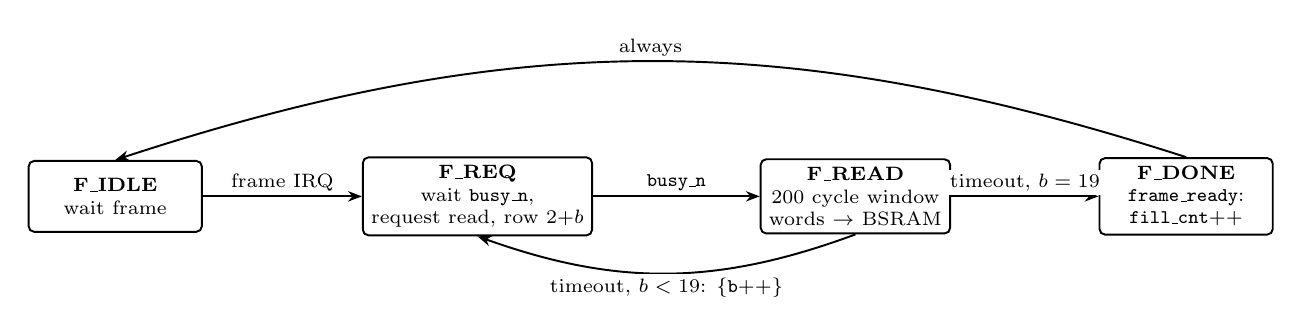
\begin{tikzpicture}[
    every node/.style={font=\footnotesize},
    st/.style={rounded corners=2pt, draw, line width=0.7pt, fill=white, minimum width=2.2cm, minimum height=0.9cm, align=center, inner sep=3pt, font=\scriptsize},
    a/.style={-{Stealth[length=5pt]}, line width=0.7pt},
    al/.style={font=\scriptsize, fill=white, inner sep=1.5pt}
]
\node[st] (idle) at (0,0)    {\textbf{F\_IDLE}\\wait frame};
\node[st] (req)  at (4.6,0)  {\textbf{F\_REQ}\\wait \texttt{busy\_n},\\request read, row $2{+}b$};
\node[st] (read) at (9.4,0)  {\textbf{F\_READ}\\200 cycle window\\words $\to$ BSRAM};
\node[st] (done) at (13.6,0) {\textbf{F\_DONE}\\\texttt{frame\_ready}:\\\texttt{fill\_cnt}++};
\draw[a] (idle) -- node[al,above]{frame IRQ} (req);
\draw[a] (req) -- node[al,above]{\texttt{busy\_n}} (read);
\draw[a] (read.south) to[bend left=20] node[al,below]{timeout, $b<19$: \{\texttt{b}++\}} (req.south);
\draw[a] (read) -- node[al,above]{timeout, $b=19$} (done);
\draw[a] (done.north) to[bend right=18] node[al,above]{always} (idle.north);
\end{tikzpicture}
\caption{Fetch FSM.}
\label{fig:fetch-fsm}
\end{figure}

\subsection{The tone decoder}

The decoder run in C on the soft core, it apply three tests to each of the five
protocol bins: a \emph{local maximum} test against the six neighbours within $\pm3$
bins, a
\emph{curvature} test on $k{-}1,k,k{+}1$ (the peak must open downward, so $k$ is a
crest and not the skirt of a neighbour); and an \emph{amplitude} test on the
parabolically interpolated peak against a fixed threshold exactly how my thesis described. 

% =====================================================================
\section{Tone output}
\label{sec:speaker}
% =====================================================================

The tone output is a Sinusoidal PWM (\texttt{pwm\_generic\_master.vhd}). A free running 8 bit counter
(\texttt{pwm\_cnt\_s}) and a comparator drive the pin: \texttt{PWM\_o} is high while
\texttt{pwm\_cnt\_s} $<$ \texttt{duty\_env\_s}, so the pulse width is set by an 8 bit duty
(0 to 255). The PWM period is $f_\mathrm{clk}/2^{8} = 40.5\,\mathrm{MHz}/256 = 158.2$\,kHz
for the speaker, far above the
audio band.

To guarantee spectral purity, 
I avoided generating a simple square wave because 
it also carries strong odd harmonics at $3f$, $5f$, $7f$ and so on. 
For a tone at $f=2472$\,Hz these harmonics all fall 
below Nyquist ($f_s/2=23.4$\,kHz), so on the receiver they land in other FFT
bins and read as tones that were never sent.

To solve this, I implemented a PWM approach that moves the switching
 far away: the pin still toggles like a square, but at the fixed 158.2\,kHz 
 carrier, and the tone is carried by the \emph{duty}.
  The duty traces a sine from the DDS and the \texttt{SINE\_LUT} 
  (Figure~\ref{fig:spwm}), and the speaker cannot follow 158.2\,kHz
  (its inductance and inertia average the pulses), so it plays back a 
  clean sine at $f$. The unwanted energy now sits at 158.2\,kHz and its 
  multiples, which the speaker does not reproduce, so the audio band hold
   only the wanted tone.



When the module receives the address \texttt{0x04} from the bus, it loads
 two 16-bit frequency values. Each frequency controls its own 24-bit phase
  accumulator. To find out how big the phase step ($\Delta\phi$) should be, 
  FPGAs can't be synthetized with 
  hardware divisions, so I used a math trick that I found in online
   DSP tutorials (using a precomputed constant and
    bit-shifting as explained in \url{https://electronics.stackexchange.com/questions/55493/fixed-point-division-in-verilog-for-spartan-6})
    \newline
    Instead of dividing by the clock frequency, I multiply by a precalculated 
    constant $K$ and then shift the bits to the right. In my code, this is 
    calculated as $(f\cdot K + 2^{23})\gg24$.
\newline

At every single 40.5\,MHz clock tick (the speaker PWM runs on the bus clock), both 24-bit
 accumulators add their specific step ($\Delta\phi$) to their running total.
 However, the \texttt{SINE\_LUT} only has 256 entries, meaning it 
 only needs an 8-bit index to be read ($2^8 = 256$). 
 Therefore, the system takes only the top 8 bits of each 24-bit
 accumulator to find the right position inside the table;
 the lower 16 bits are basically kept as a "fractional" part
  for precision. This is the whole reason the accumulator is 24 bit and not 8: the top 8
  bits only pick which sine sample to read, while the full 24 bit width sets how finely the
  frequency can be tuned. The frequency step is $f_\mathrm{clk}/2^{24}$, a few Hz; with only
  8 bits the smallest step would be $f_\mathrm{clk}/2^{8}$, which is the 158\,kHz carrier
  itself, far too coarse for an audio tone. Since FPGA hardware can run parallel tasks,
  the code actually reads two different values from the exact 
  same table at the exact same time. To send these two different
   frequencies to a single output pin, the code simply adds the two
    retrieved sine values together and divides the result by 2 
    (by doing a simple 1-bit right shift). 
    This creates a single 8-bit mixed duty cycle without overflowing.

Finally, to make the audio sound good, the amplitude is never switched on or off abruptly. If I did that, the speaker would produce a loud clicking noise. Instead, I created a state machine that acts as a volume envelope (states E\_IDLE, E\_ATTACK, E\_ON, E\_RELEASE): it slowly increases the signal (attack) and decreases it (release) over 4\,ms. During the release phase, the accumulators keep running normally so the tone fades out naturally. This final duty cycle drives a low-side IRLZ44N MOSFET, which turns the 12\,V power on and off for the 8\,$\Omega$ speaker. The main firmware player is responsible for the timing, normally sending 144\,ms of tone followed by 400\,ms of silence for each symbol (Section~\ref{sec:protocol}).

\begin{figure}[H]
\centering
\resizebox{\textwidth}{!}{%
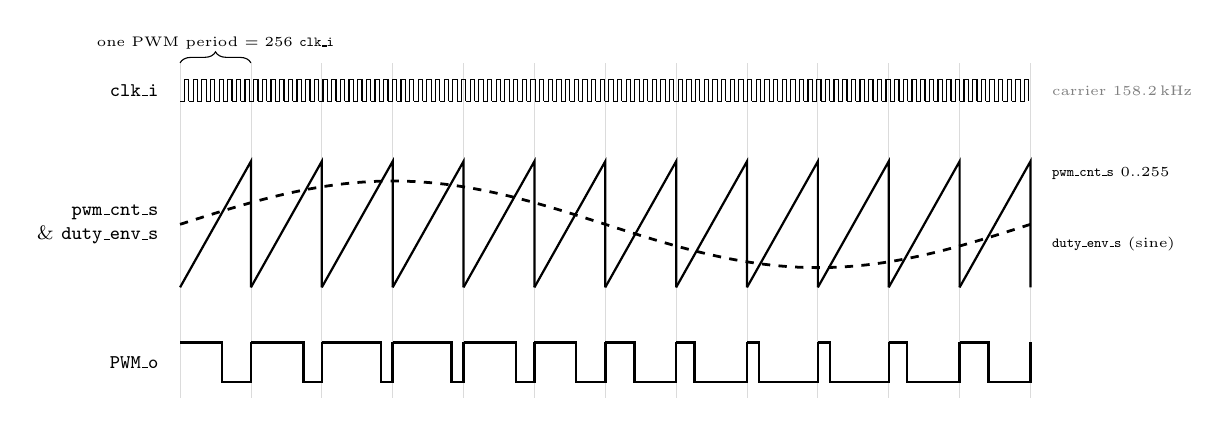
\begin{tikzpicture}[every node/.style={font=\scriptsize}]
\def\N{12}\def\W{0.9}\def\xo{1.2}
\def\yclk{2.5}\def\ybot{0.0}\def\ytop{1.6}
\def\yhi{-0.7}\def\ylo{-1.2}
\node[anchor=east] at (\xo-0.15,\yclk){\texttt{clk\_i}};
\node[anchor=east, align=right] at (\xo-0.15,0.8){\texttt{pwm\_cnt\_s}\\[1pt] \& \texttt{duty\_env\_s}};
\node[anchor=east] at (\xo-0.15,{(\yhi+\ylo)/2}){\texttt{PWM\_o}};
% vertical grid separating the PWM periods
\foreach \i in {0,...,12}{
  \draw[black!14, line width=0.3pt] ({\xo+\i*\W},{\ylo-0.2}) -- ({\xo+\i*\W},{\yclk+0.35});}
% clk_i continuous (schematic, much faster)
\clkspan{\xo}{\xo+\N*\W}{\yclk}{0.11}
\draw[decorate,decoration={brace,amplitude=4pt},line width=0.4pt] (\xo,{\yclk+0.35}) -- ({\xo+\W},{\yclk+0.35});
\node[anchor=south,font=\tiny] at ({\xo+0.5*\W},{\yclk+0.4}){one PWM period $=256$ \texttt{clk\_i}};
\node[anchor=west,font=\tiny,gray] at ({\xo+\N*\W+0.15},\yclk){carrier $158.2$\,kHz};
% sawtooth carrier pwm_cnt_s
\foreach \i in {0,...,11}{
  \draw[line width=0.8pt] ({\xo+\i*\W},\ybot) -- ({\xo+(\i+1)*\W},\ytop) -- ({\xo+(\i+1)*\W},\ybot);}
\node[anchor=west,font=\tiny] at ({\xo+\N*\W+0.15},{\ytop-0.15}){\texttt{pwm\_cnt\_s} 0..255};
% sine modulator duty_env_s
\draw[line width=1.0pt, dashed, smooth, samples=120, domain=0:10.8]
  plot ({\xo+\x},{0.8+0.55*sin(\x/10.8*360)});
\node[anchor=west,font=\tiny] at ({\xo+\N*\W+0.15},0.55){\texttt{duty\_env\_s} (sine)};
% PWM_o: high while pwm_cnt_s < duty_env_s
\foreach \i in {0,...,11}{
  \pgfmathsetmacro\sv{0.8+0.55*sin((\i+0.5)/12*360)}
  \pgfmathsetmacro\wid{(\sv/1.6)*\W}
  \draw[line width=0.9pt]
    ({\xo+\i*\W},\yhi) -- ({\xo+\i*\W+\wid},\yhi) -- ({\xo+\i*\W+\wid},\ylo)
    -- ({\xo+(\i+1)*\W},\ylo) -- ({\xo+(\i+1)*\W},\yhi);}
\end{tikzpicture}}
\caption{Sinusoidal PWM: \texttt{pwm\_cnt\_s} ramps 0 to 255 each period and \texttt{PWM\_o}
is high while it is below \texttt{duty\_env\_s}, so the pulse width traces the sine
(\texttt{pwm\_generic\_master.vhd}).}
\label{fig:spwm}
\end{figure}

% =====================================================================
\section{Display}
\label{sec:display}
% =====================================================================

The display uses \texttt{spi\_display.vhd}, a transmit only SPI in mode 3 (SCK idles high,
the panel reads each bit on the rising edge). The clock uses a $\div6$ prescaler, so the
SCK is $40.5\,\mathrm{MHz}/6 = 6.75$\,MHz. In clock cycles, one SCK is 6 \texttt{clk\_i} and
one byte is $8\times6 = 48$ \texttt{clk\_i} $= 1.19\,\mu$s. DC, RST and CS are register
bits; the FSM has three states (Figure~\ref{fig:disp-fsm}), and after the eighth bit SCK
parks high, which is the mode 3 idle, so byte boundaries need no extra states.

On top of the SPI, the firmware draws a small dashboard on the panel. At boot it first
sends the ST7789 init sequence (SWRESET, SLPOUT, COLMOD RGB565, MADCTL landscape, INVON,
NORON, DISPON), each command with its datasheet delay. After that the drawing works step by
step. When the firmware wants to draw something it does not send it right away: it puts the
drawing as a small job in a queue that holds up to 48 jobs. Then, once per main loop, the
function \texttt{display\_tick()} takes one job from the queue and sends only a small chunk
of SPI bytes (128 to 384 bytes, about 150 to $450\,\mu$s). This chunk is short next to the
10.9\,ms frame, so it does not slow down the tone player. If instead the firmware drew a
full screen in one go, the SPI would take about 180\,ms and block the main loop, which would
stop the tone and fill up the command FIFO. Sending small chunks avoids this.

Four fixed zones show slave health, the live spectrum
(bins 16 to 55 straight from the snapshot), RX/TX symbols and a log ring; which
content each zone shows and the three theme colours come from the NOR settings, so
the web dashboard restyles the display remotely.

\begin{figure}[H]
\centering
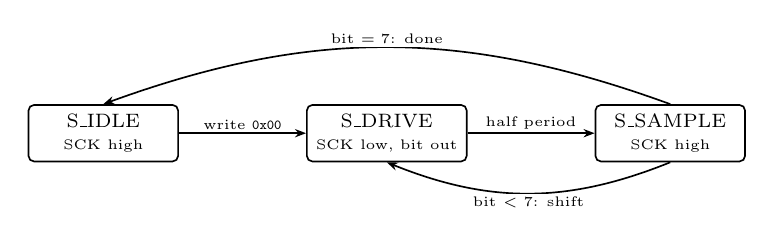
\begin{tikzpicture}[
    every node/.style={font=\scriptsize},
    st/.style={rounded corners=2pt, draw, line width=0.6pt, fill=white, minimum width=1.9cm, minimum height=0.7cm, align=center},
    a/.style={-{Stealth[length=4pt]}, line width=0.6pt},
    al/.style={font=\tiny, fill=white, inner sep=1pt}
]
\node[st] (idle) at (0,0)   {S\_IDLE\\ \tiny SCK high};
\node[st] (lo)   at (3.6,0) {S\_DRIVE\\ \tiny SCK low, bit out};
\node[st] (hi)   at (7.2,0) {S\_SAMPLE\\ \tiny SCK high};
\draw[a] (idle) -- node[al,above]{write \texttt{0x00}} (lo);
\draw[a] (lo) -- node[al,above]{half period} (hi);
\draw[a] (hi.south) to[bend left=22] node[al,below]{bit $<7$: shift} (lo.south);
\draw[a] (hi.north) to[bend right=20] node[al,above]{bit $=7$: done} (idle.north);
\end{tikzpicture}
\caption{Display SPI FSM (\texttt{spi\_display.vhd}).}
\label{fig:disp-fsm}
\end{figure}

\begin{figure}[H]
\centering
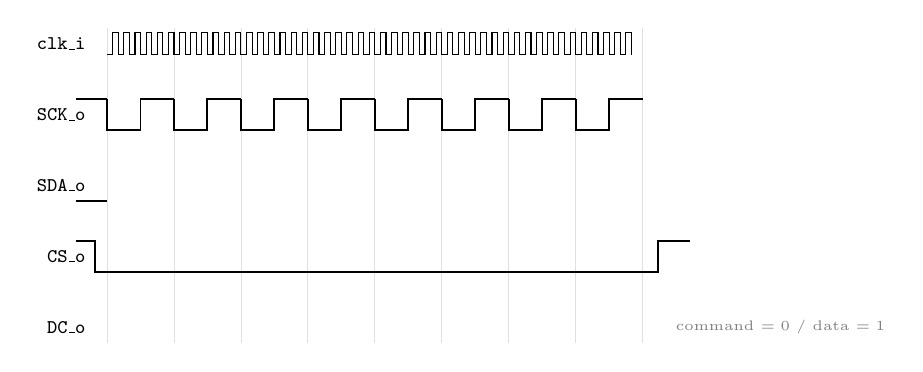
\begin{tikzpicture}[every node/.style={font=\scriptsize}]
\def\yclk{0}\def\yck{-0.9}\def\ysda{-1.8}\def\ycs{-2.7}\def\ydc{-3.6}
\def\bw{0.85}\def\xo{1.0}
\node[anchor=east] at (0.85,\yclk){\texttt{clk\_i}};
\node[anchor=east] at (0.85,\yck){\texttt{SCK\_o}};
\node[anchor=east] at (0.85,\ysda){\texttt{SDA\_o}};
\node[anchor=east] at (0.85,\ycs){\texttt{CS\_o}};
\node[anchor=east] at (0.85,\ydc){\texttt{DC\_o}};
\sgrid{\xo}{8}{\bw}{0.2}{-3.8}
\clkspan{\xo}{\xo+8*\bw}{\yclk}{0.1417}
\draw[line width=0.7pt] ({\xo-0.4},\yck+0.2) -- (\xo,\yck+0.2);
\foreach \i in {0,...,7}{
  \draw[line width=0.7pt]
   ({\xo+\i*\bw},\yck+0.2) -- ({\xo+\i*\bw},\yck-0.2)
   -- ({\xo+\i*\bw+0.5*\bw},\yck-0.2) -- ({\xo+\i*\bw+0.5*\bw},\yck+0.2)
   -- ({\xo+(\i+1)*\bw},\yck+0.2);}
\foreach \i/\b in {0/b7,1/b6,2/b5,3/b4,4/b3,5/b2,6/b1,7/b0}{
  \pbus{\xo+\i*\bw}{\xo+(\i+1)*\bw}{\ysda}{\b}}
\draw[line width=0.7pt] ({\xo-0.4},\ysda-0.2) -- (\xo,\ysda-0.2);
\draw[line width=0.7pt] ({\xo-0.4},\ycs+0.2) -- ({\xo-0.15},\ycs+0.2) -- ({\xo-0.15},\ycs-0.2)
  -- ({\xo+8*\bw+0.2},\ycs-0.2) -- ({\xo+8*\bw+0.2},\ycs+0.2) -- ({\xo+8*\bw+0.6},\ycs+0.2);
\plow{\xo-0.4}{\xo+8*\bw+0.6}{\ydc}
\node[anchor=west,font=\tiny,gray] at ({\xo+8*\bw+0.3},\ydc){command $=0$ / data $=1$};
\end{tikzpicture}
\caption{One display byte (\texttt{spi\_display.vhd}).}
\label{fig:disp-wave}
\end{figure}

% =====================================================================
\section{NOR flash storage}
\label{sec:flash}
% =====================================================================

The CPU manages NOR storage in firmware (\texttt{norflash.c}). The ESP32 sends one
character opcodes on the S7 UART (pins 72/20), and \texttt{nor\_poll()}, a non blocking
step in the main loop, reads each opcode and runs the matching W25Q64 SPI sequence; the
SPI frames go out through the generic S8 master at 633\,kHz. At power up
\texttt{nor\_init()} runs the boot chain, then the loop sits in the IDLE hub and
dispatches each opcode with a \texttt{case} (Figure~\ref{fig:flash-fsm}).

The chip uses the standard W25Q64 opcodes (Table~\ref{tab:nor-cmd}). Every access is one
SPI transaction: CS goes low, the master (\texttt{spi\_master\_generic.vhd}) clocks the
command byte MSB first, then a 24 bit address if the command needs one, then data, and CS
goes high. A read (\texttt{0x03}) sends the address and the chip drives the bytes back on
MISO (Figure~\ref{fig:nor-read}). A write is longer: a Write Enable (\texttt{0x06}) frame
first, then a Page Program (\texttt{0x02}) with the address and the data, then the master
polls the status register (\texttt{0x05}) until the WIP bit is 0
(Figure~\ref{fig:nor-write}). An erase works like the program, with \texttt{0x20} and no
data.

In clock cycles: SCK is \texttt{clk\_i}$/64 = 633$\,kHz, so one SCK is 64 clocks and one
byte is $8\times64 = 512$ clocks ($12.6\,\mu$s). A read is the command byte plus the 3
address bytes ($4\times512 = 2048$ clocks $= 50.6\,\mu$s) and then one more byte per data
byte read. A page program is the WREN byte, then the command, 3 address bytes and up to
256 data bytes, so 260 SPI bytes; after that the status poll runs until the WIP bit
clears, and that wait is set by the chip's internal program time, not by SPI clocks.

\begin{table}[H]
\centering
\caption{W25Q64 SPI commands used.}
\label{tab:nor-cmd}
\begin{tabular}{lll}
\hline
Code & Name & Use \\
\hline
\texttt{0x06} & Write Enable & set before every program or erase \\
\texttt{0x01} & Write Status Register & set QE, clear the protection bits \\
\texttt{0x98} & Global Block Unlock & clear all block protection \\
\texttt{0x05} & Read Status Register & polled for the WIP (busy) bit \\
\texttt{0x9F} & JEDEC ID & read manufacturer and device id \\
\texttt{0x03} & Read Data & read bytes from a 24 bit address \\
\texttt{0x02} & Page Program & write up to 256 bytes at a 24 bit address \\
\texttt{0x20} & Sector Erase & erase one 4\,KB sector \\
\hline
\end{tabular}
\end{table}

\begin{figure}[H]
\centering
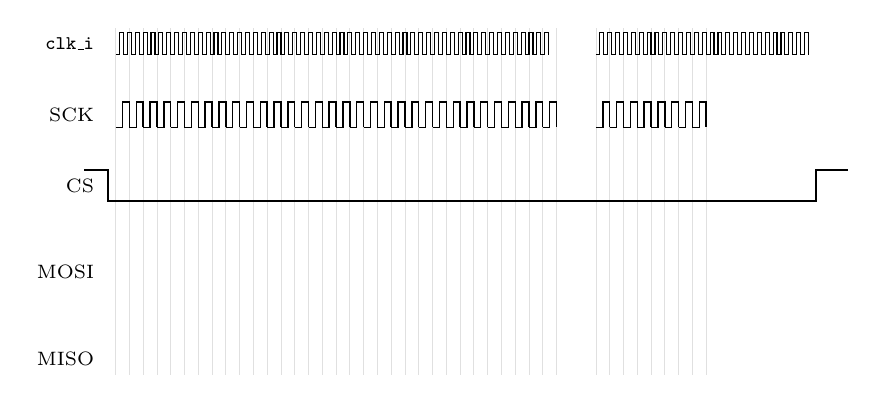
\begin{tikzpicture}[every node/.style={font=\scriptsize}]
\def\yclk{0}\def\ysck{-0.9}\def\ycs{-1.8}\def\ymo{-2.9}\def\ymi{-4.0}
\def\bw{1.4}\def\xo{1.0}
\node[anchor=east] at (0.85,\yclk){\texttt{clk\_i}};
\node[anchor=east] at (0.85,\ysck){SCK};
\node[anchor=east] at (0.85,\ycs){CS};
\node[anchor=east] at (0.85,\ymo){MOSI};
\node[anchor=east] at (0.85,\ymi){MISO};
\sgrid{\xo}{32}{\bw/8}{0.2}{-4.2}
\sgrid{\xo+4*\bw+0.5}{8}{\bw/8}{0.2}{-4.2}
\clkspan{\xo}{\xo+4*\bw}{\yclk}{0.1}
\pcut{\xo+4*\bw+0.15}{\yclk-0.16}{\yclk+0.16}
\clkspan{\xo+4*\bw+0.5}{\xo+6*\bw+0.5}{\yclk}{0.1}
\foreach \k in {0,1,2,3}{\sckbyte{\xo+\k*\bw}{\ysck}{\bw}}
\pcut{\xo+4*\bw+0.15}{\ysck-0.2}{\ysck+0.2}
\sckbyte{\xo+4*\bw+0.5}{\ysck}{\bw}
\draw[line width=0.7pt] ({\xo-0.4},\ycs+0.2)--({\xo-0.1},\ycs+0.2)--({\xo-0.1},\ycs-0.2)
  --({\xo+6*\bw+0.5},\ycs-0.2)--({\xo+6*\bw+0.5},\ycs+0.2)--({\xo+6*\bw+0.9},\ycs+0.2);
\pbus{\xo}{\xo+\bw}{\ymo}{\texttt{0x03}}
\pbus{\xo+\bw}{\xo+2*\bw}{\ymo}{A[23:16]}
\pbus{\xo+2*\bw}{\xo+3*\bw}{\ymo}{A[15:8]}
\pbus{\xo+3*\bw}{\xo+4*\bw}{\ymo}{A[7:0]}
\pcut{\xo+4*\bw+0.15}{\ymo-0.2}{\ymo+0.2}
\pbus{\xo+4*\bw+0.5}{\xo+5*\bw+0.5}{\ymo}{--}
\plow{\xo-0.4}{\xo+4*\bw}{\ymi}
\pcut{\xo+4*\bw+0.15}{\ymi-0.2}{\ymi+0.2}
\pbus{\xo+4*\bw+0.5}{\xo+5*\bw+0.5}{\ymi}{D0}
\pbus{\xo+5*\bw+0.5}{\xo+6*\bw+0.5}{\ymi}{D1}
\end{tikzpicture}
\caption{NOR flash read \texttt{0x03} (\texttt{spi\_master\_generic.vhd}, S8 to W25Q64).}
\label{fig:nor-read}
\end{figure}

\begin{figure}[H]
\centering
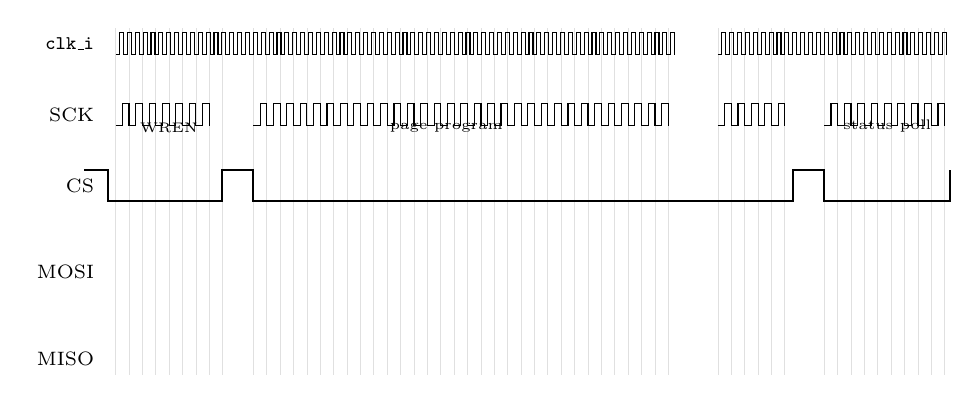
\begin{tikzpicture}[every node/.style={font=\scriptsize}]
\def\yclk{0}\def\ysck{-0.9}\def\ycs{-1.8}\def\ymo{-2.9}\def\ymi{-4.0}
\def\bw{1.35}\def\xo{1.0}
\node[anchor=east] at (0.85,\yclk){\texttt{clk\_i}};
\node[anchor=east] at (0.85,\ysck){SCK};
\node[anchor=east] at (0.85,\ycs){CS};
\node[anchor=east] at (0.85,\ymo){MOSI};
\node[anchor=east] at (0.85,\ymi){MISO};
\sgrid{1.0}{8}{0.17}{0.2}{-4.2}
\sgrid{2.75}{31}{0.17}{0.2}{-4.2}
\sgrid{8.65}{5}{0.17}{0.2}{-4.2}
\sgrid{10.0}{9}{0.17}{0.2}{-4.2}
\clkspan{1.0}{8.15}{\yclk}{0.1}
\pcut{8.3}{\yclk-0.16}{\yclk+0.16}
\clkspan{8.65}{11.6}{\yclk}{0.1}
\clkspan{1.0}{2.35}{\ysck}{0.17}
\clkspan{2.75}{8.15}{\ysck}{0.17}
\pcut{8.3}{\ysck-0.2}{\ysck+0.2}
\clkspan{8.65}{9.6}{\ysck}{0.17}
\clkspan{10.0}{11.6}{\ysck}{0.17}
\draw[line width=0.7pt] ({\xo-0.4},\ycs+0.2)--({\xo-0.1},\ycs+0.2)--({\xo-0.1},\ycs-0.2)
  --({\xo+\bw},\ycs-0.2)--({\xo+\bw},\ycs+0.2)
  --({\xo+\bw+0.4},\ycs+0.2)--({\xo+\bw+0.4},\ycs-0.2)
  --(9.6,\ycs-0.2)--(9.6,\ycs+0.2)
  --(10.0,\ycs+0.2)--(10.0,\ycs-0.2)
  --(11.6,\ycs-0.2)--(11.6,\ycs+0.2);
\node[anchor=south,font=\tiny] at ({\xo+0.5*\bw},\ycs+0.55){WREN};
\node[anchor=south,font=\tiny] at (5.2,\ycs+0.55){page program};
\node[anchor=south,font=\tiny] at (10.8,\ycs+0.55){status poll};
\pbus{\xo}{\xo+\bw}{\ymo}{\texttt{0x06}}
\pbus{\xo+\bw+0.4}{\xo+2*\bw+0.4}{\ymo}{\texttt{0x02}}
\pbus{\xo+2*\bw+0.4}{\xo+3*\bw+0.4}{\ymo}{A[23:16]}
\pbus{\xo+3*\bw+0.4}{\xo+4*\bw+0.4}{\ymo}{A[15:8]}
\pbus{\xo+4*\bw+0.4}{\xo+5*\bw+0.4}{\ymo}{A[7:0]}
\pcut{8.3}{\ymo-0.2}{\ymo+0.2}
\pbus{8.65}{9.6}{\ymo}{data}
\pbus{10.0}{10.8}{\ymo}{\texttt{0x05}}
\pbus{10.8}{11.6}{\ymo}{--}
\plow{\xo-0.4}{10.8}{\ymi}
\pbus{10.8}{11.6}{\ymi}{status}
\end{tikzpicture}
\caption{NOR flash page program \texttt{0x02} with Write Enable and status poll
(\texttt{spi\_master\_generic.vhd}).}
\label{fig:nor-write}
\end{figure}

\textbf{Memory layout.} The first 12\,KB: sector 0 (4\,KB) holds a 32 byte settings
blob (magic \texttt{0xA5}, device name, auto presence interval, retry count, debug
flag, display theme colours, view flags, v2 marker \texttt{0x5A}); sectors 1 to 2 hold the
log, 512 slots of 16 bytes (sequence, type character, timestamp, value, 8 ASCII
bytes) managed as a ring buffer. At power up a SCAN reads the type byte of all 512
slots and takes head $=$ (highest valid $+1$) mod 512; treating anything outside the
valid type set as empty makes the scan robust to the holes an aborted write leaves.

\textbf{Unlock before the id read.} On this board \texttt{/HOLD} and \texttt{/WP} float,
and a floating \texttt{/HOLD} picks up SCK edges, so the chip pauses mid frame and every
read returns \texttt{0xFF}, including the JEDEC id. Reading the id first is therefore not
reliable: the first frames at boot are a WRSR that sets QE$=1$ (which frees those pins)
and clears the protection bits, then a Global Block Unlock, and only then the id read for
the presence flag. A wrong id makes every later opcode fail fast instead of waiting for
timeouts. The timeouts count time, not loop iterations: 2\,ms per SPI byte, 700\,ms on
the WIP poll (a sector erase can take 400\,ms), and 200\,ms per payload byte from the
ESP32.

\begin{figure}[H]
\centering
\resizebox{0.94\textwidth}{!}{%
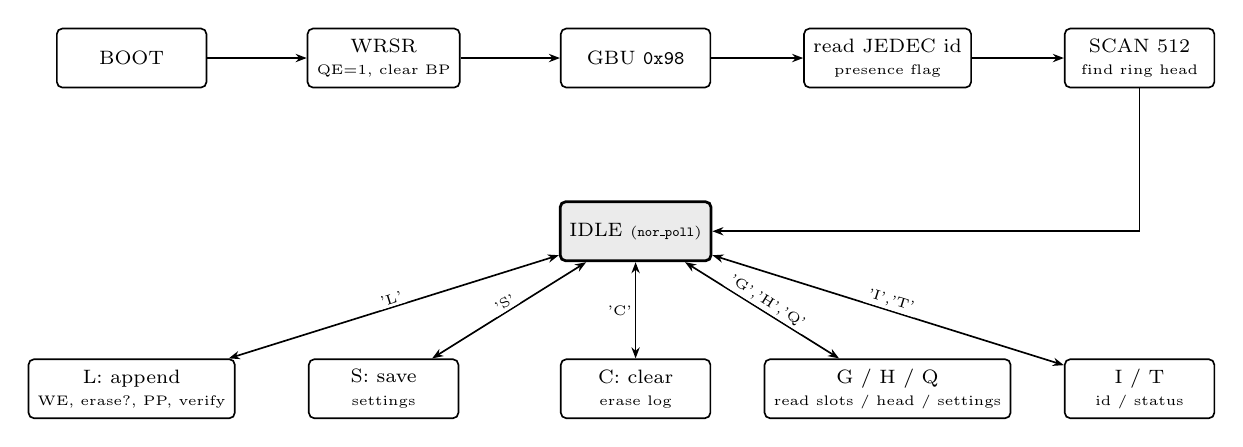
\begin{tikzpicture}[
    every node/.style={font=\footnotesize},
    st/.style={rounded corners=2pt, draw, line width=0.6pt, fill=white, minimum width=1.9cm, minimum height=0.75cm, align=center, font=\scriptsize},
    acc/.style={rounded corners=2pt, draw, line width=1.0pt, fill=black!8, minimum width=1.9cm, minimum height=0.75cm, align=center, font=\scriptsize},
    a/.style={-{Stealth[length=4pt]}, line width=0.6pt},
    b/.style={{Stealth[length=4pt]}-{Stealth[length=4pt]}, line width=0.6pt},
    al/.style={font=\tiny, fill=white, inner sep=1pt}
]
\node[st] (boot) at (0,0)    {BOOT};
\node[st] (wrsr) at (3.2,0)  {WRSR\\ \tiny QE$=$1, clear BP};
\node[st] (gbu)  at (6.4,0)  {GBU \texttt{0x98}};
\node[st] (rd)   at (9.6,0)  {read JEDEC id\\ \tiny presence flag};
\node[st] (scan) at (12.8,0) {SCAN 512\\ \tiny find ring head};
\draw[a] (boot)--(wrsr); \draw[a] (wrsr)--(gbu); \draw[a] (gbu)--(rd); \draw[a] (rd)--(scan);
\node[acc] (idle) at (6.4,-2.2) {IDLE \tiny (\texttt{nor\_poll})};
\draw[a] (scan) |- (idle);
\node[st] (ap) at (0,-4.2)    {L: append\\ \tiny WE, erase?, PP, verify};
\node[st] (sw) at (3.2,-4.2)  {S: save\\ \tiny settings};
\node[st] (cl) at (6.4,-4.2)  {C: clear\\ \tiny erase log};
\node[st] (g)  at (9.6,-4.2)  {G / H / Q\\ \tiny read slots / head / settings};
\node[st] (t)  at (12.8,-4.2) {I / T\\ \tiny id / status};
\draw[b] (idle)-- node[al,sloped,above]{'L'}(ap);
\draw[b] (idle)-- node[al,sloped,above]{'S'}(sw);
\draw[b] (idle)-- node[al,left]{'C'}(cl);
\draw[b] (idle)-- node[al,sloped,above]{'G','H','Q'}(g);
\draw[b] (idle)-- node[al,sloped,above]{'I','T'}(t);
\end{tikzpicture}%
}
\caption{Storage FSM (\texttt{norflash.c}).}
\label{fig:flash-fsm}
\end{figure}

\textbf{Board notes.} A few problems only appeared on the wiring, not in simulation. A
4\,KB sector erase draws about $80$\,mA for up to 400\,ms from an internal charge pump;
with no local decoupling the 3.3\,V rail dropped at the chip ($\Delta V = I\,t/C$) and it
browned out mid erase, dropping the program that followed. A 1\,$\mu$F ceramic alone still
gave $\Delta V = 0.08\cdot0.03/10^{-6} = 2.4$\,V of droop, so 1\,$\mu$F and 10\,$\mu$F in
parallel bring it to $0.22$\,V and keep the rail above the 2.7\,V minimum (the two values
cover the fast edges and the slow pump). 5\,MHz SPI was also too fast for the jumpers and
long writes arrived truncated; at 633\,kHz ($\div64$, bit time $1.58\,\mu$s) writes became
reliable ($95$\,\% for records, $85$\,\% for settings saves), and the firmware adds up to
5 retries with read back, so the effective loss is zero and a failed attempt only burns a
ring slot that the SCAN later skips. One more note: an LED without a series resistor
injected current into the shared ground and disturbed the ADC, UART and SPI at once, so
LEDs on logic pins always get a 330\,$\Omega$ to 1\,k$\Omega$ resistor.

% =====================================================================
\section{The UART links}
\label{sec:uart}
% =====================================================================

The FPGA has two identical UARTs from \texttt{uart\_generic.vhd}: the character UART (S6,
pins 17/18) that carries diagnostics and banner text, and the NOR command UART (S7, pins
72/20) that carries the one character flash opcodes. They are two instances of the same
block with the same register map (Table~\ref{tab:addrmap}): \texttt{0x00} writes a byte to
send and reads the received byte (bit 8 is the valid flag), \texttt{0x04} and \texttt{0x08}
enable and disable, \texttt{0x0C} sets the baud divider and \texttt{0x10} the format, and
\texttt{0x14} is the status (\texttt{rx\_valid}, \texttt{tx\_busy}). At 115\,200 baud the
divider is 352, so one bit lasts 352 clocks.

Each instance has a transmit and a receive state machine (Figure~\ref{fig:uart-fsm}). On
transmit, a write to \texttt{0x00} sets \texttt{tx\_busy} and the machine sends a start
bit, 8 data bits LSB first, an optional parity bit and a stop bit
(Figure~\ref{fig:uart-wave}). On receive, two flip flops (\texttt{rx\_q0},
\texttt{rx\_q1}) synchronise the line; a falling edge starts the machine, it samples the
first bit at half a bit time and the rest one bit time apart, and each finished byte goes
into a 16 deep FIFO (\texttt{rxf}) that the master reads from \texttt{0x00}.

\begin{figure}[H]
\centering
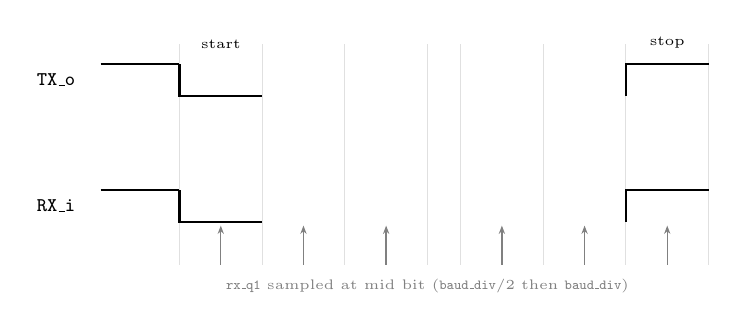
\begin{tikzpicture}[every node/.style={font=\scriptsize}]
\def\ytx{0}\def\yrx{-1.6}
\def\bw{1.05}\def\xo{1.2}
\node[anchor=east] at (0.0,\ytx){\texttt{TX\_o}};
\node[anchor=east] at (0.0,\yrx){\texttt{RX\_i}};
% vertical grid tied to the bit period
\sgrid{\xo}{3}{\bw}{0.45}{-2.35}
\sgrid{\xo+3.4*\bw}{3}{\bw}{0.45}{-2.35}
\draw[line width=0.8pt] (0.2,\ytx+0.2)--(\xo,\ytx+0.2);
\draw[line width=0.8pt] (\xo,\ytx+0.2)--(\xo,\ytx-0.2)--({\xo+\bw},\ytx-0.2);
\pbus{\xo+\bw}{\xo+2*\bw}{\ytx}{D0}\pbus{\xo+2*\bw}{\xo+3*\bw}{\ytx}{D1}
\pcut{\xo+3*\bw+0.15}{\ytx-0.2}{\ytx+0.2}
\pbus{\xo+3.4*\bw}{\xo+4.4*\bw}{\ytx}{D6}\pbus{\xo+4.4*\bw}{\xo+5.4*\bw}{\ytx}{D7}
\draw[line width=0.8pt] ({\xo+5.4*\bw},\ytx-0.2)--({\xo+5.4*\bw},\ytx+0.2)--({\xo+6.4*\bw},\ytx+0.2);
\node[anchor=south,font=\tiny] at ({\xo+0.5*\bw},\ytx+0.28){start};
\node[anchor=south,font=\tiny] at ({\xo+5.9*\bw},\ytx+0.28){stop};
\draw[line width=0.8pt] (0.2,\yrx+0.2)--(\xo,\yrx+0.2);
\draw[line width=0.8pt] (\xo,\yrx+0.2)--(\xo,\yrx-0.2)--({\xo+\bw},\yrx-0.2);
\pbus{\xo+\bw}{\xo+2*\bw}{\yrx}{D0}\pbus{\xo+2*\bw}{\xo+3*\bw}{\yrx}{D1}
\pcut{\xo+3*\bw+0.15}{\yrx-0.2}{\yrx+0.2}
\pbus{\xo+3.4*\bw}{\xo+4.4*\bw}{\yrx}{D6}\pbus{\xo+4.4*\bw}{\xo+5.4*\bw}{\yrx}{D7}
\draw[line width=0.8pt] ({\xo+5.4*\bw},\yrx-0.2)--({\xo+5.4*\bw},\yrx+0.2)--({\xo+6.4*\bw},\yrx+0.2);
\foreach \k in {0.5,1.5,2.5,3.9,4.9,5.9}{
  \draw[-{Stealth[length=3pt]},line width=0.5pt,gray] ({\xo+\k*\bw},\yrx-0.75)--({\xo+\k*\bw},\yrx-0.25);}
\node[anchor=north,font=\tiny,gray] at ({\xo+3*\bw},\yrx-0.8){\texttt{rx\_q1} sampled at mid bit (\texttt{baud\_div}/2 then \texttt{baud\_div})};
\end{tikzpicture}
\caption{UART frame, 8N1 (\texttt{uart\_generic.vhd}). One bit is \texttt{baud\_div}
clocks; data goes LSB first.}
\label{fig:uart-wave}
\end{figure}

\begin{figure}[H]
\centering
\resizebox{0.96\textwidth}{!}{%
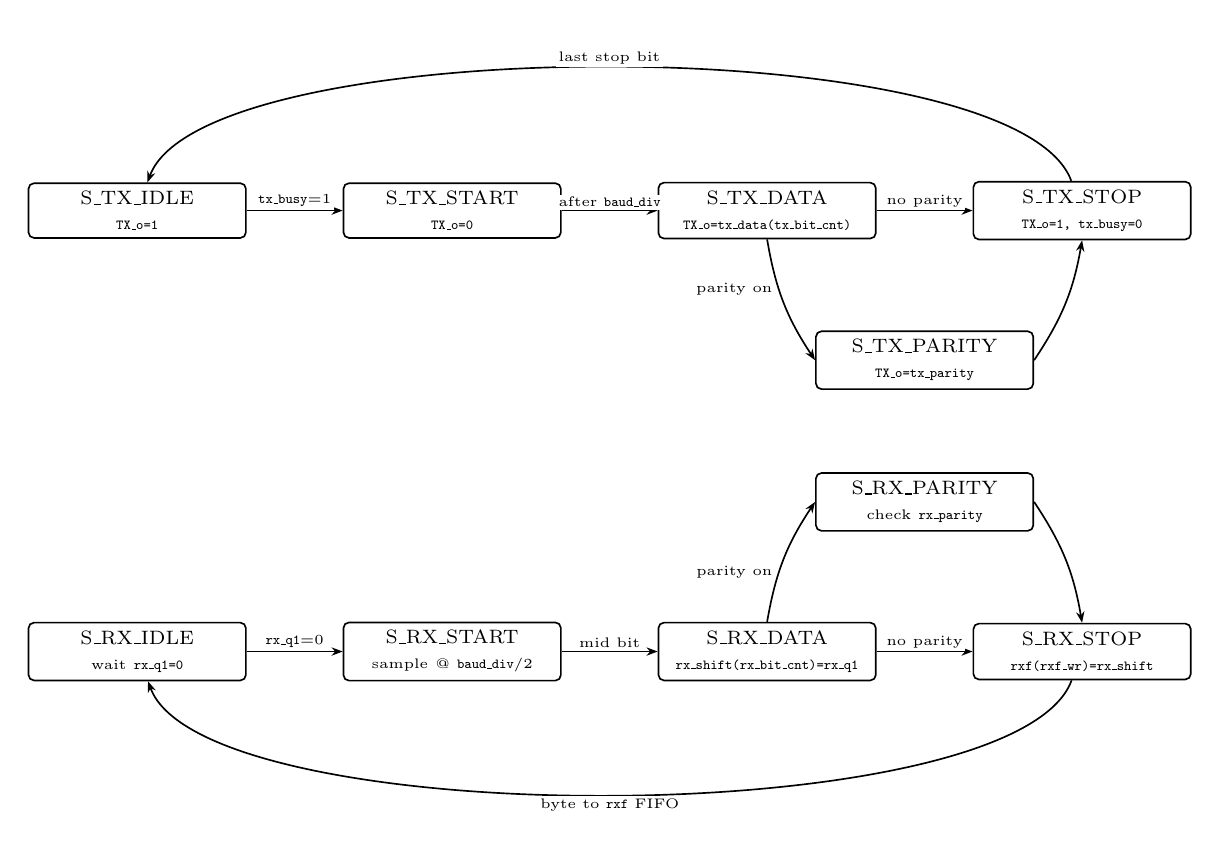
\begin{tikzpicture}[
  every node/.style={font=\scriptsize},
  st/.style={rounded corners=2pt, draw, line width=0.6pt, fill=white, text width=2.55cm, align=center, inner sep=3pt},
  a/.style={-{Stealth[length=4pt]}, line width=0.6pt},
  al/.style={font=\tiny, fill=white, inner sep=1pt}]
\node[st] (ti) at (0,0)    {S\_TX\_IDLE\\[1pt] \tiny \texttt{TX\_o=1}};
\node[st] (ts) at (4.0,0)  {S\_TX\_START\\[1pt] \tiny \texttt{TX\_o=0}};
\node[st] (td) at (8.0,0)  {S\_TX\_DATA\\[1pt] \tiny \texttt{TX\_o=tx\_data(tx\_bit\_cnt)}};
\node[st] (to) at (12.0,0) {S\_TX\_STOP\\[1pt] \tiny \texttt{TX\_o=1, tx\_busy=0}};
\node[st] (tp) at (10.0,-1.9) {S\_TX\_PARITY\\[1pt] \tiny \texttt{TX\_o=tx\_parity}};
\draw[a] (ti)-- node[al,above]{\texttt{tx\_busy}=1}(ts);
\draw[a] (ts)-- node[al,above]{after \texttt{baud\_div}}(td);
\draw[a] (td)-- node[al,above]{no parity}(to);
\draw[a] (td.south) to[bend right=12] node[al,below left,pos=0.3]{parity on}(tp.west);
\draw[a] (tp.east) to[bend right=12] (to.south);
\draw[a] (to) to[out=110,in=70,looseness=0.45] node[al,above]{last stop bit}(ti);
\node[st] (ri) at (0,-5.6)    {S\_RX\_IDLE\\[1pt] \tiny wait \texttt{rx\_q1=0}};
\node[st] (rs) at (4.0,-5.6)  {S\_RX\_START\\[1pt] \tiny sample @ \texttt{baud\_div}/2};
\node[st] (rd) at (8.0,-5.6)  {S\_RX\_DATA\\[1pt] \tiny \texttt{rx\_shift(rx\_bit\_cnt)=rx\_q1}};
\node[st] (ro) at (12.0,-5.6) {S\_RX\_STOP\\[1pt] \tiny \texttt{rxf(rxf\_wr)=rx\_shift}};
\node[st] (rp) at (10.0,-3.7) {S\_RX\_PARITY\\[1pt] \tiny check \texttt{rx\_parity}};
\draw[a] (ri)-- node[al,above]{\texttt{rx\_q1}=0}(rs);
\draw[a] (rs)-- node[al,above]{mid bit}(rd);
\draw[a] (rd)-- node[al,above]{no parity}(ro);
\draw[a] (rd.north) to[bend left=12] node[al,above left,pos=0.3]{parity on}(rp.west);
\draw[a] (rp.east) to[bend left=12] (ro.north);
\draw[a] (ro) to[out=250,in=290,looseness=0.45] node[al,below]{byte to \texttt{rxf} FIFO}(ri);
\end{tikzpicture}}
\caption{UART transmit and receive state machines (\texttt{uart\_generic.vhd}).}
\label{fig:uart-fsm}
\end{figure}

% =====================================================================
\section{Firmware}
\label{sec:firmware}
% =====================================================================

The PicoRV32 firmware is seven C files plus a startup, compiled for
\texttt{rv32imc}, code in the 32\,KB ITCM, data in the 16\,KB DTCM (both CPU local,
off the bus); the build flattens the binary into the word per line hex file the IP
wants as ITCM initialisation, so the firmware travels inside the bitstream. The
structure is a single main loop, no OS and deliberately no interrupts
(Section~\ref{sec:fetch}); every call is non blocking: \texttt{emit\_capture} queues
protocol characters received from the ESP32; \texttt{emit\_player\_tick} pops one
and plays it (write tone pair to the PWM, 144\,ms on, stop, 400\,ms silence), and
also enforces carrier sense, while the slave carrier has been heard in the last
3\,s the player holds the queue, and if the carrier appears mid tone it stops the
PWM at once; \texttt{decode\_step} polls \texttt{fill\_cnt}, copies the snapshot on
a change and decodes it, forwarding to the ESP32 only the uppercase symbols riding
the slave carrier (lowercase ones are the master hearing itself, kept as a loopback
check); \texttt{nor\_poll} runs the storage protocol; \texttt{display\_tick} pushes
one display chunk. Every 15\,s \texttt{health\_tick} reads one safe register from each
slave, sanity checks the value, ORs the result with the previous scan (one dirty
read cannot flag a healthy slave) and emits a \texttt{\$HLT} mask that both the
dashboard and the display render; at boot it prints a probe marker before each first
touch, so if a slave hangs the CPU the last marker names the culprit, that trick
found the GPIO ack bug in minutes. Diagnostics share the character UART framed as
\texttt{\$...}$\backslash$\texttt{n} lines that the ESP32 forwards to the USB
console instead of the protocol parser, gated by a debug flag stored in the NOR
settings and toggled live from the dashboard.

The ESP32 side is small modules: a register level UART driver (FIFO, CLKDIV,
CONF0/STATUS registers directly; 115200 from the 80\,MHz APB is CLKDIV
$694+7/16$, $0.007$\,\% off), \texttt{flash\_link} with retry and read back
verification plus a RAM cache for the dashboard, the codebook layer, the protocol
state machine, and the WebSocket/JSON client, which also caps Wi-Fi transmit power
at 11\,dBm after full power bursts tripped the brownout detector on a weak supply.

% =====================================================================
\section{The acoustic protocol}
\label{sec:protocol}
% =====================================================================

The protocol uses an \emph{alternating bit codebook}. A pattern is two or three
symbols in which two consecutive symbols must differ, so the receiver triggers on a
\emph{change} of tone, easy to see, rather than on silence, which is hard to
measure on a noisy channel. Six symbols exist: lowercase \texttt{a,b,c} (bit 0,
bit 1, EOF) ride the 2014\,Hz master carrier (FFT bin 22), uppercase
\texttt{A,B,C} ride the 2472\,Hz slave carrier (bin 27); EOF, bit 0 and bit 1 use
2930, 3571 and 4577\,Hz (bins 32, 39, 50), all exact bin centres of the shared
$91.6$\,Hz grid, the closest pair 7 bins apart. A message is identified by its first
bit and length, the carrier gives the direction (Table~\ref{tab:codebook}); every
pattern is framed by EOF at both ends.

\begin{table}[H]
\centering
\caption{The codebook.}
\label{tab:codebook}
\small
\begin{tabular}{llll}
\toprule
\textbf{Pattern} & \textbf{(first, len)} & \textbf{Master carrier (to slave)} & \textbf{Slave carrier (to master)} \\
\midrule
\texttt{01} & (0, 2) & presence request & presence: yes \\
\texttt{10} & (1, 2) & assign id ($=1$) & presence: no \\
\texttt{010} & (0, 3) & abort & registration request \\
\texttt{101} & (1, 3) &, & acknowledge \\
\bottomrule
\end{tabular}
\end{table}

On the air each transmission wears three field driven additions
(Figure~\ref{fig:tx-timeline}): a \emph{warm up} symbol (the EOF tone held 300\,ms
instead of 144) lets the receiving microphone's AGC settle and carries no data; the
EOF framing is sent as a \emph{burst of four}, because an EOF is the one symbol
whose loss breaks framing rather than one bit; and symbols are paced 144\,ms tone
$+$ 400\,ms silence, because with a shorter gap the reverberation tail of a tone
fuses two equal bits into one. The receiver mirrors this with detection by change: a
decoded character is accepted only if it differs from the last accepted one, which
collapses both the multi frame repetitions of a held tone and the four EOFs into
single events; a partial pattern with no new symbol for 2\,s is discarded.

\begin{figure}[H]
\centering
\resizebox{\textwidth}{!}{%
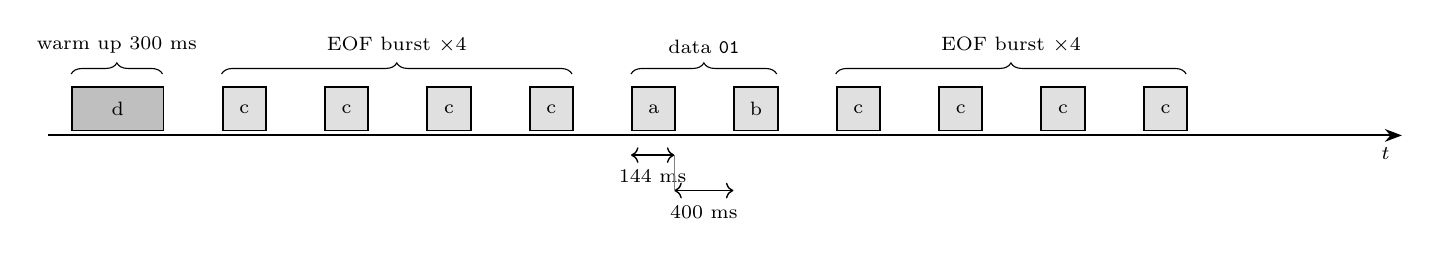
\begin{tikzpicture}[
  every node/.style={font=\scriptsize},
  tone/.style={draw, line width=0.7pt, fill=black!12, minimum height=0.55cm, anchor=south west},
  warm/.style={draw, line width=0.7pt, fill=black!25, minimum height=0.55cm, anchor=south west}
]
\draw[-{Stealth}, line width=0.7pt] (0,0) -- (17.2,0) node[below left=1pt]{$t$};
\def\toneW{0.55} \def\gapW{0.75} \def\warmW{1.16}
\node[warm, minimum width=\warmW cm] at (0.3,0.05) {d};
\def\xa{2.21}
\foreach \i/\c in {0/c,1/c,2/c,3/c}{
  \node[tone, minimum width=\toneW cm] at ({\xa+\i*(\toneW+\gapW)},0.05) {\c};
}
\def\xb{7.41}
\node[tone, minimum width=\toneW cm] at (\xb,0.05) {a};
\node[tone, minimum width=\toneW cm] at ({\xb+\toneW+\gapW},0.05) {b};
\def\xc{10.01}
\foreach \i/\c in {0/c,1/c,2/c,3/c}{
  \node[tone, minimum width=\toneW cm] at ({\xc+\i*(\toneW+\gapW)},0.05) {\c};
}
\draw[decorate, decoration={brace, amplitude=4pt}] (0.3,0.78) -- (1.46,0.78)
  node[midway, above=4pt]{warm up 300 ms};
\draw[decorate, decoration={brace, amplitude=4pt}] (\xa,0.78) -- ({\xa+3*(\toneW+\gapW)+\toneW},0.78)
  node[midway, above=4pt]{EOF burst $\times4$};
\draw[decorate, decoration={brace, amplitude=4pt}] (\xb,0.78) -- ({\xb+\toneW+\gapW+\toneW},0.78)
  node[midway, above=4pt]{data \texttt{01}};
\draw[decorate, decoration={brace, amplitude=4pt}] (\xc,0.78) -- ({\xc+3*(\toneW+\gapW)+\toneW},0.78)
  node[midway, above=4pt]{EOF burst $\times4$};
\draw[<->, line width=0.5pt] (\xb,-0.25) -- ({\xb+\toneW},-0.25);
\node[below] at ({\xb+0.5*\toneW},-0.32) {144 ms};
\draw[<->, line width=0.5pt] ({\xb+\toneW},-0.7) -- ({\xb+\toneW+\gapW},-0.7);
\node[below] at ({\xb+\toneW+0.5*\gapW},-0.77) {400 ms};
\draw[line width=0.3pt, gray] ({\xb+\toneW},-0.25) -- ({\xb+\toneW},-0.7);
\end{tikzpicture}%
}
\caption{One transmission on the air.}
\label{fig:tx-timeline}
\end{figure}

The channel is half duplex and the master enforces it at two levels: the soft core's
carrier sense is the fast reflex (hold the player, abort a tone in progress), and
the ESP32 link layer waits before every byte for 1\,s of quiet (giving up after
15\,s so a noisy decoder cannot block transmission forever). Retries exist because
the channel loses symbols routinely: a presence request unanswered for 8\,s is
repeated up to a configurable count (default 6, stored in flash), and the
registration SET is retransmitted on a randomised 30 to 40\,s timer until
acknowledged; reception is idempotent on both sides, so duplicates are harmless.

% =====================================================================
\section{Results and conclusions}
% =====================================================================

What works end to end: the bus with its ten slaves and two masters, the hand made
SDRAM controller (simulated against a behavioural die model with a self checking
GHDL testbench, then validated on the board), the 512 point FFT pipeline with its
$2.1\times$ timing margin, the snapshot path that gives the CPU clean spectra, the
NOR store after the decoupling and clock work, the display dashboard, and the acoustic
protocol between the two nodes. The design also carries its scars deliberately: the
warm up burst, the settle guard, the counter instead of the clear on read flag, the
register delay line instead of the buffer array, each one is a bench failure
turned into structure. Things tried and moved: the tone decoder, the tone emitter
and the whole flash controller all started as RTL and were re hosted in firmware
once the soft core was trustworthy, which is exactly the partition the project set
out to demonstrate, fabric for the sample rate, software for the decisions. The
most useful single lesson came from the mixed signal side: $\Delta V = I\,t/C$
explained a ``flash write succeeds but the data is not there'' bug that had looked
like firmware for days. The main residual limit is wiring, not logic: on a proper
board with a ground plane the NOR SPI would not be capped at 633\,kHz and the
retry machinery would be idle.

\end{document}


